
\newpage
\chapter[REFERENCIAL TEÓRICO]{Referencial Teórico}


Este capítulo apresenta o suporte teórico utilizado para o desenvolvimento da ferramenta. O capítulo está organizado em seções. Na primeira seção, é apresentado o Contexto Financeiro abordado, bem como a abordagem de análise financeira adotada neste Trabalho de Conclusão de Curso. Na segunda seção, é apresentada uma descrição do Paradigma de Sistemas Multiagentes explorado. Adicionalmente, é feita ainda neste capítulo uma explanação acerca das três arquiteturas comumente encontradas em Sistemas Multagentes.


\section{Contexto Financeiro}
\subsection{Mercado Financeiro}

Em um ambiente capitalista, há o interesse em aplicar recursos financeiros em troca de remuneração. Quando uma pessoa, física ou jurídica, que consome menos do que produz, tornando-se um agente superavitário, deseja investir os valores excedentes, ela procura por outra pessoa, jurídica, que tenha o interesse em captar esses valores em troca de uma remuneração. Essa remuneração é uma taxa de juros que pode ser previamente definida ou não. Assim, quando há pessoas disponibilizando valores e há em contra parte pessoas comprando esses valores, forma-se então um Mercado Financeiro (IMPORTÂNCIA do Mercado Financeiro, 2013).

Segundo a CVM, Comissão de Valores Mobiliários, o Mercado Financeiro Brasileiro é composto por quatro grandes mercados,\cite[p. 15]{cmv2014}, como ilustrado na figura 1 e brevemente apresentados nos parágrafos seguintes.

\begin{figure}[h]
\centering
\label{f01}
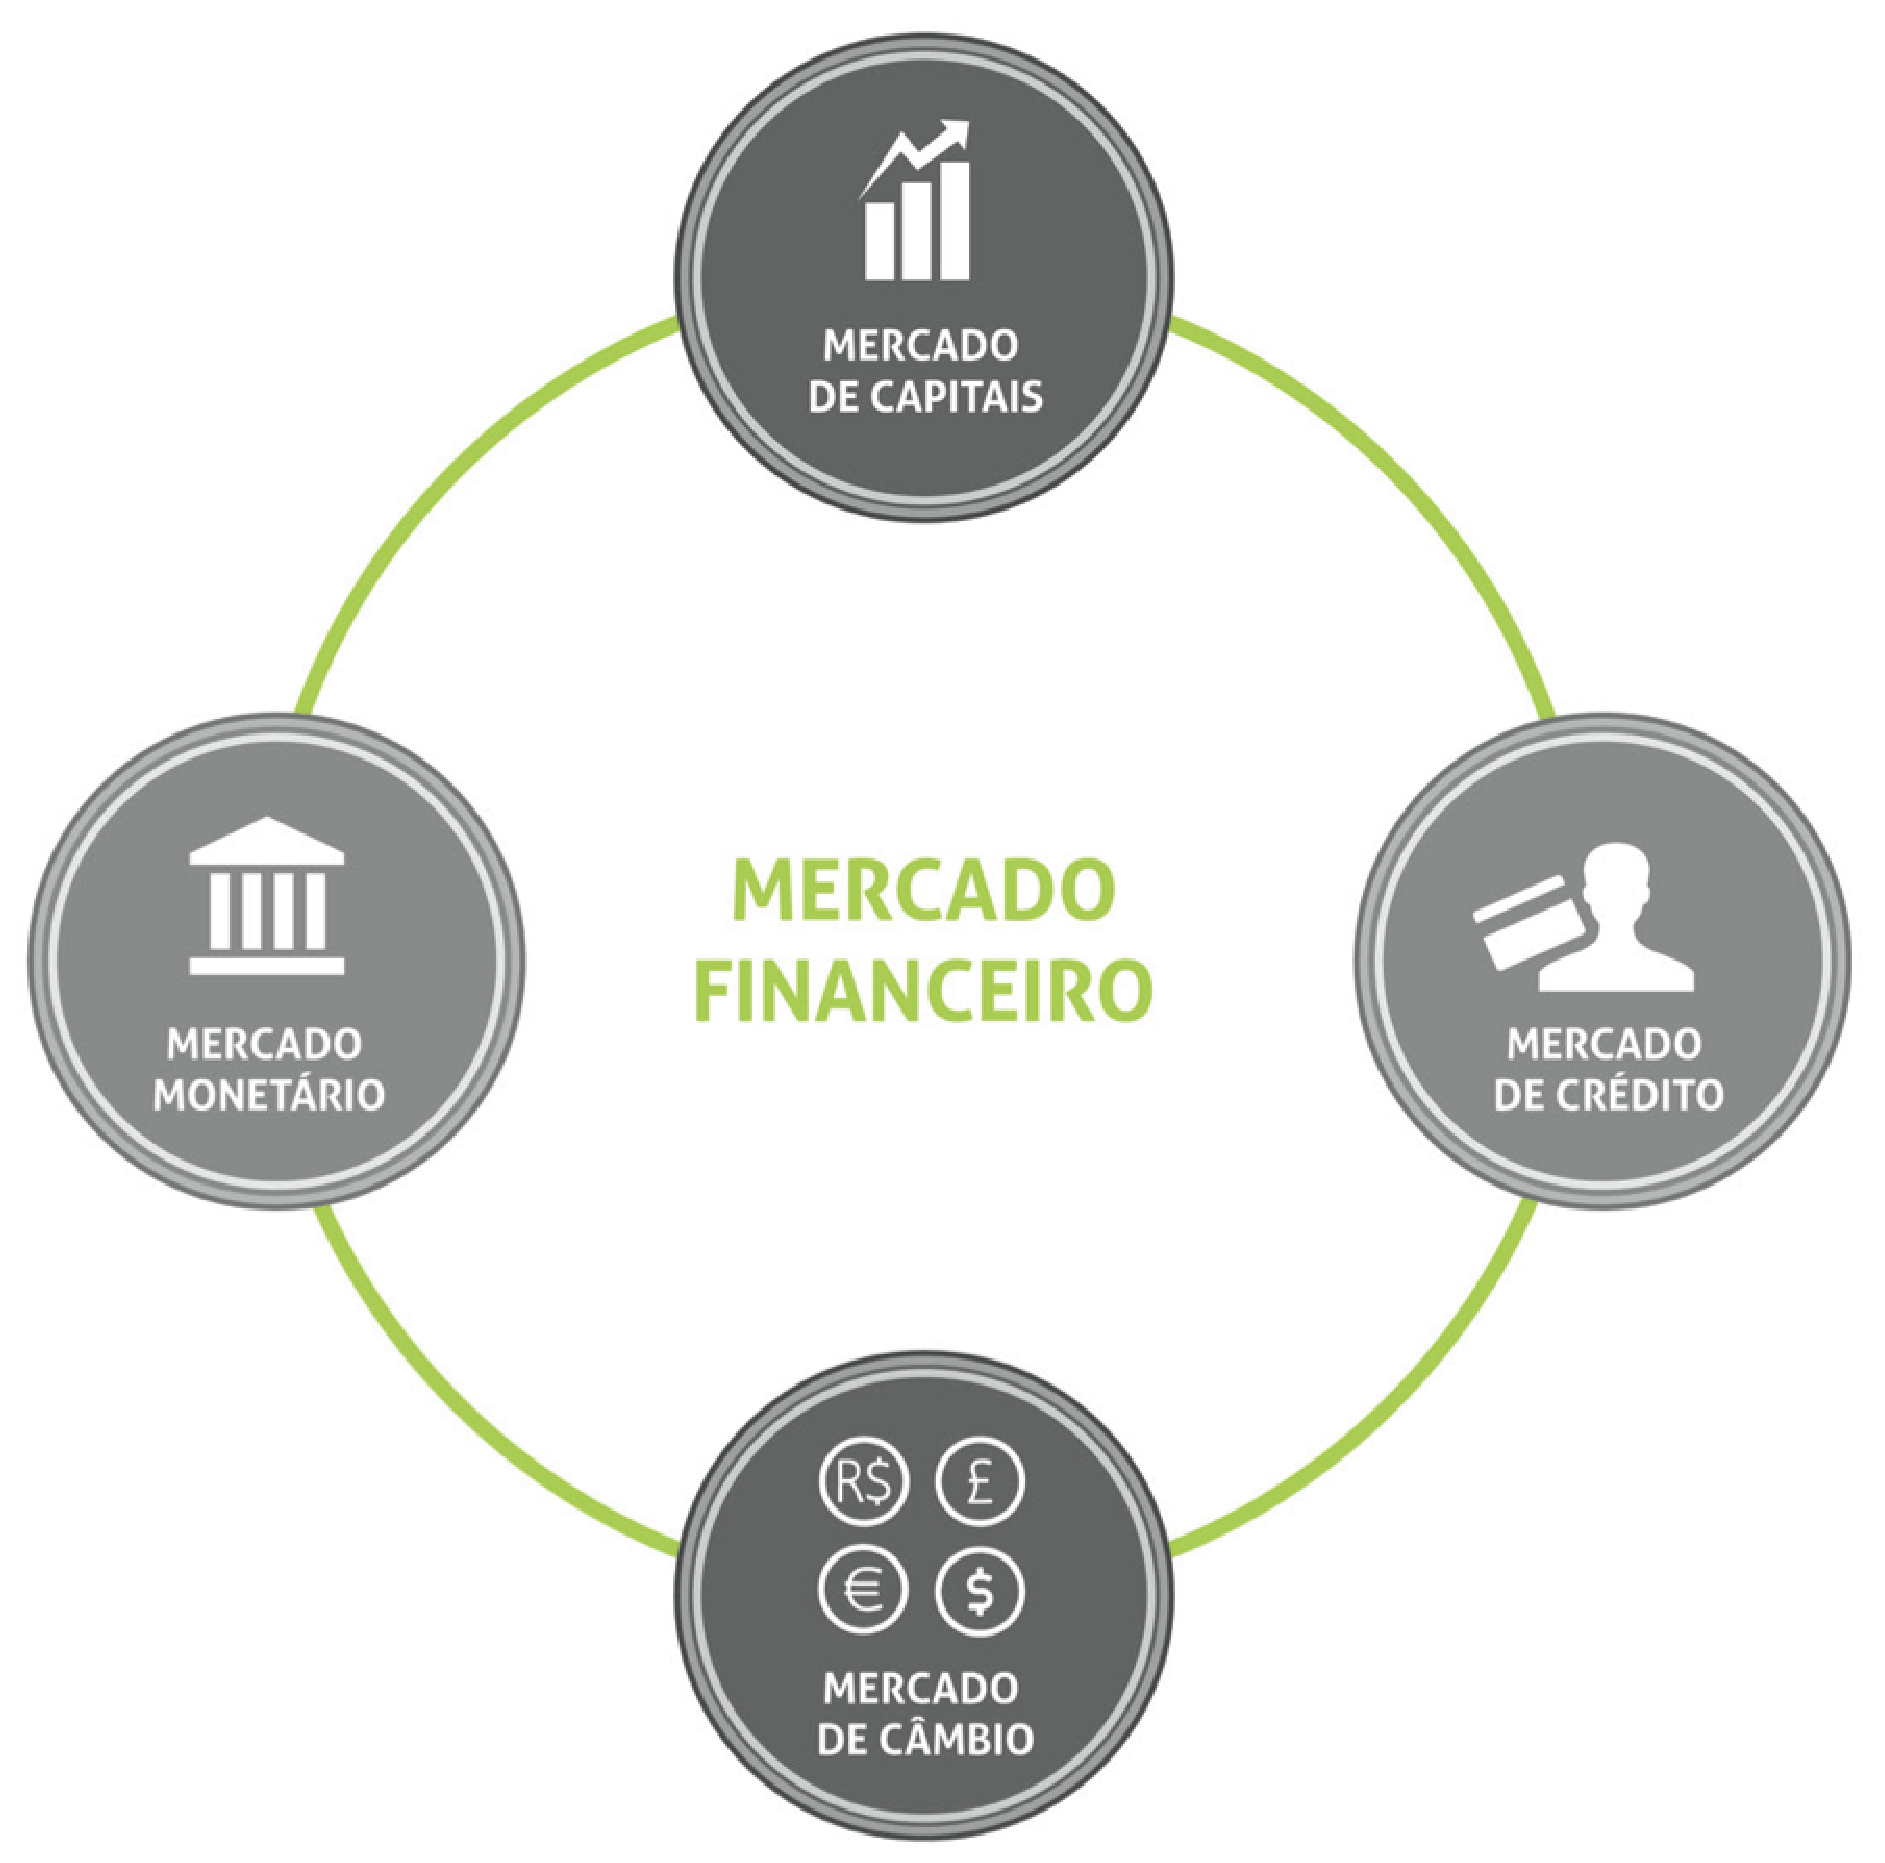
\includegraphics[width=0.5\textwidth]{figuras/f01}
\caption{Composição Mercado Financeiro Brasileiro  \newline fonte: CVM,2013}

\end{figure}

O Mercado Monetário é um mercado onde os participantes são instituições financeiras, nas quais há diversas transferências de valores em curto prazo, cerca de um dia. Essas transferências são realizadas entre elas e/ou entre elas e o Banco Central, Bacen. O Banco Central, por sua vez, realiza intervenções neste mercado, visando realizar controles em concordância com a Política Monetária Nacional. Política essa que influencia diretamente no controle inflacionário da economia \cite[p. 32]{cmv2014}.

O Mercado de Crédito é o mercado onde instituições financeiras captam dinheiro de agentes superavitários e realizam empréstimos a pessoas físicas ou jurídicas. Esta instituição tem um compromisso com o agente superavitário comprovado por títulos privados. Ao emprestar um valor à uma pessoa, esta instituição financeira é remunerada com a diferença de juros que cobra do devedor e paga ao seu credor (agente superavitário), denominado \textit{spread}, pelos serviços de intermediação. O Bacen é o principal órgão regulador deste mercado para evitar que ocorram casos de lucros abusivos \cite[p. 32]{cmv2014}.

O Mercado de Câmbio é um mercado onde há transações entre moedas estrangeiras e a moeda nacional. Participam deste mercado instituições que possuem despesas ou receitas em moeda estrangeira. O Bacen é o órgão que regula este mercado visando mantê-lo em concordância com a Política Cambial\cite[p. 32]{cmv2014}.

O Mercado de Capitais é o mercado onde empresas captam valores diretamente com os agentes superavitários, através de títulos como Debêntures, notas promissórias, ações, dentre outros. Em outras palavras, o risco da operação é assumido pelo agente superavitário e não mais pela instituição que faz a intermediação, como no Mercado de Crédito. Porém, essa captação é assessorada por uma empresa apropriada que presta estes serviços. Este mercado é regulado pela CVM (\citeyear{cmv2014},p 33).Os participantes deste mercado estão apresentados no tópico subsequente, uma vez que este será o mercado abordando neste TCC.

\subsection{Mercado Capitais}

Suponha que uma empresa, cujo nome fantasia seria XPTO S.A, tenha interesse em fazer alguns investimentos em seus projetos. Essa empresa poderá financiar seus investimentos de três maneiras: (i) usando recursos próprios através do lucro acumulado ao longo do tempo; (ii) com base em financiamentos de instituições especializadas em venda de crédito; (iii) ou mesmo através do mercado de capitais, com emissão pública de títulos.
	
Ao optar pela terceira alternativa, a empresa deverá iniciar, junto com a CVM, um processo de abertura de capital. Depois, deverá atender os critérios estipulados por essa comissão reguladora. Por fim, poderá disponibilizar publicamente suas ações  em um Mercado de Capitais. 

Ao conseguir a abertura de capital autorizada pela CVM, a empresa emite ações que são adquiridas pelos agentes superavitários, os quais podem ser chamados de investidores, por intermédio de corretoras de valores devidamente registradas. Essas últimas, por sua vez, enviam esses valores à Bolsa de Valores, na qual se encontra a ação disponível. No Brasil, a Empresa responsável por promover um ambiente transparente e líquido para realização dessas negociações é a BM\&FBovespa, sediada na capital do Estado de São Paulo.

Para realizar negociações de valores mobiliários, um investidor pode ou não seguir alguma estratégia, que por sua vez pode ou não ser baseada em estudos de especialistas. Estes estudos dividem a atividade de análise de mercado em duas abordagens: a Análise Técnica \cite{noronha2010} e a Análise Fundamentalista \cite{buffet2010}, de um ativo, ambas aplicadas ao Mercado de Ações .

Na abordagem da Análise Técnica, são considerados apenas dados como preço e volume da ação. Em posse destas informações, o analista elabora gráficos, realiza diversos cálculos, usa indicadores matemáticos no intuito de detectar padrões comportamentais do mercado. Vale observar que nesta abordagem não importa de qual empresa pertence a ação, pois o analista deseja encontrar somente os padrões comportamentais dos investidores, para assim elaborar estratégias que retornem o maior lucro possível.

Na abordagem da Análise Fundamentalista, são considerados dados como: (i) Lucro bruto/Margem de lucro bruto; (ii) despesas operacionais; (iii) despesas; (iv) balanço patrimonial  entre outros \cite{buffet2010}. O analista realiza cálculos para encontrar o preço justo da ação desta empresa e o confronta com o valor corrente no mercado, assim realiza operações de compra e/ou venda quando suas estratégias indicam o melhor momento para operar. Diferente do analista técnico, é importante para o analista fundamentalista conhecer a empresa investida.

São adotadas, neste TCC, técnicas financeiras pertencentes à abordagem da Análise Técnica. Técnicas estas desenvolvidas por especialistas no mercado de capitais e publicadas em mídia impressa e/ou virtual.


\section{Engenharia de Software}
\subsection{Sistemas Multagentes}
\subsubsection{Agentes}

Russel e Norving (\citeyear{russel2003}, p. 31) definem: \textit{“An agent is anything that can be viewed as perceiving its environment through sensors and acting upon that environment through actuators”}. Em outras palavras, um agente é capaz de se comportar em um determinado ambiente de acordo com as informações oriundas deste ambiente, seja ele determinístico ou não.

Segundo Wooldridge, um agente possui as seguintes características: (i) Autonomia, não há intervenções no processo de decisão de um agente. Ele toma decisões sem intervenções de outros agentes ou humanos; (ii) Sociabilidade, um agente interage com outros agentes, Software ou humano, através de algum tipo de linguagem de comunicação de agentes, e têm a habilidade de trabalhar em conjunto com outros agentes afim de alcançar um objetivo; (iii) Reatividade, um agente fica situado em um ambiente e é capaz de perceber esse ambiente através de seus sensores, sendo capaz ainda de responder em tempo hábil às mudanças que ocorrem nele; e (iv) Pró-atividade, um agente não apenas responde às mudanças do ambiente, ele é capaz de tomar iniciativa \cite[p. 2-3]{wooldrige2002}.

De acordo com Girardi (\citeyear{girardi2004}, p. 5), o mecanismo utilizado para a tomada de decisão da ação a ser executada a partir de uma percepção é o que distingue um agente, classificando-o em um agente: (i) deliberativo, quando a tomada de decisão da ação a ser executada é realizada via raciocínio lógico em concordância com um plano de ações para atingir alguma meta; (ii) reativo, quando o agente não possui um modelo do ambiente, agindo apenas em reposta a estímulos do ambiente no qual está inserido, sendo assim, um agente reativo não conhece o ambiente ao qual pertence; e (iii) híbrido, quando um agente possui características de um agente deliberativo e de um agente reativo \cite[p. 5]{girardi2004}. 

\subsubsubsection{Agentes Comportamentais}

Um agente comportamental é um agente reativo, que tem seus comportamentos abstraídos de comportamentos de uma entidade do mundo real, normalmente \cite[p. 33]{oliveira2008}. Um conjunto de agentes comportamentais, de maneira cooperativa, pode ser utilizado para solucionar um problema complexo. Um exemplo comumente encontrado na literatura, é o da colônia de formigas. Neste cenário, cada formiga é uma entidade simples, mas em conjunto é capaz de realizar trabalhos complexos existentes em uma colônia, por exemplo: construir um formigueiro semelhante ao da figura 2.

\begin{figure}[h]
\centering
\label{f02}
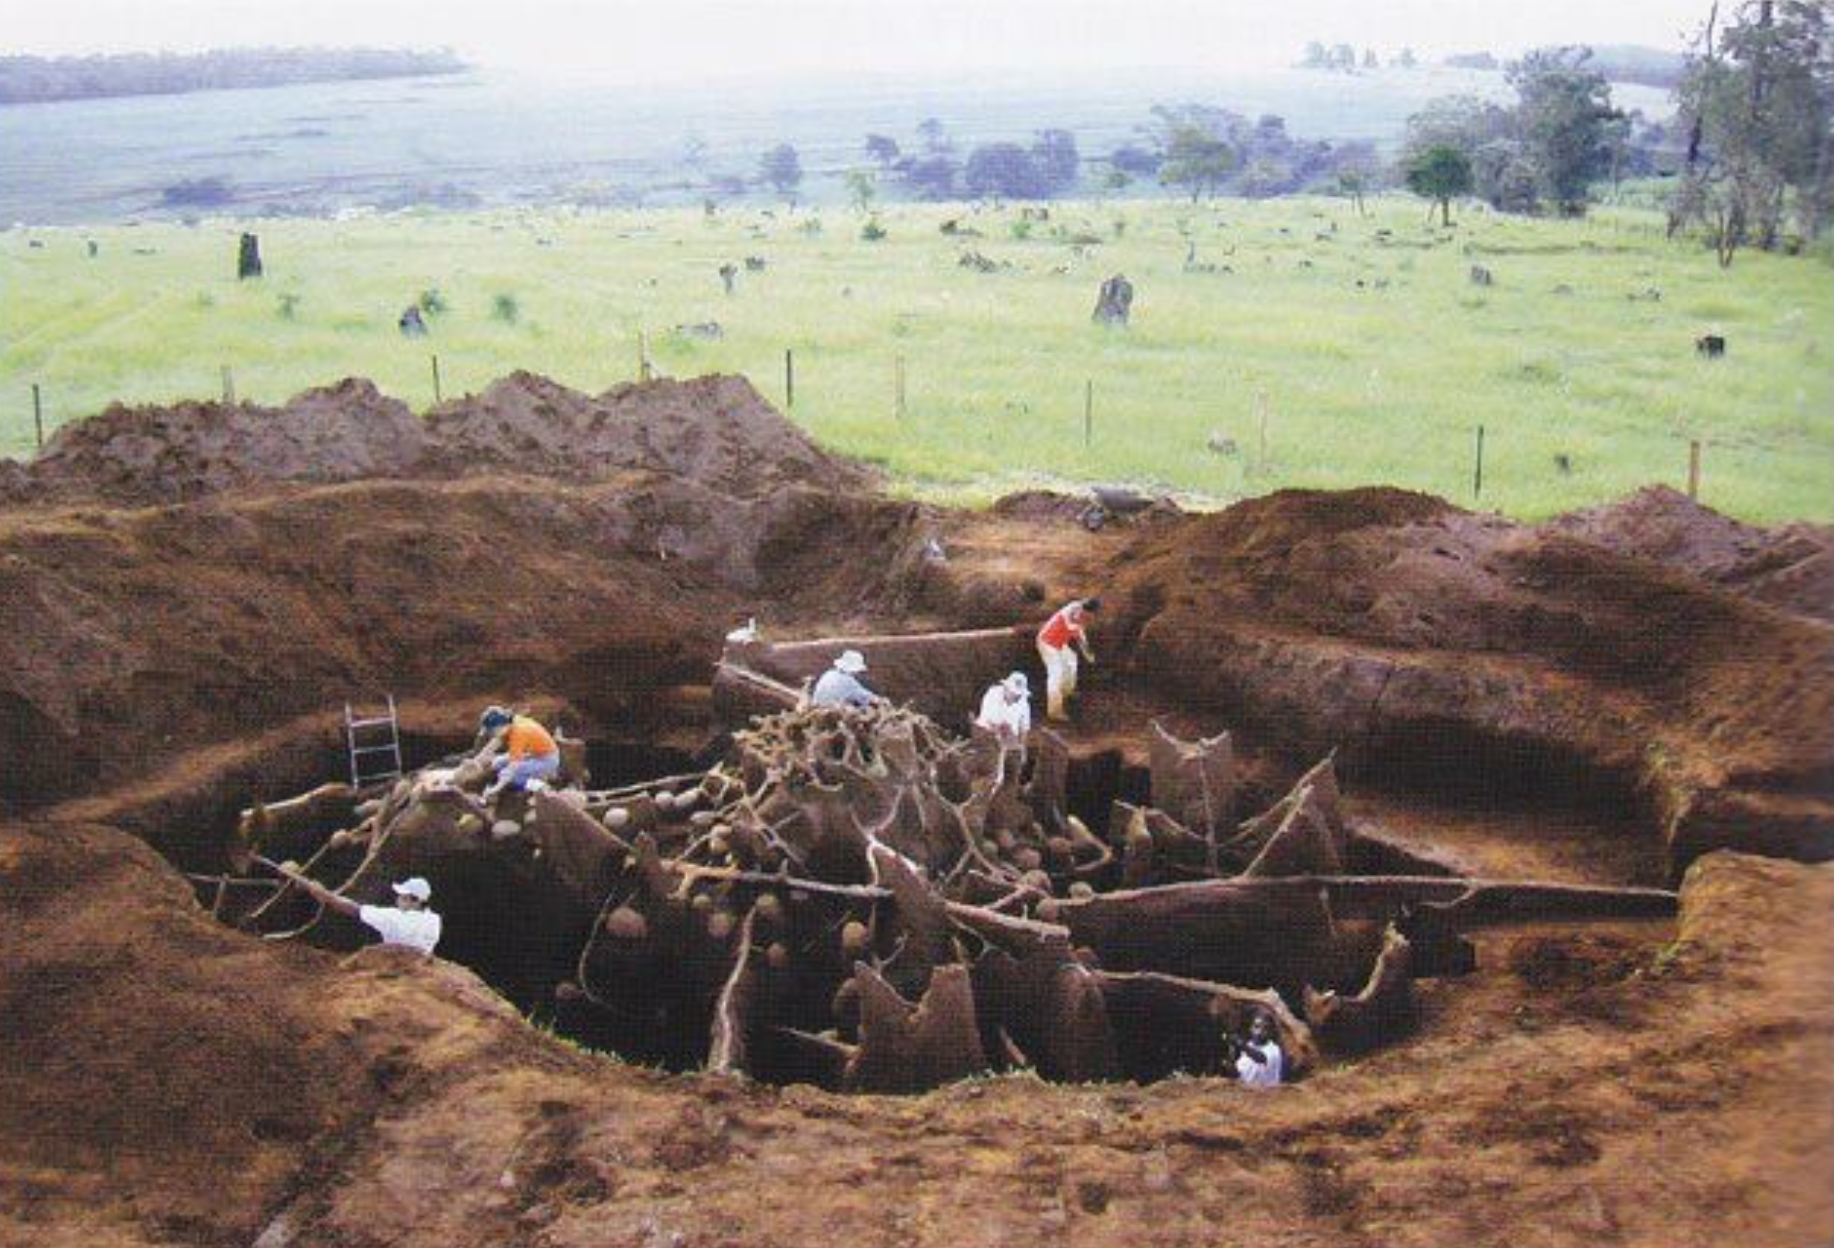
\includegraphics[width=0.5\textwidth]{figuras/f02}
\caption{Formigueiro\newline Fonte: National Geographic}

\end{figure}

As formigas são dividas por tipos de trabalhos, assim temos as seguintes entidades, ou agentes comportamentais: (i) Rainhas, formigas responsáveis por pôr ovos que darão origem a novas formigas da colônia; (ii) Operárias, formigas que realizam tarefas de acordo com a sua idade e tamanho, e (iii) Machos, formigas que vivem apenas o suficiente para fecundar a Rainha. Em uma colônia, as formigas Operárias mais novas e menores ficam responsáveis por atividades de alimentar a Rainha e lavas, e de limpeza do formigueiro. Já para as operárias mais velhas, ficam as atividades de maior risco, como a proteção do formigueiro (para formigas maiores) e a busca por novas fontes externas de alimento \apud[p. 35]{holldobler1990} {oliveira2008}.

Alvares e Sichman (\citeyear{alvares1997}, p. 12) destacam do exemplo das formigas características dos sistemas multiagentes reativos:

\begin{citacao}
\begin{enumerate}

	\item Não há representação explícita de conhecimento- o conhecimento dos agentes é implícito e se manifesta através do seu comportamento;

	\item Não há representação do ambiente- o seu comportamento se baseia no que é percebido a cada instante do ambiente, mas sem uma representação explicita deste; 

	\item Não há memória das ações – o agentes reativos não mantém um histórico de suas ações, de forma que o resultado de uma ação passada não exerce nenhuma influência sobre as suas ações futuras;


	\item Organização etológica – a forma de organização dos agentes reativos é similar a dos animais, em oposição à organização social dos sistemas cognitivos;

 	\item Grande número de membros – os sistemas multiagentes reativos têm, em geral, um grande número de agentes, da ordem de dezenas, centenas ou mesmo milhões de agentes.
 	\newline \cite[p. 12]{alvares1997}.

\end{enumerate}
\end{citacao}


\subsubsubsection{Agentes Intencionais}

Quando um aluno deixa a universidade com uma primeira graduação, ele se depara com uma decisão a tomar, sobre o que fazer com sua vida. O processo de decisão tipicamente inicia-se tentando entender as opções disponíveis em função do conhecimento (crenças) que o aluno possui do seu ambiente. Por exemplo, se o aluno tem um bom histórico escolar, então uma opção é se tornar um acadêmico. Outra opção é se tornar um profissional. Após a geração do grupo de alternativas (desejos), deve-se optar por uma e se comprometer com ela. Esta escolha vem a ser sua intenção. As intenções alimentam o raciocínio lógico futuro do agente. Por exemplo, se o aluno decidir que quer se tornar um acadêmico, então ele deve comprometer-se com esse objetivo e despender tempo e esforço para alcançá-lo. \apud[p. 4] {wooldridge1999}{girardi2004}.

Agentes deliberativos são agentes capazes de decidir de maneira autônoma seus objetivos e os mudar no decorrer do tempo. Ou seja, estes agentes apresentam uma considerável capacidade cognitiva. Agentes deliberativos possuem as seguintes características:
\begin{citacao}
\begin{enumerate}

	\item Mantêm uma representação explicita de seu ambiente e dos outros agentes;
	\item Podem manter um histórico das interações e ações passadas, isto é, têm memória do passado;
	\item A comunicação entre os agentes é feita de modo direto, através do envio e recebimento de mensagens;
	\item Seu mecanismo de controle é deliberativo, ou seja, tais agentes raciocinam sobre quais objetivos devem alcançar, quais planos seguir e quais ações devem ser executadas num determinado momento;
	\item Seu modelo de organização é baseado em modelos sociológicos, como organizações humanas;
	\item Uma sociedade contém tipicamente poucos agentes, na ordem de uma dezena.
	 \newline \apud[p. 28]{ferber1991}{alvares1997}

\end{enumerate}
\end{citacao}

Um modelo de agente deliberativo bastante investigado na Inteligência Artificial é o modelo Belief-Desire-Intention (BDI) \apud[p. 30]{bratman1999}{serrano2011}. Neste modelo, o raciocínio humano é representado através de crenças, desejos e intenções. As crenças formam o conhecimento do agente, e estas são abstrações de informações do mundo real. Os desejos são as metas do agente; são a razão por trás das ações dos agentes. As intenções são as ações do agente; são as sequências de tarefas que o agente desempenha para atender um desejo que está associado às suas crenças \cite[p. 31]{serrano2011}.

\subsubsection{Sistemas Multiagentes (SMA)}

Girardi (\citeyear{girardi2004}, p.6) caracteriza um sistema multiagentes (SMA) como \textit{“um grupo de agentes que atuam em conjunto no sentido de resolver problemas que estão além das suas habilidades individuais. Os agentes realizam interações entre eles de modo cooperativo para atingir uma meta.”} Girardi (\citeyear{girardi2004}, p.7) define ainda, \textit{“A arquitetura  de um SMA mostra a maneira como o sistema está implementado em termos de propriedades e estrutura e como os agentes que o compõe podem interagir a fim de garantir a funcionalidade do sistema.”}

 Esta arquitetura pode ser classificada dentre três grupos, conforme sua complexidade: (i) Arquitetura simples: composta apenas por um agente. (ii) Arquitetura moderada, composta por agentes que executam as mesmas tarefas, mas possuem diferentes usuários, sendo que estes agentes podem ainda ser distribuídos em diversos computadores e cooperar entre si. (iii) Arquitetura complexa, composta por agentes de diversos tipos, estes também podem ser distribuídos em diversos computadores e cooperar entre si. As arquiteturas podem ser classificadas considerando seu mecanismo de cooperação e coordenação \apud[p. 7]{knapik1998}{girardi2004}.

Através de um mecanismo de cooperação, os agentes de um SMA expõem suas necessidades para outros agentes. Segundo Girardi, este mecanismo de cooperação é abordado de maneira destacada em três padrões arquiteturais para o desenvolvimento de um SMA: a (i) arquitetura quadro-negro; a (ii) arquitetura de troca de mensagens; e a (iii) arquitetura federativa.\cite[p. 7]{girardi2004}. 

Na arquitetura quadro-negro, os agentes se comunicam com outros agentes através de um repositório (organizado em regiões ou níveis para facilitar a busca de informações), que concentra todas as mensagens emitidas por eles, uma espécie de memória compartilhada utilizada por um SMA. Os agentes vão atendendo às mensagens à medida em que vão acessando o quadro-negro \cite[p. 7]{girardi2004}.

Na arquitetura de troca de mensagens, os agentes comunicam-se diretamente uns com os outros através de mensagens assíncronas. Assim, torna-se necessário que cada agente saiba os nomes e endereços dos outros agentes que compõem o SMA. Para que as mensagens ocorram de maneira adequada entre os agentes, é necessário um protocolo de comunicação entre agentes. É no protocolo que estão as regras, as quais agregam um formalismo adequado, e serão seguidas pelos agentes para se obter a melhor comunicação possível \cite[p. 8]{girardi2004}.

Na arquitetura federativa, os agentes são organizados em grupos ou federações. Em cada grupo/federação existe um agente facilitador responsável por receber as mensagens que chega para cada grupo/federação e encaminhá-las para os agentes destinatários presentes no grupo. Ou seja, nesta arquitetura os agentes se comunicam somente através de um agente facilitador \cite[p. 8]{girardi2004}.


\subsubsection{Agentes e Objetos}

O paradigma de agentes surge como uma evolução natural da orientação a objetos. Como os objetos, a abstração agente possui uma memória e um comportamento. Porém, ela não é uma entidade passiva como os objetos tradicionais. A priori, um agente pode ser definido como um objeto ativo, autônomo, social e com capacidade de aprendizado. 
\newline \apud[p. 2]{girardi2001,hyacinth1996,wooldridge1999} {girardi2004}.


De acordo com Wooldridge, Objetos são definidos como entidades computacionais que encapsulam algum estado, são capazes de realizar ações, ou métodos neste estado, e se comunicar por passagem de mensagens. Wooldridge aponta, ainda, três significantes diferenças entre Objetos e Agentes \cite[p. 25-27]{wooldrige2002}. 

A primeira é o grau de autonomia de Objetos e Agentes, um objeto tem controle sobre seu estado interno, mas não tem controle sobre seu comportamento. Caso um método seja disponibilizado para outros objetos invocarem, eles podem fazer isso a qualquer momento que desejarem. Assim, um objeto não tem controle se o método é executado ou não. Entretanto, um agente ao receber uma requisição, tem o poder de decidir se irá atender ou não. A segunda é a respeito da noção de comportamento autônomo flexível (i.e. reatividade, pró-atividade e habilidade social). A terceira é que cada agente tem sua própria \textit{thread} de controle,\cite[p. 25-27]{wooldrige2002}.


\section{Resumo do Capítulo}

Esse capítulo elucidou o Contexto Financeiro, apresentando como o Mercado Financeiro Brasileiro é composto por quatro tipos de mercado \cite[p. 15]{cmv2014}: (i) Mercado Monetário, que é um mercado exclusivo para instituições financeiras; (ii) Mercado de Crédito, mercado onde atuam empresas financeiras especializadas em empréstimos como bancos públicos e privados; (iii) Mercado de Câmbio, onde atuam empresas que normalmente têm despesas e/ou receitas em moeda estrangeira; e (iv) Mercado de Capitais, que é o mercado abordado neste estudo de TCC. Em Engenharia de Software, foi apresentada uma definição de agentes de Software, reforçando suas características quando os mesmos são reativos ou deliberativos. Adicionalmente, ainda sobre Sistemas Multiagentes, comentou-se sobre três arquiteturas comumente encontradas em SMA, tais como: a (i) arquitetura de quadro negro; a (ii) arquitetura de troca de mensagens; e a (iii) arquitetura federativa.
\newpage
\FloatBarrier
\chapter[SUPORTE TECNOLÓGICO]{Suporte Tecnológico}

Este capítulo apresenta o suporte tecnológico utilizado para o desenvolvimento da ferramenta. O capítulo está organizado em seções. Na primeira seção, são apresentadas ferramentas comumente utilizadas em análises técnicas da Bolsa de Valores. Na segunda seção, são apresentados os padrões de projetos adotados no desenvolvimento da ferramenta, bem como o padrão arquitetural adotado com propósito de contribuir com a manutenabilidade e extensibilidade da ferramenta. Adicionalmente, ainda nessa seção, é apresentada uma descrição mais detalhada do framework JADE. Por fim, é apresentada a metodologia Ágil que foi adaptada para conduzir o desenvolvimento da ferramenta acordada por este Trabalho de Conclusão de Curso.


\section{Contexto Financeiro}

Novos recursos tecnológicos são criados periodicamente, sejam linguagens de programação, novas formas de se solucionar um problema, novos produtos derivados da eletrônica, entre outros. No contexto financeiro não é diferente, ferramentas voltadas ao mercado de capitais, com intuito de automatizar as operações de um investidor neste mercado, encontram-se à disposição.

No entanto, as ferramentas disponíveis ao investidor são ferramentas que o auxiliam na atividade de análise de investimentos, tais como ferramentas de análise técnica. Já outras são serviços oferecidos por \textit{sites} de empresas especializadas, as quais sugerem ao investidor quais papéis são bons de serem comprados ou vendidos. Há ainda ferramentas que apenas auxiliam no acompanhamento da evolução dos investimentos. Percebe-se, então, uma característica em comum entre estas ferramentas, ou seja, é preciso que o investidor tenha bons conhecimentos relacionados ao mercado para que o mesmo possa desfrutar ao máximo dos recursos que essas ferramentas oferecem. Diante disto, a ferramenta desenvolvida nesse TCC abstrai tais conhecimentos e delega ao usuário apenas a decisão em comprar ou vender uma ação. Algumas ferramentas avaliadas neste Trabalho de Conclusão de Curso encontram-se elencadas a seguir.

\subsection{Ferramentas de análise técnica}

\subsubsection{GrapherOC}

O GrapherOC (figura 3) é um Software de apoio ao acompanhamento do mercado. Com essa ferramenta, o investidor pode testar suas estratégias, obter cotações em tempo real e enviar ordens para corretora. Este Software permite ao investidor criar estratégias e programá-las. No entanto, tal suporte exige que o investidor já possua conhecimentos em estratégias financeiras. Trata-se, por fim, de uma ferramenta disponível somente para computadores com o sistema operacional Windows 7 \textregistered   ou superior instalado, não sendo compatível, portanto, com outros sistemas operacionais.


\begin{figure}[h]
\centering
\label{f03}
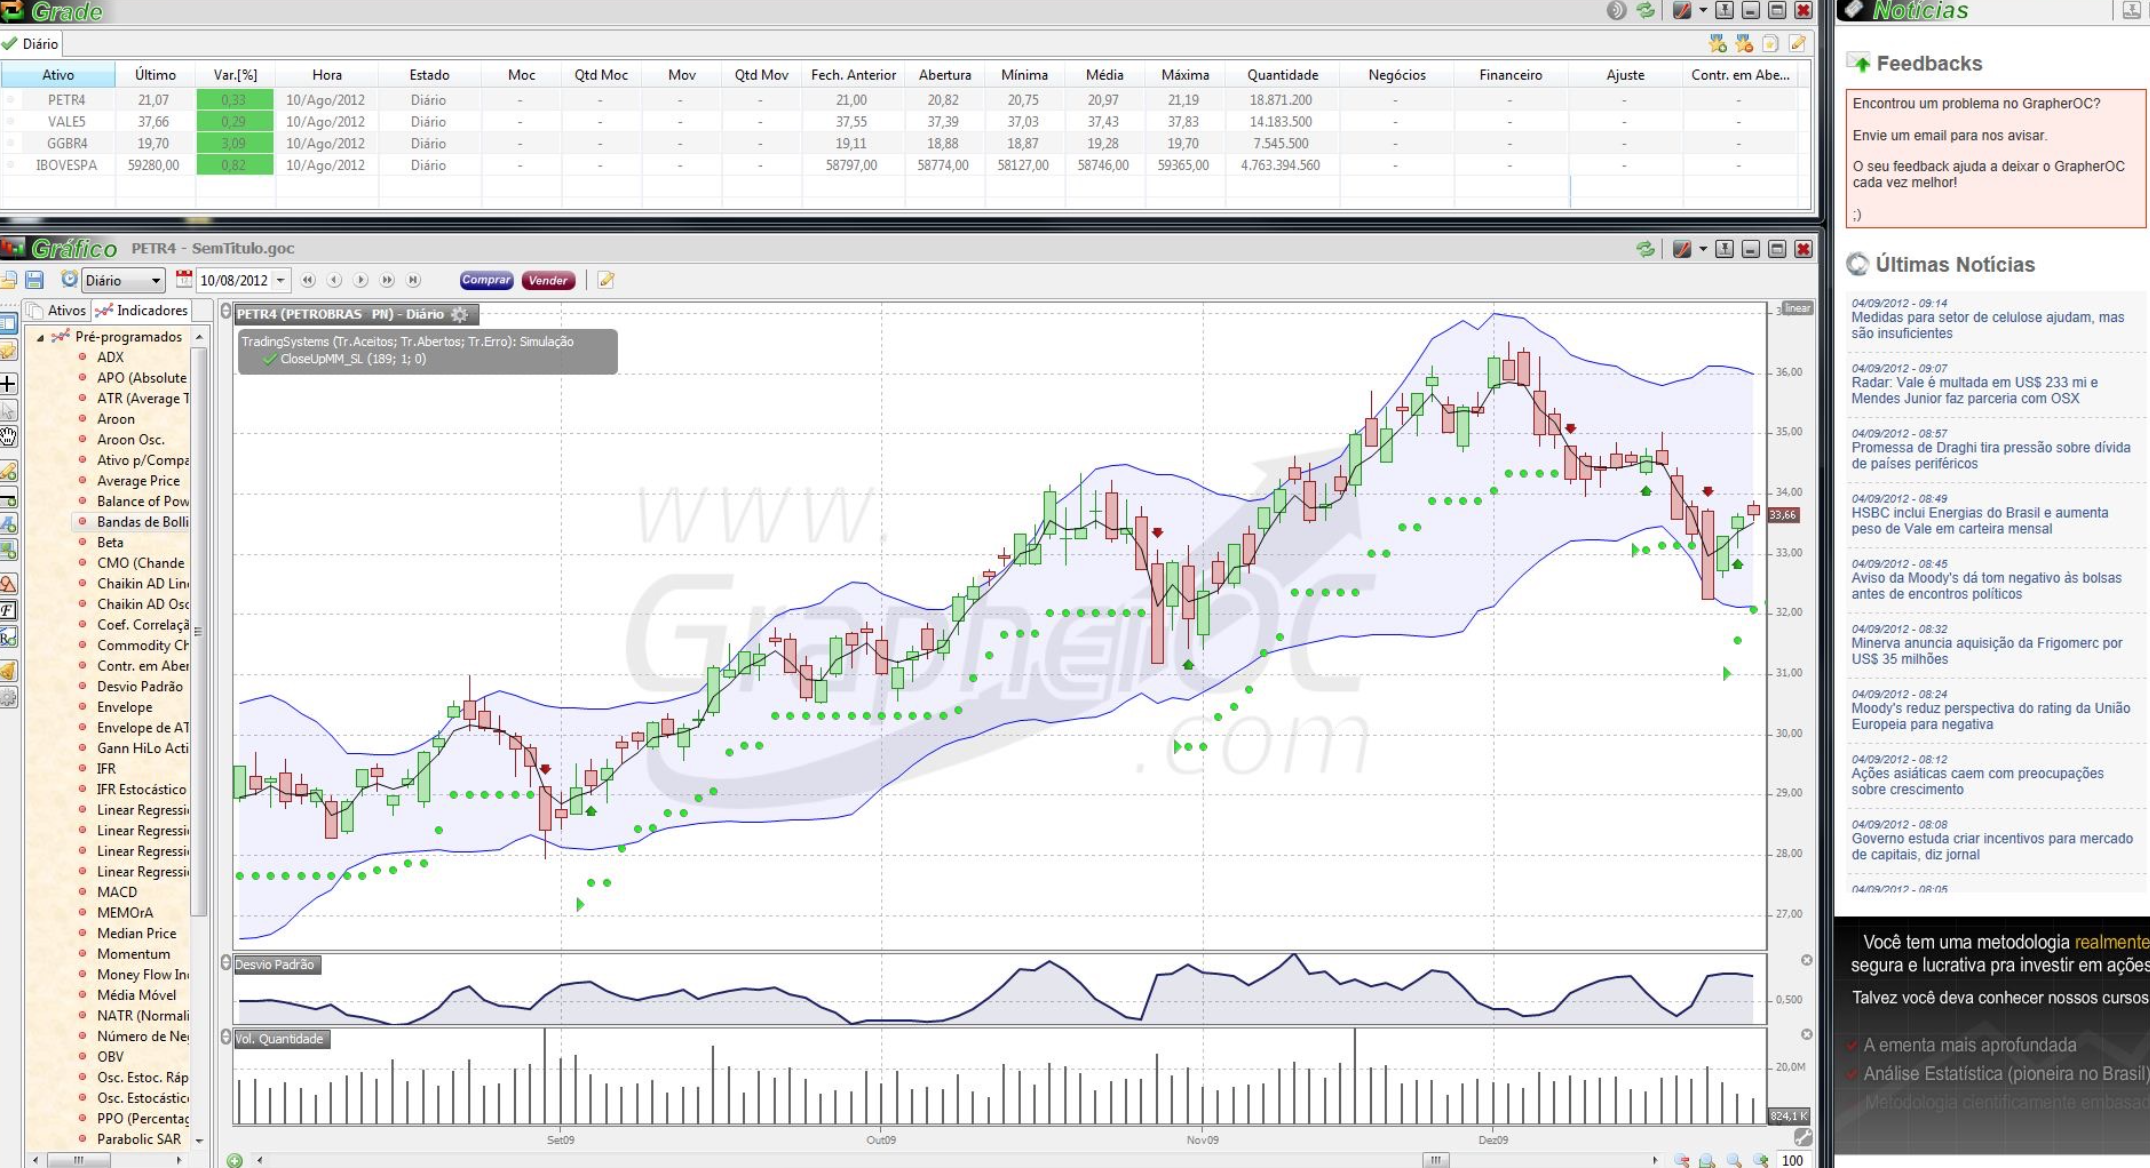
\includegraphics[width=0.8\textwidth]{figuras/f03}
\caption{GrapherOC}

\end{figure}

\subsubsection{Ferramentas de corretoras}

Corretoras de valores, como a XP Investimentos e Ágora (figura 3), disponibilizam ao seus clientes ferramentas de envio de ordens de compra e venda (HomeBroker), bem como ferramentas de suporte para atividades de análise técnica. Porém, para usufruir o máximo possível delas, é requerido do usuário conhecimentos financeiros relacionados à análise técnica. No entanto, caso o cliente não tenha tais conhecimentos, as corretoras, normalmente, oferecem acompanhamento de profissionais capacitados para atuar no mercado.

\subsubsection{Meta Trader}

O MetaTrader (figura 4) é uma plataforma oferecida por corretoras estrangeiras. Essa ferramenta aborda o mercado de moedas (FOREX) e o de \textit{commodities}, tais como petróleo. A plataforma possui um suporte tecnológico oferecido ao usuário, conferindo ao mesmo uma IDE para desenvolver produtos de Software, conhecidos por robôs, em uma linguagem própria, Mql4 \cite{kovalyov2006}. A linguagem Mql4 é uma linguagem estruturada, baseada na linguagem C, e sua evolução é o Mql5 \cite{metaquotes2014}, a qual é uma linguagem orientada a objetos. No entanto, essa ferramenta requer do usuário conhecimentos relacionados ao Mercado Financeiro, além de conhecimentos de lógica de programação.

\begin{figure}[h]
\centering
\label{f04}
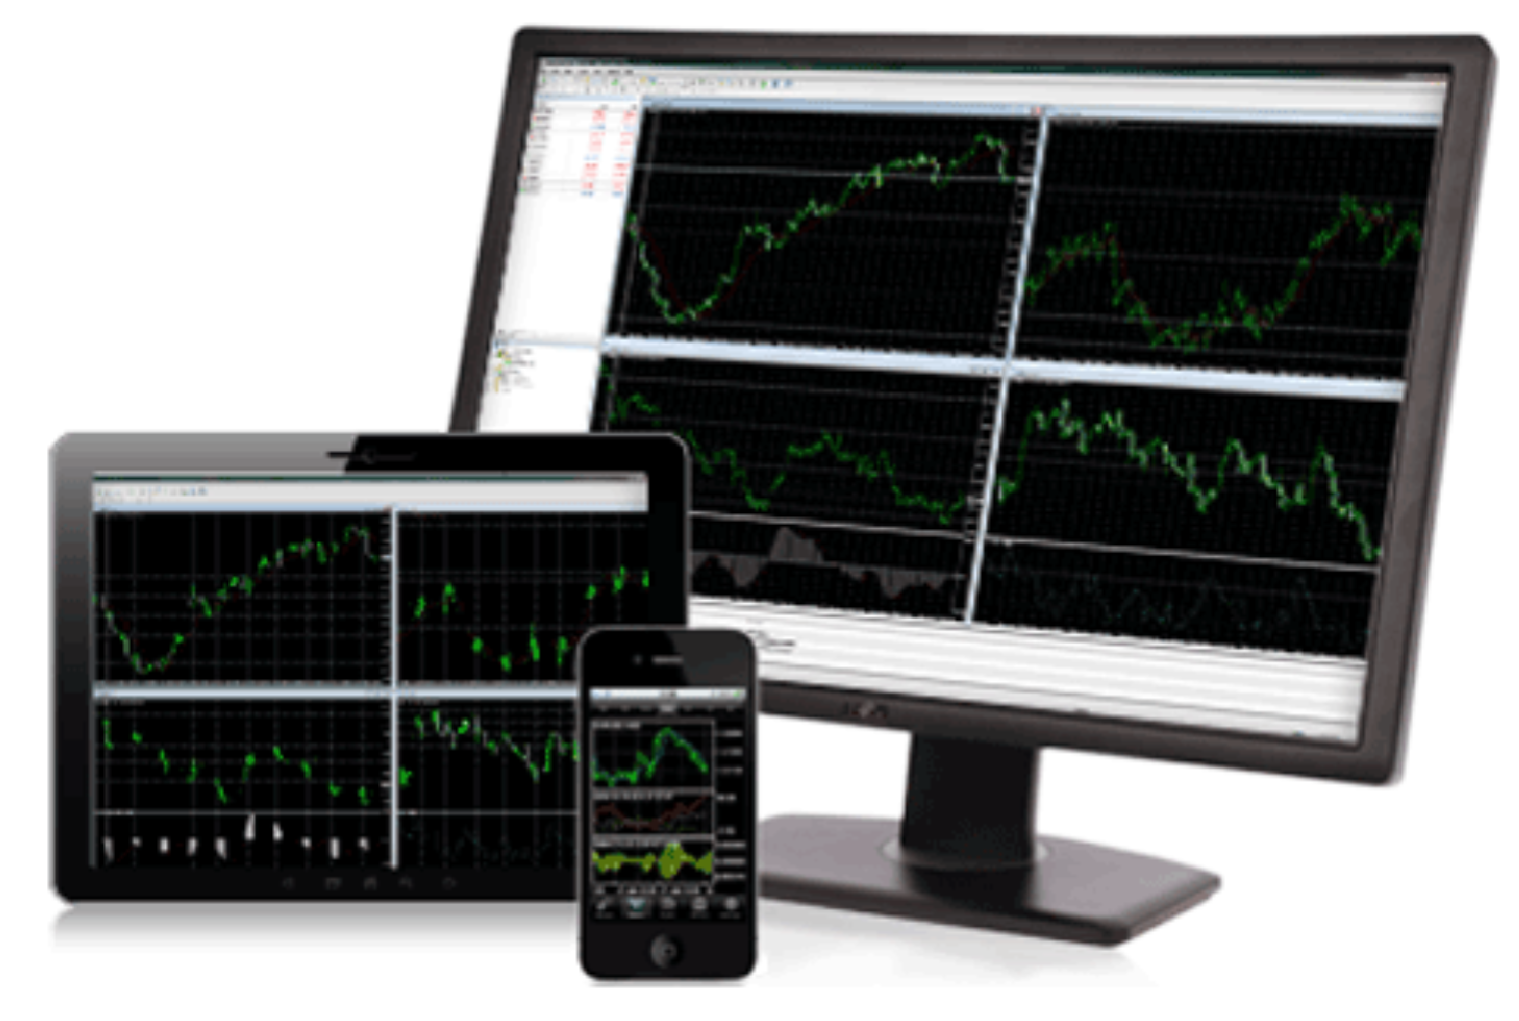
\includegraphics[width=0.5\textwidth]{figuras/f04}
\caption{MetaTrader}

\end{figure}


\subsubsection{Grafix}

O Grafix (figura 5) é uma ferramenta somente para análise gráfica. Tornou-se Software livre no ano de 2012. Trata-se de um suporte construído em Java e seu desenvolvimento está estagnado, desde 2012, por falta de voluntários no desenvolvimento. Assim como as demais, essa ferramenta também exige de seus usuários conhecimentos relacionados a investimentos bem como se diferencia por não ser possível ao investidor enviar ordens de compra/venda diretamente por ela. Limita-se, portanto, apenas em possibilitar a análise do mercado de ações. No entanto, por ser um Software livre, esse suporte permite modificações, sendo possível incorporar novas funcionalidades.

\begin{figure}[h]
\centering
\label{f05}
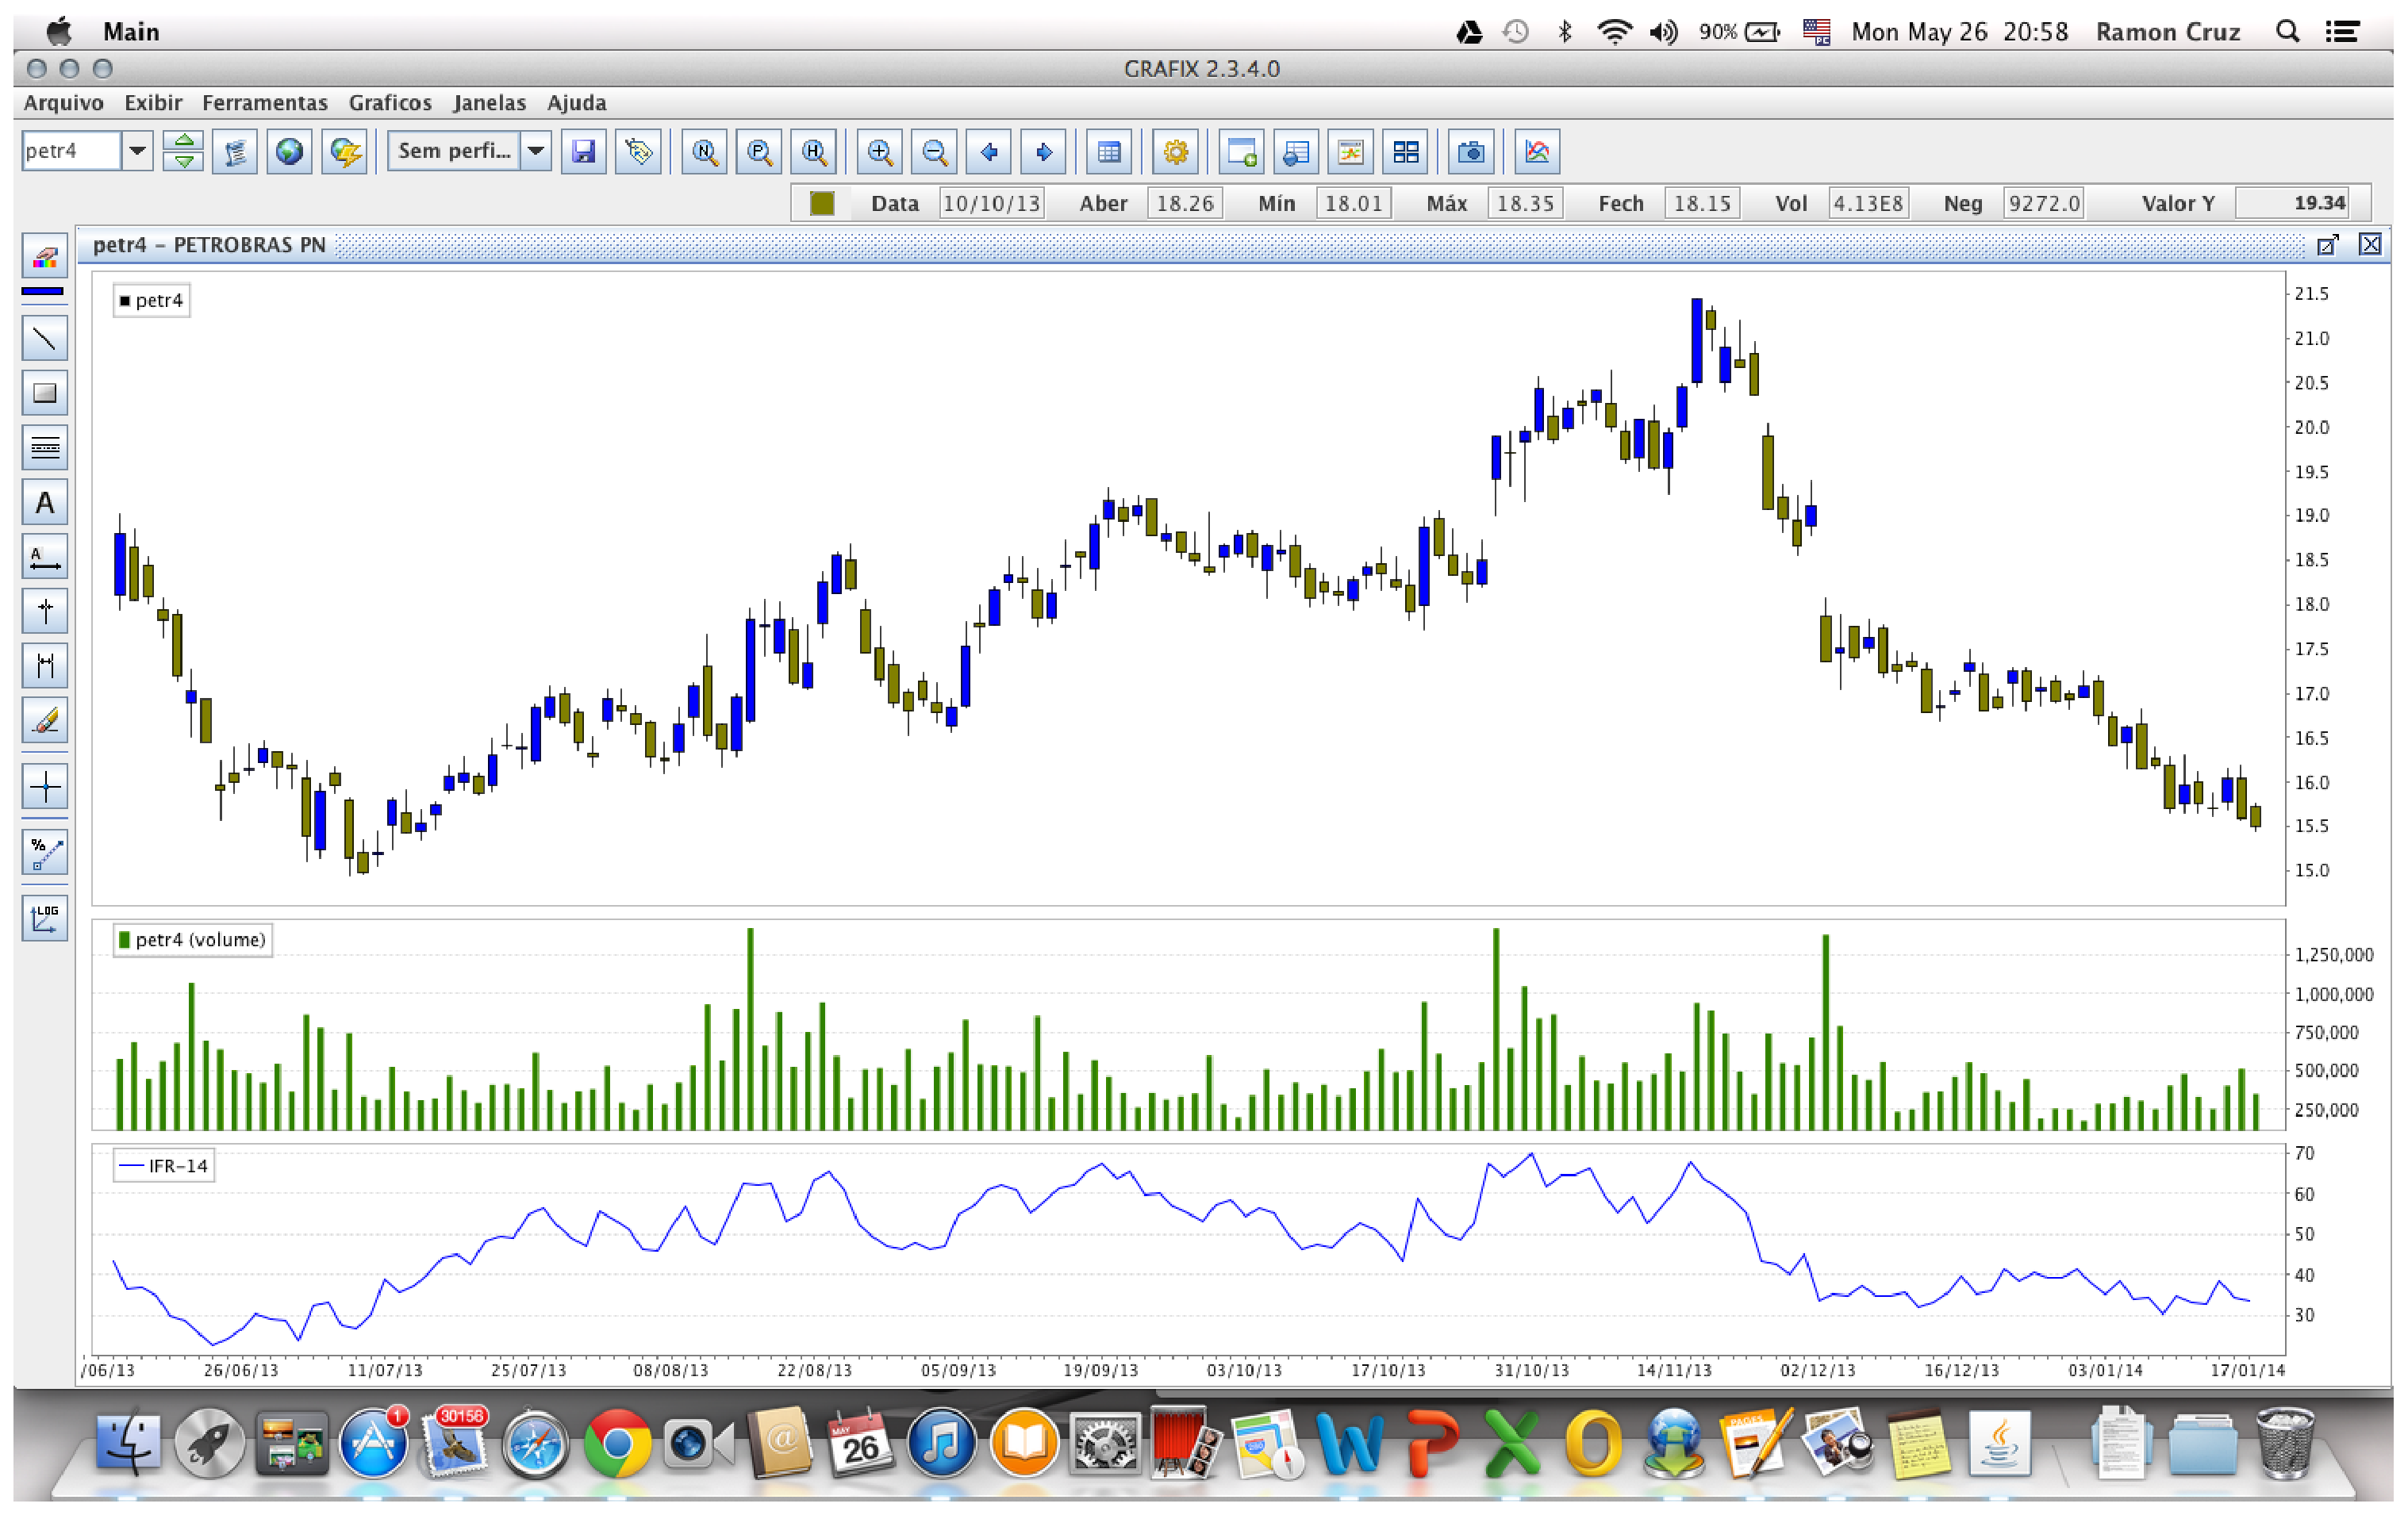
\includegraphics[width=0.5\textwidth]{figuras/f05}
\caption{Grafix}

\end{figure}

\section{Engenharia de Software}
\subsection{Mode-View-Controller (MVC)}

Segundo Krasner e Pope (\citeyear{krasner1988}), quando construímos produtos de Software modularizando seus componentes, obtemos bons resultados. Isolar funcionalmente cada unidade permite aos desenvolvedores entenderem e modificarem mais facilmente cada unidade, sem que seja necessário conhecer todas as unidades envolvidas no Software em questão. Desta forma, uma arquitetura modularizada de um Software contribui para atividades de manutenção e evolução deste, tornando-as mais fáceis \cite[p. 1]{krasner1988}.


A arquitetura Model-View-Controller (MVC) concentra-se nos três módulos: (i) Model, é a representação o conhecimento que pode ser composto por um ou vários objetos; (ii) View, é a representação visual da Model, ou seja, é através da View que o usuário tem acesso às informações da Model; (iii) Controller, permite a associação entre Models e Views, com entradas de dispositivos (i.e. teclados, mouses, entre outros)\cite[p. 2]{krasner1988}.



Para manter todas as Views e Controllers cientes das mudanças de estado ocorridas na Model, foi desenvolvida também a noção de dependência. Nesse contexto, os objetos do tipo Controller e View são registrados em uma lista de dependentes na Model, e quando ocorre alguma mudança, estes são avisados através de troca de mensagens \cite[p. 2]{krasner1988}, como ilustra a figura 6. No capitulo 5, encontra-se uma explanação da aplicação do MVC na ferramenta proposta.

\begin{figure}[h]
\centering
\label{f06}
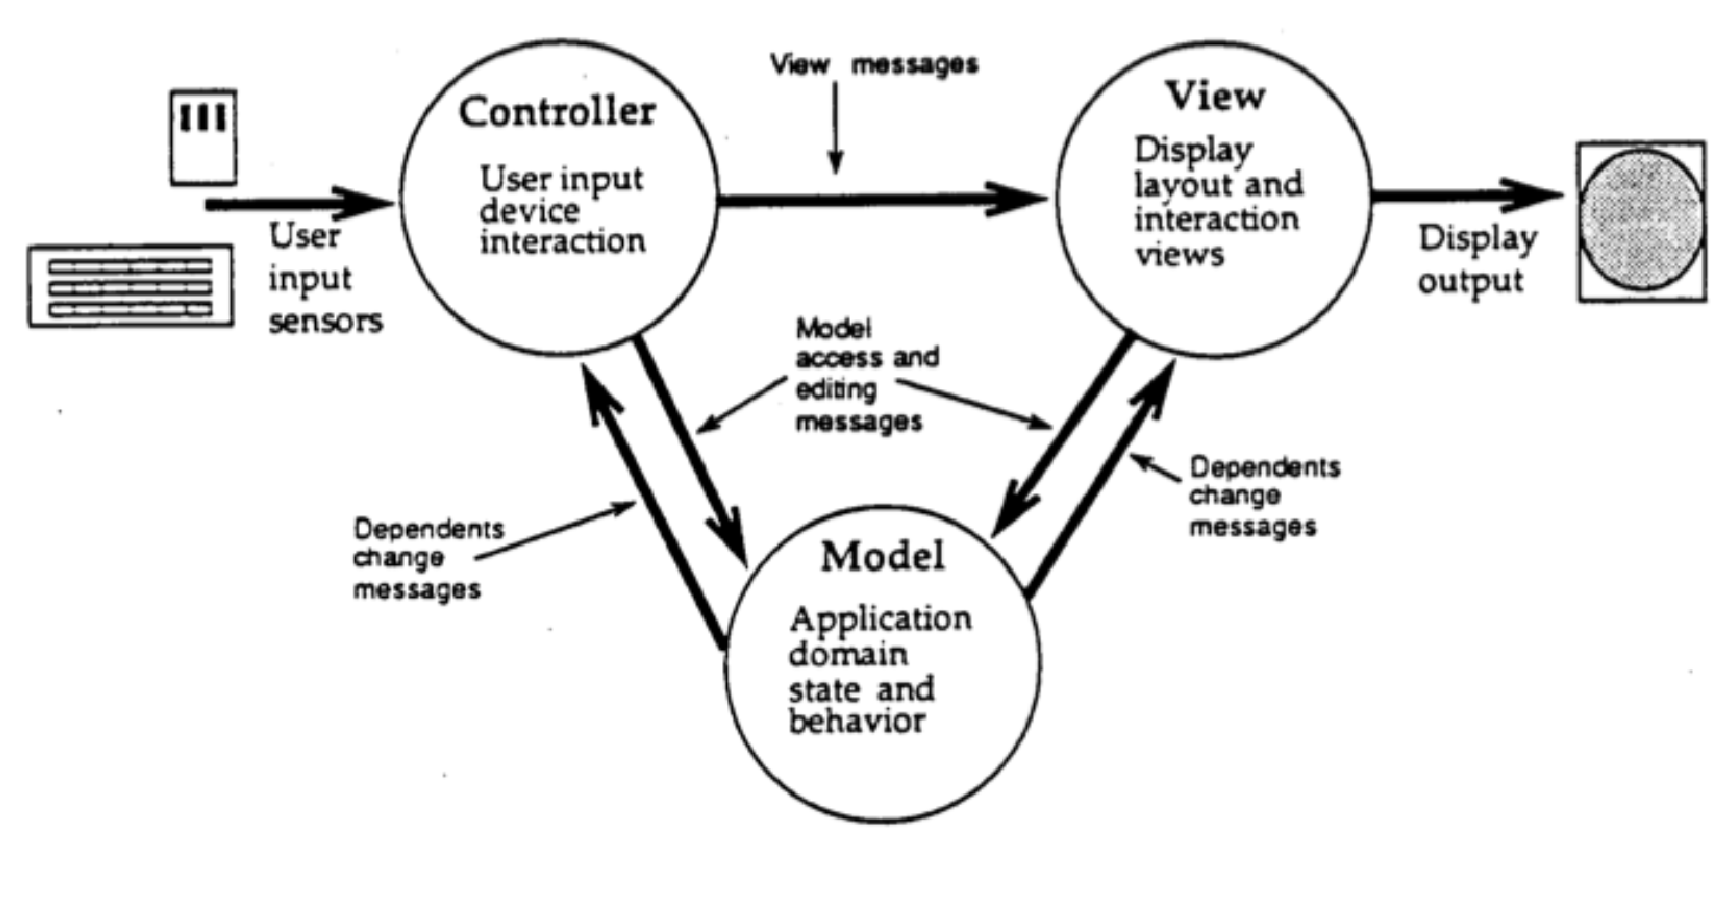
\includegraphics[width=1\textwidth]{figuras/f06}
\caption{Model-View-Controller e o envio de mensagens}

\end{figure}



\subsection{Padrões de Projeto}

Christopher Alexander afirma que \apud[p.19]{christopher1977}{gamma2000}, \textit{“cada padrão descreve um problema no nosso ambiente e o cerne da solução, de tal forma que você possa usar essa solução mais de um milhão de vezes, sem nunca fazê-lo da mesma maneira”}. Apesar do contexto de Alexander ser o da arquitetura, suas colocações aplicam-se no contexto de desenvolvimento de Software orientado a objetos. O núcleo de ambos os tipos de projetos é a solução para um problema num determinado contexto \cite[p.19]{gamma2000}.

No contexto de Software, de acordo com Gamma (\citeyear{gamma2000},p.20): \textit{“Um padrão de projeto nomeia, abstrai e identifica os aspectos-chave de uma estrutura de projeto comum para torná-la útil para criação de um projeto orientado a objetos reutilizável”}. Cada padrão de projeto tem como objetivo solucionar um problema em particular. Para Gamma, um padrão de projeto tem quatro elementos essenciais: (i) Nome do padrão, descreve o problema em uma ou duas palavras; (ii) Problema, descreve a aplicação do projeto; (iii) Solução, descreve os elementos que compõe um projeto, seus relacionamentos, responsabilidades e colaborações; (iv) Consequências, descreve as vantagens e desvantagens de cada padrão \cite[p.19]{gamma2000}.

\subsubsection{Padrões de projeto adotados neste TCC}

\subsubsubsection{Strategy}

Trata-se de um padrão comportamental, o qual permite a variação de algoritmos, independentemente dos clientes que os usam, facilitando ainda ser sensível ao contexto. O Strategy é composto por três participantes: (i) Context, é quem chama uma estratégia através de uma entidade do tipo interface; (ii) Strategy, é a interface comum a todos os algoritmos relacionados à ela; e (iii) Concrete Strategy, é a classe concreta que implementa os diferentes algoritmos \cite[p.294]{gamma2000}. 

Como o padrão Strategy delega a implementação de algoritmos às classes concretas bem como se baseia na implementação usando entidades do tipo interface, esse padrão oferece maior facilidade na manutenção de Software, em especial na manutenção evolutiva do mesmo. A figura 7  ilustra a arquitetura básica deste padrão \cite[p.295]{gamma2000}. Durante o desenvolvimento da ferramenta proposta, outros padrões de projetos foram adotados, conforme a necessidade.

\begin{figure}[h]
\centering
\label{f07}
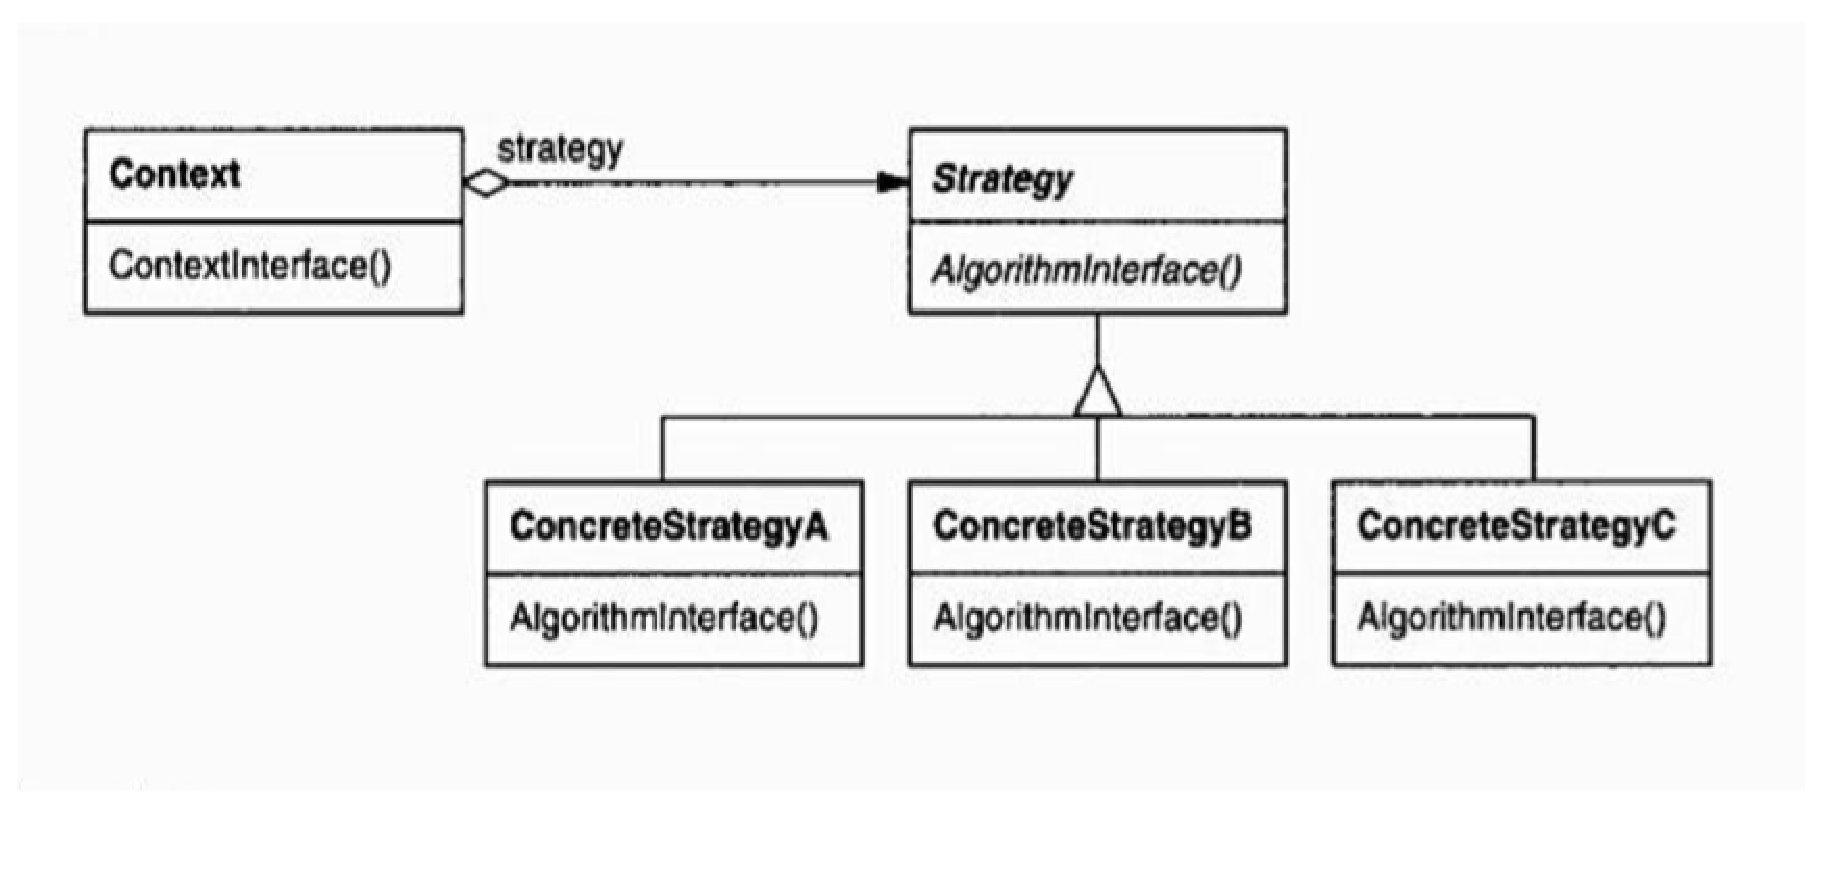
\includegraphics[width=0.9\textwidth]{figuras/f07}
\caption{Padrão Strategy}
\end{figure}
\subsubsubsection{Singleton}

Trata-se de um padrão de criação, cujo objetivo é garantir que uma classe possua somente uma instância e tenha ainda um ponto global de acesso à essa instância. Gamma (\citeyear{gamma2000}, p. 130) ilustra um cenário de aplicação deste padrão. Este cenário contém um sistema onde existem várias impressoras e deveria haver somente um \textit{spooler} (i.e. arquivo temporário que concentra os demais arquivos a serem impressos). Da mesma forma, deve haver somente um sistema de arquivos e um gerenciador de janelas. Neste cenário, nota-se a necessidade em garantir que a classe que detem o controle do \textit{spooler} tenha apenas uma instância. E tenha ainda, um ponto público de acesso a essa instância. Gamma (\citeyear{gamma2000}, p. 130) afirma que, a melhor solução seria tornar a própria classe responsável por manter o controle da sua única instância. A classe pode garantir que nenhuma outra instância seja criada, bem como pode fornecer um meio para acessar sua única instância. Este é o padrão Singleton.

\begin{figure}[h]
\centering
\label{f08}
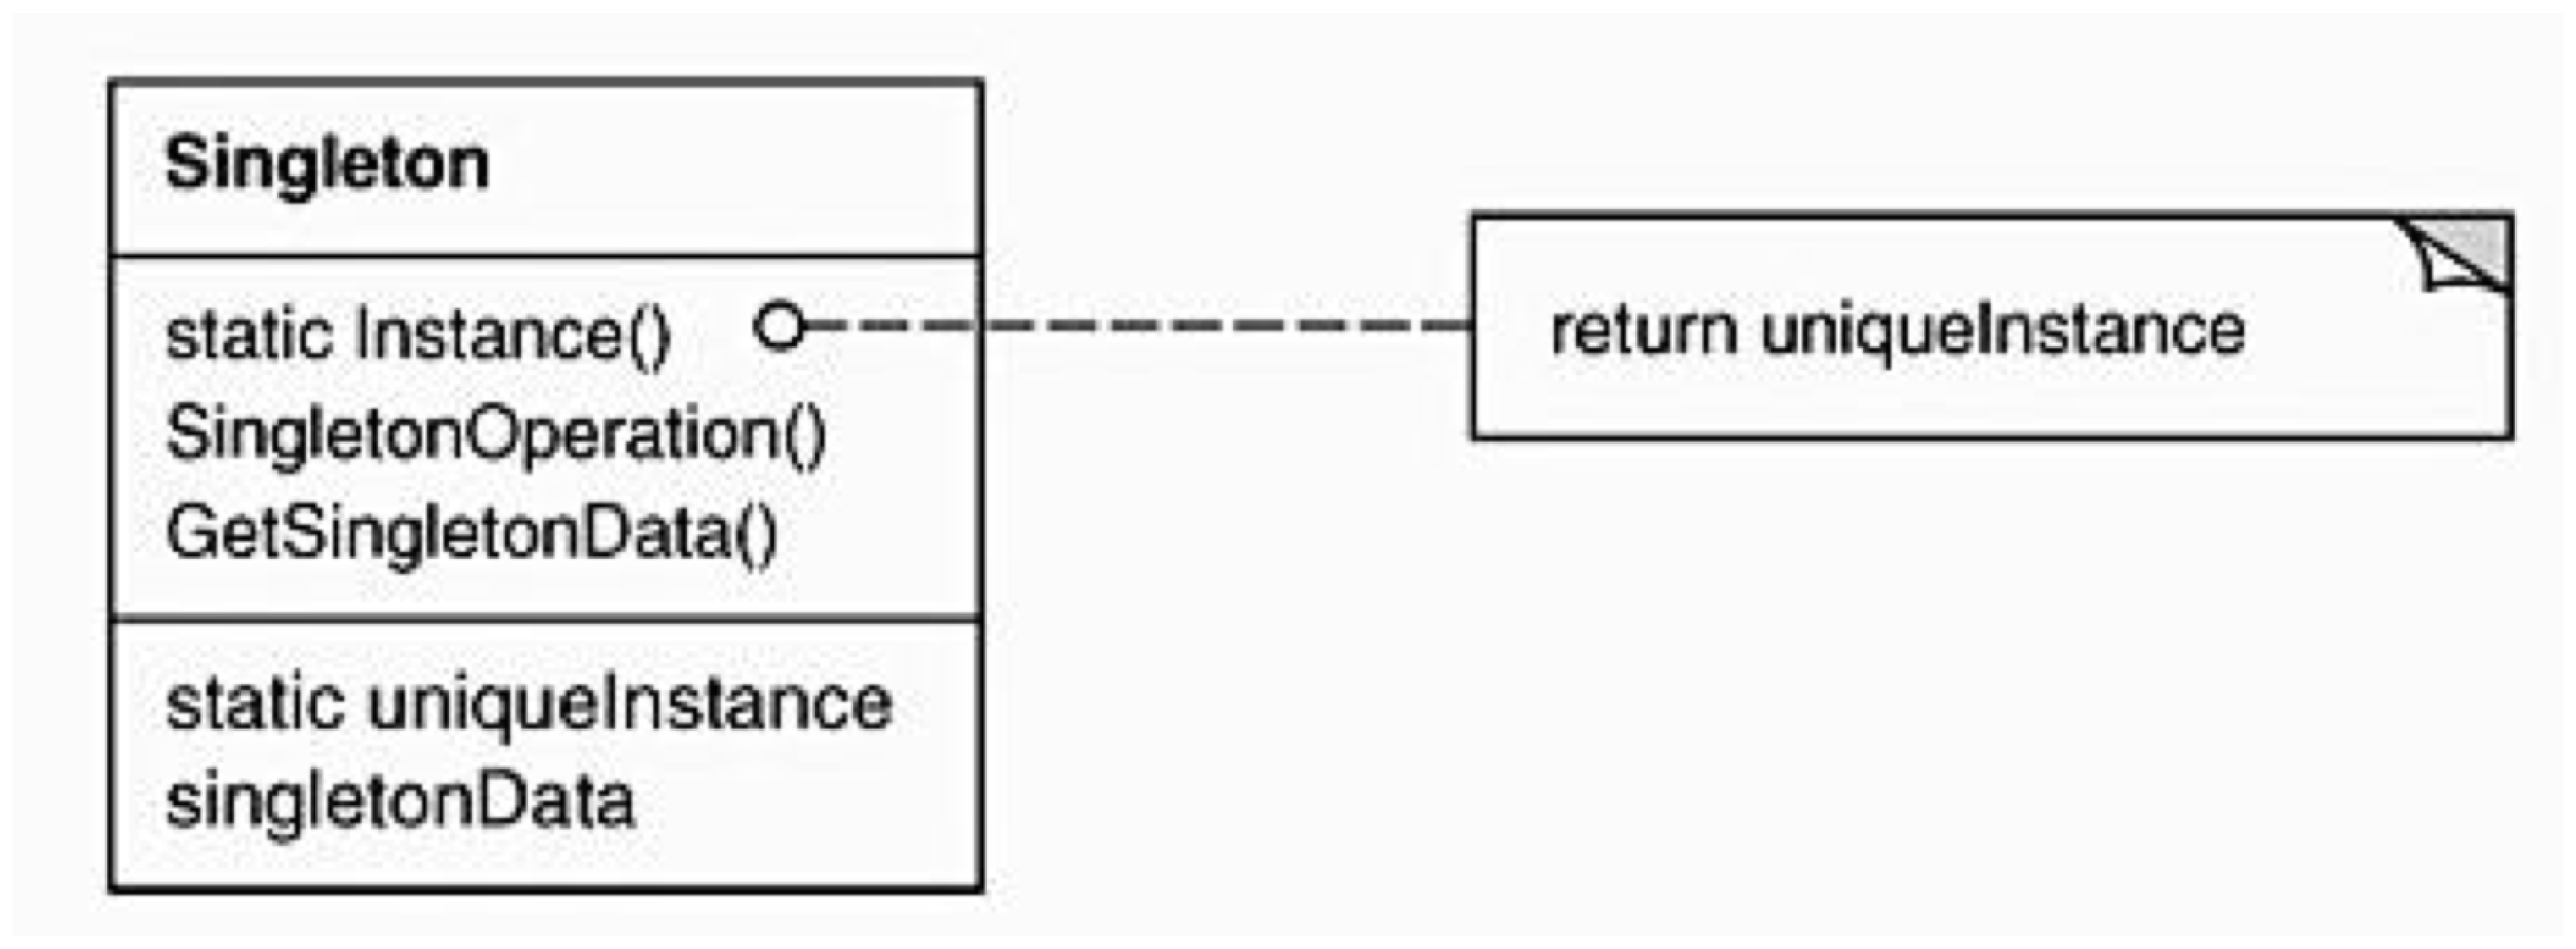
\includegraphics[width=0.9\textwidth]{figuras/singleton}
\caption{Padrão Singleton}
\end{figure}

A figura 8 ilustra uma classe que implementa o padrão Singleton. Esta classe possui o método estático Instance(), que é a única forma de acessar a instância criada por esta classe.


\subsubsubsection{DAO - Data Access Object}

Trata-se de um padrão estrutura, cujo propósito é isolar a camada de modelo da camada de persistência. Dessa maneira, obtém-se como benefícios a simplificação da manutenção da camada de persistência,  organização na forma de prover e requisitar informações localizadas na base de dados, e baixo acoplamento. A figura 9 apresenta as classes participantes no padrão DAO, tais como: (i) BusinessObject, representa as classes da camada modelo; (ii) DataAccessObject, representa as classes principais deste padrão. Elas abstraem os acessos aos dados para as classes do tipo BusinessObject e permitem o acesso transparente à fonte de dados; (iii) DataSource, representa as classes que implementam o acesso aos dados na base de dados do sistema; e (iv) TransferObject, representa os objetos utilizados na comunicação entre as classes DataAccesObject e BusinessObject, \cite{oracle2015}.

\begin{figure}[h!]
\centering
\label{f09}
\includegraphics[width=0.9\textwidth]{figuras/dao}
\caption{Padrão DAO.}
\end{figure}


\subsection{JADE (Java Agent Development Framework)}

O JADE \cite{telecon2014} é um framework implementado em Java que possibilita a programação de Sistemas Multiagentes complexos. O JADE oferece suporte para testes de atividade de debug, arquitetura bem estabelecida para criação, comunicação, identificação, gerenciamento e demais ações com vários agentes atuando como em uma sociedade real. No JADE, os agentes podem trocar mensagens entre si, caracterizando sua arquitetura de comunicação como troca de mensagem. Este framework foi desenvolvido de acordo com as especificações Foundation for IntelligentPhysicalAgents (FIPA) \cite{telecon2014}, que é uma comunidade IEEE que promove padrões tecnológicos para Sistemas Multiagentes. Por ter sido implementado integralmente em Java, o JADE pode ser executado em qualquer sistema operacional que possua uma Máquina Virtual Java.

O JADE é um Software livre e distribuído pela Telecom Itália, empresa proprietária da TIM Brasil, e possui a Licença LGPL \cite{telecon2014}. Ele é supervisionado por um grupo de empresas de cinco membros: Telecom Itália, Motorola, Whitestein Technologies AG, ProfactorGmbH e France Telecom R\&D. Atualmente, a versão disponível é a 4.3.2, publicada em 28 de março de 2014.

\begin{figure}[h]
\centering
\label{f10}
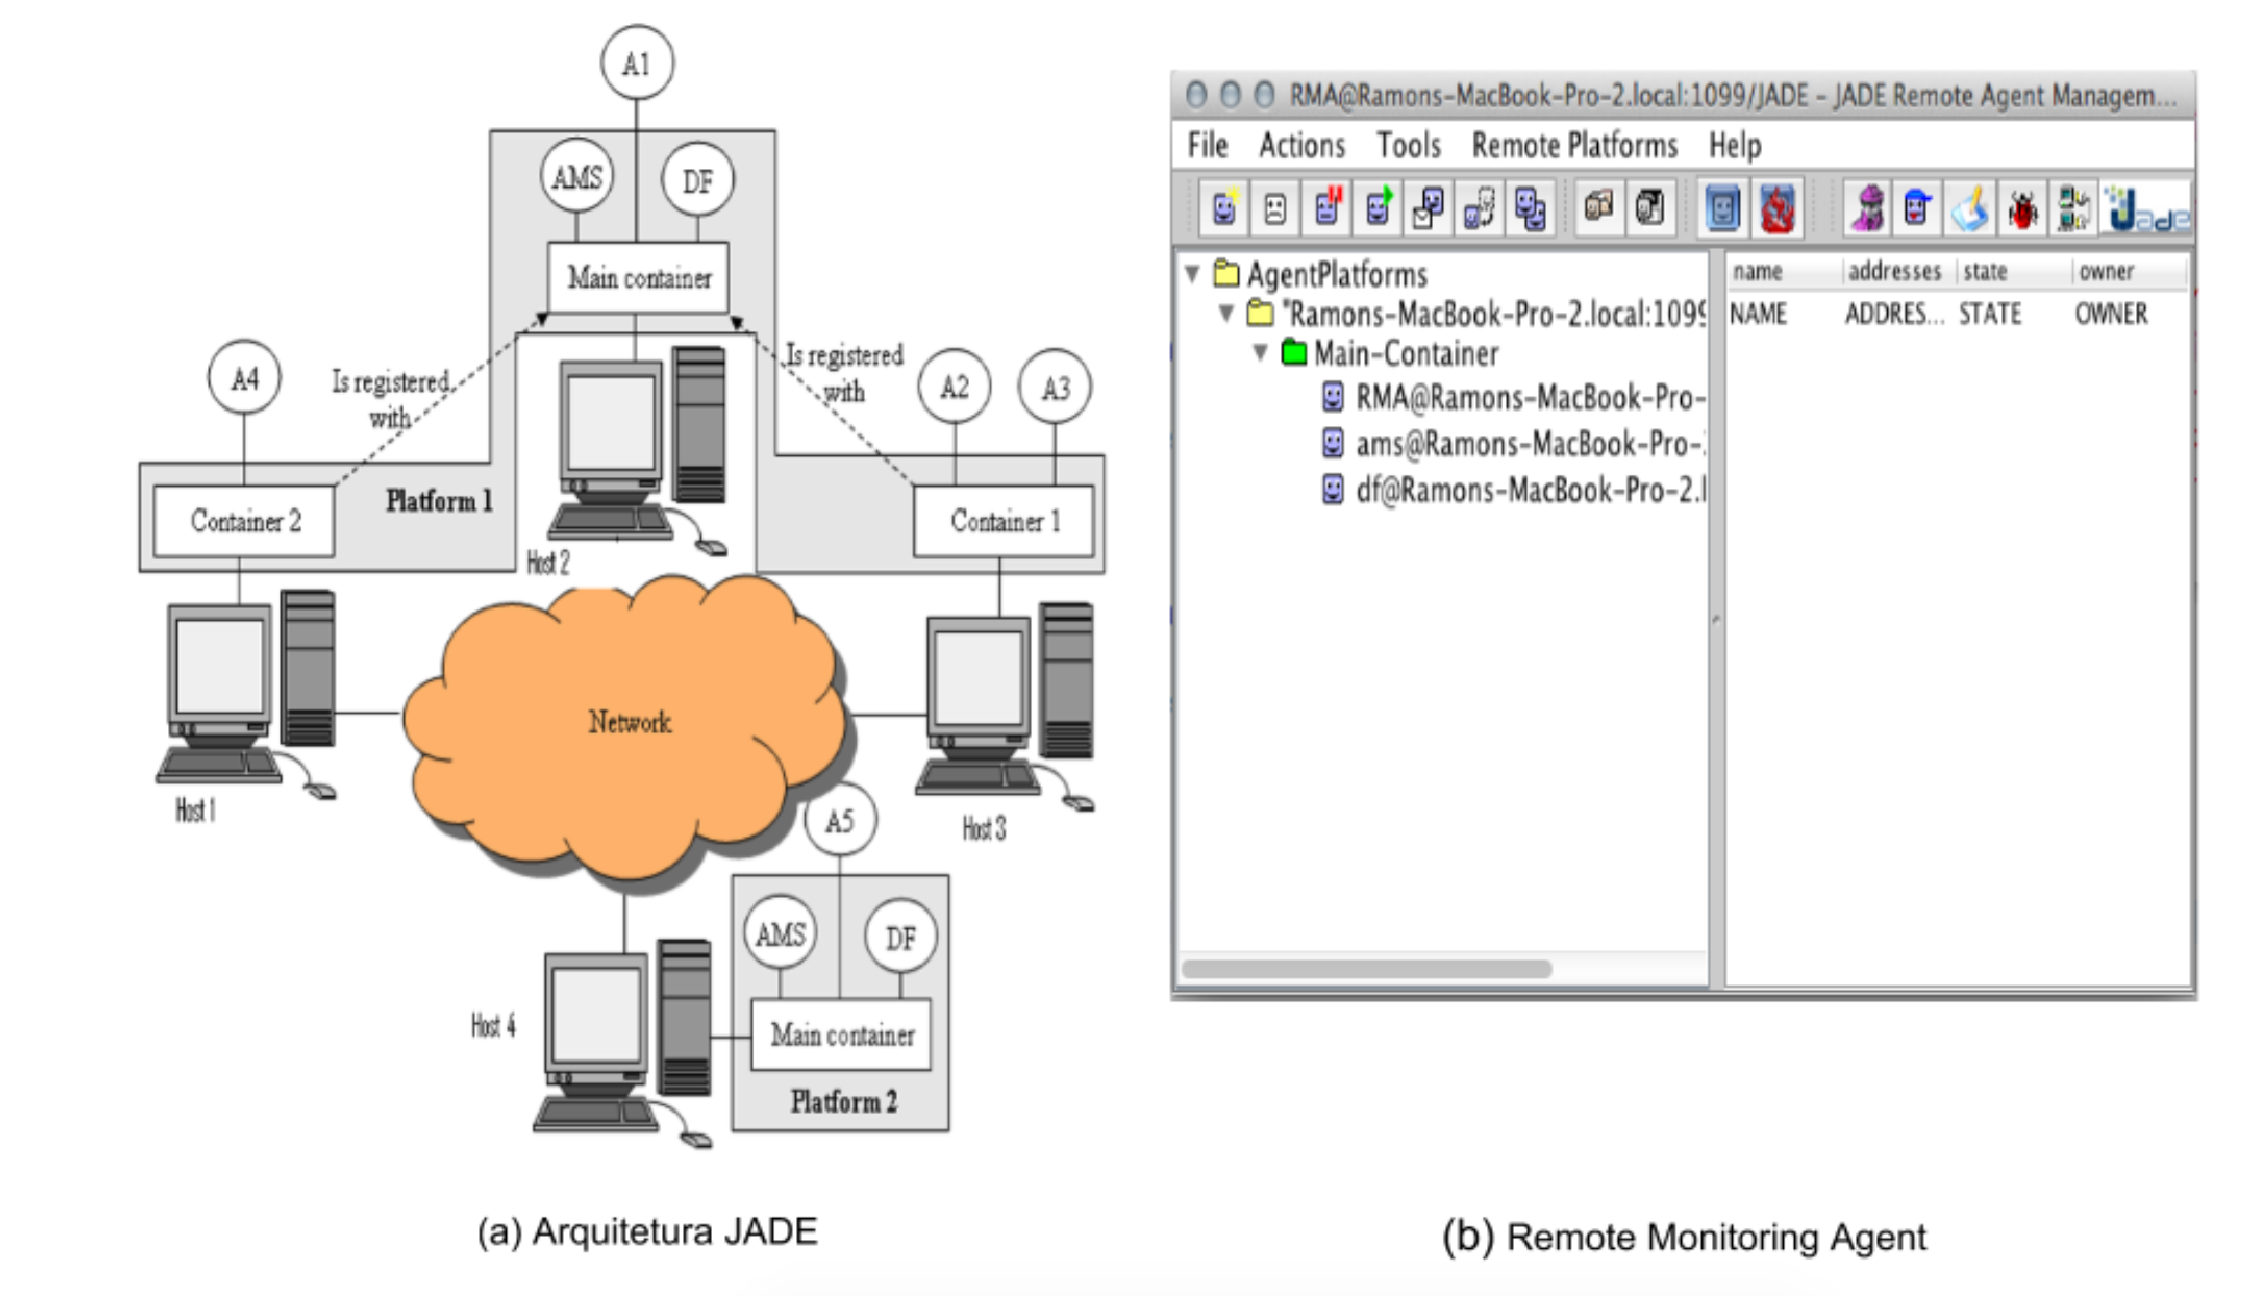
\includegraphics[width=0.9\textwidth]{figuras/f08}
\caption{Arquitetura JADE}

\end{figure}


Considerando a Arquitetura da Plataforma JADE apresentada na figura 8.a, cada Agente instanciado fica contido em um Container, sendo que este pode ter um ou vários agentes. Existem dois tipos de containers, o main e o padrão. O main container contém, por padrão, três agentes: (i) Agente DF (Directory Facilitator), agente responsável por prover serviços, conhecidos no JADE como páginas amarelas, nos quais um dado agente pode encontrar outros agentes, iniciar comunicação com terceiros e registrar/cadastrar os serviços que presta a terceiros; (ii) Agente AMS (Agent Management System), agente responsável por prover serviços de páginas brancas, sendo capaz de criar e excluir agentes em containers remotos ou locais, gerenciando o ciclo de vida dos agentes na plataforma como um todo; e (iii) Agente RMA (Remote Monitoring Agent) (figura 8.b), agente responsável por gerenciar as consoles gráficas providas pela Plataforma JADE.

Simplificadamente, na Arquitetura do JADE, uma dada plataforma é composta por um ou vários containers. Estes containers podem estar em um computador ou distribuídos em uma rede de computadores, como ilustrado na figura 8a. A arquitetura JADE possibilita ainda a comunicação entre os agentes independentemente do container onde estes se encontram, ou seja, o agente A2 pode se comunicar com o agente A3, assim como pode se comunicar também com o agente A5, o qual está em outro container, em outra plataforma, porém conectado a uma rede de computadores. Adicionalmente, serviços, conteúdos e servidores podem ser compartilhados usando como base essa rede de computadores, permitindo aos agentes trabalharem de forma colaborativa, conquistando objetivos até mesmo não triviais, centrados no princípio Dividindo para Conquistar. Princípio esse oriundo de contextos político-sociais bem como amplamente utilizado na atualidade, na ciência da computação como um todo, como uma técnica capaz de lidar com problemas complexos, dividindo esse problema em instâncias menores, resolvendo essas instâncias isoladamente e agrupando os resultados para atingir uma conquista maior, ou seja, a solução do problema de maior complexidade.


\subsection{Metodologia Scrum}

O termo Scrum  é originário do Rugby, esporte criado na Inglaterra. No Scrum, são feitas entregas contínuas de pequenas partes funcionais do Software. O Scrum consiste em times associados a papéis, eventos, artefatos e regras. Cada componente tem uma função específica no desenvolvimento do Software \cite{schwaber2013}.

O time Scrum é formado por:(i)um Scrum Master, que é a figura do líder do time. Ele é o responsável por fazer o time compreender as regras do Scrum; (ii) um grupo de desenvolvimento (time), que são os programadores, designers, entre outros; e (iii) um Product Owner, que é uma pessoa com bom conhecimento das necessidades do produto. No Scrum, os times são auto-organizáveis no que tange à escolha da melhor forma para realizar um trabalho. O modelo de time no Scrum foi pensado de forma que valorize a flexibilidade, criatividade e produtividade.  O time entrega produtos de forma iterativa e incremental, assim aumentando oportunidades de \textit{feedback} contínuo. Estas entregas são versões parciais funcionais do Software trabalhado pelo time \cite[p. 5-7]{schwaber2013}.

Cada evento no Scrum é uma oportunidade de verificar e corrigir algo no produto. Eles são projetados para que seja possível obter transparência e uma inspeção criteriosa do produto. Cada evento termina sempre que seu objetivo é alcançado. No Scrum, o evento principal é a Sprint. Ela é o ciclo de desenvolvimento do produto, que dura um mês ou menos, sendo composta por:(i) uma reunião de planejamento; (ii) reuniões diárias curtas; (iii) uma revisão da Sprint, (iv) uma retrospectiva; e o  (v) trabalho de desenvolvimento do produto.

Segundo Schwaber e Sutherland (\citeyear{schwaber2013}, p.13), \textit{“Os artefatos do Scrum representam o trabalho ou o valor para o fornecimento de transparência e oportunidade para inspeção e adaptação.”} Os artefatos são elaborados de forma que o entendimento das informações contidas nele seja o maior possível. Dentre os artefatos do Scrum temos: (i) Backlog do Produto, é uma lista de tudo que é necessário no produto. Ela é a origem dos requisitos e é gerida pelo Product Owner. O Backlog do Produto é dinâmico e existe enquanto houver o produto; (ii) Backlog da Sprint, é o conjunto de itens selecionados do Backlog do Produto para a Sprint, ou seja, é o conjunto de características que serão implementadas pelo time durante a Sprint; (iii) Incremento, é a soma de todos os itens do Backlog do Produto entregues no final de uma Sprint \cite[p. 13-15]{schwaber2013}. 


\section{Resumo do Capítulo}

Elucidou-se nesse capítulo, no Contexto Financeiro, uma breve exposição de algumas ferramentas de análise técnica comumente encontradas no Mercado Financeiro para apoiar o investidor. Destaca-se nelas uma característica em comum, que é a necessidade de seu usuário possuir conhecimentos relacionados à análise técnica. 

Na Engenharia de Software, foi apresentado um modelo arquitetural bastante aceito, o Model-View-Controller. Este modelo concentra-se na divisão da arquitetura de um Software em três módulos autônomos que se comunicam entre si. Foram apresentados ainda os padrões de projeto: (i) Strategy, (ii) Singleton, e (iii) DAO. Adotados neste TCC. 

Adicionalmente, foi descrito o framework JADE, o qual foi adotado neste TCC para implementar os agentes comportamentais planejados para o desenvolvimento da ferramenta. E por fim, foi apresentada a metodologia Ágil, que foi adaptada para conduzir o desenvolvimento da ferramenta acordada por este TCC.

\newpage
\FloatBarrier
\chapter[METODOLOGIA]{Metodologia}

Neste capítulo, serão apresentadas as principais metodologias de pesquisa científica encontradas na literatura. Em um segundo momento, será especificada qual a metodologia de pesquisa científica, dentre as pesquisadas, que mais se adequou ao tema coberto nesse Trabalho de Conclusão de Curso. Posteriormente, são descritas: (i) a metodologia utilizada para condução do Trabalho de Conclusão de Curso como um todo, da atividade de levantamento de referencial teórico à escrita final do trabalho, chamada macro metodologia. Ainda nessa seção, será descrita a atividade de desenvolvimento de provas de conceito, a qual foi de suma importância para definir o suporte tecnológico adequado ao desenvolvimento da ferramenta; (ii) a metodologia que conduziu o desenvolvimento da ferramenta em si, e (iii) a metodologia que orientou a análise dos resultados obtidos.

\section{Metodologias de Pesquisa Científica}

Segundo Gil (\citeyear{gil2002}, p.17), pode-se definir pesquisa como o procedimento racional e sistemático que tem como objetivo proporcionar respostas aos problemas que são propostos. Gil afirma ainda, que é usual classificar uma pesquisa com base em seus objetivos gerais. Assim, uma pesquisa pode ser classificada em três grupos: (i) exploratórias; (ii) descritivas; e (iii) explicativas. \cite[p. 41]{gil2002}.

As pesquisas exploratórias têm como objetivo principal buscar familiaridade com o problema abordado, de maneira a aprimorar ideias.  Pesquisas exploratórias possuem um planejamento mais flexível. Entretanto, na maioria dos casos assume a forma de pesquisa bibliográfica ou de estudo de caso. \cite[p. 41]{gil2002}.

As pesquisas descritivas têm como objetivo principal descrever características de determinada população, fenômeno, ou a descrição de relações entre variáveis. Segundo Gil (2002, p.42), as pesquisas descritivas e as exploratórias são habitualmente realizadas por pesquisadores sociais preocupados com a atuação prática e, geralmente, assumem a forma de levantamento.

As pesquisas explicativas têm como objetivo principal a identificação dos fatores que determinam ou contribuem para ocorrência de um determinado fenômeno. De acordo com Gil (\citeyear{gil2002}, p.42), esse é o tipo de pesquisa mais complexo e delicado, pois é exigido um profundo conhecimento da realidade. No entanto, isso não significa que as pesquisas exploratórias e descritivas tenham um valor inferior. Estas, geralmente, constituem uma etapa prévia indispensável para que se possa obter explicações científicas. 

O levantamento acordado anteriormente procura classificar a pesquisa científica quanto aos seus objetivos. Com base no tipo de pesquisa científica, algumas metodologias podem ser mais adequadas do que outras. Por exemplo, caso a pesquisa seja de cunho exploratório, cabe a utilização de uma metodologia de pesquisa científica exploratória. 

Adicionalmente, uma pesquisa pode ser classificada quanto à sua abordagem. Nesse caso, uma pesquisa pode ser quantitativa (aplicada quanto se pode mensurar os dados analisados), qualitativa (quando os dados analisados são subjetivos) ou híbrida. Nesse último caso, a abordagem envolve ambas as análises, quantitativa e qualitativa.

\section{Classificação da Pesquisa }

O tipo de pesquisa adotado neste TCC foi o exploratório, cujo objetivo foi explorar o paradigma de Sistemas Multiagentes Comportamentais no contexto Financeiro, especificamente no contexto da Bolsa de Valores de São Paulo. O resultado desta pesquisa foi uma ferramenta de estratégia financeira capaz de abstrair a complexidade de cálculos financeiros comumente utilizados na Análise Técnica. A ferramenta foi projetada de maneira a facilitar a evolução da máquina de raciocínio dos agentes, bem como suas futuras manutenções. 


\section{Metodologia de Condução do Trabalho de Conclusão do Curso}

A realização do TCC foi orientada por uma macro metodologia, a qual foi organizada em atividades.
Essas atividades compreenderam desde "Levantar Referencial Teórico" a "Escrever TCC 02", conforme apresentado na figura 11, modelada no Bizagi \textcopyright.
\begin{figure}[h]
\centering
\label{f11}
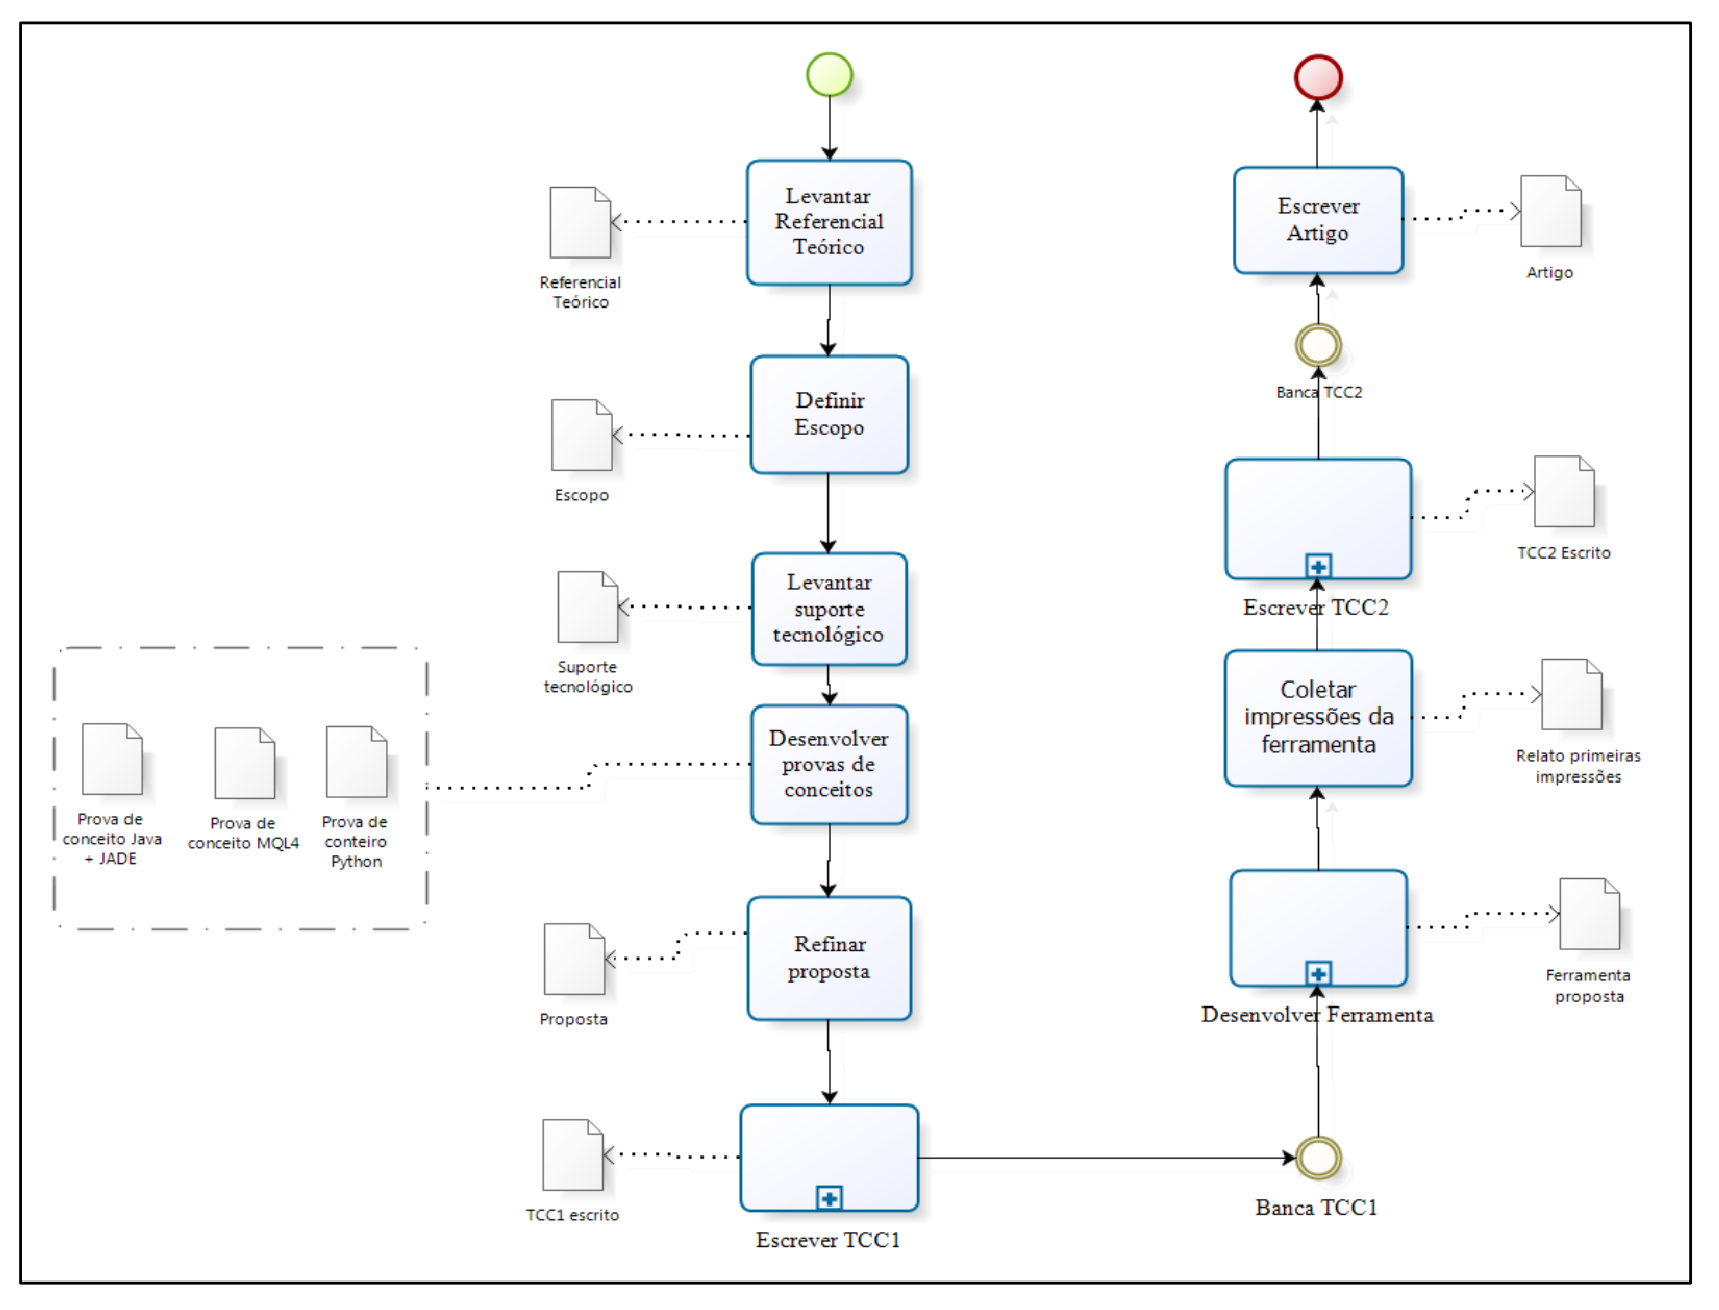
\includegraphics[width=0.9\textwidth]{figuras/f27}
\caption{Desenvolvimento TCC}
\end{figure}
Visando elucidar o que foi realizado em cada atividade, seguem breves descrições sobre essas atividades:

\begin{description}
\item [Levantar Referencial Teórico:] Nesta atividade, foram feitos levantamentos de artigos científicos, artigos jornalísticos, publicações de empresas públicas/privadas, possíveis tecnologias que mais se adequassem ao tema tratado no trabalho, possibilitando maior conhecimento dos domínios Financeiro e de Engenharia de Software.

\item [Definir Escopo]:
Nesta atividade, o escopo do TCC foi definido como sendo "Construir uma Ferramenta de estratégia financeira apoiada por Sistemas Multiagentes Comportamentais".

\item [Levantar Suporte Tecnológico:] 
 Nesta atividade, foram levantadas as tecnologias que mais se adequavam, em um primeiro momento, ao tema coberto no TCC.

\item [Desenvolver Provas de Conceito:]
Nesta atividade, foram implementadas provas de conceito, utilizando uma adaptação da metodologia Scrum, em diferentes suportes tecnológicos, visando à definição de uma boa estratégia em atendimento à ferramenta.

\item [Refinar Proposta:] 
Nesta atividade, foi feita uma revisão da proposta quanto ao Referencial Teórico, ao Suporte Tecnológico bem como outros detalhes, em atendimento ao tema do trabalho.

\item [Escrever TCC1:]
Nesta etapa, foi feita a documentação dos resultados obtidos nas etapas anteriores, possibilitando a obtenção da escrita final do TCC01.
\end{description}

Após a avaliação da Banca de TCC1, ajustes foram realizados na parte escrita, no intuito de atender as colocações apontadas pelos membros da Banca. Posteriormente, o TCC foi conduzido considerando as seguintes atividades metodológicas:

\begin{description}
\item [Desenvolver Ferramenta:]
Nesta atividade, foi feito o desenvolvimento da ferramenta utilizando uma adaptação da metodologia Scrum. Os passos metodológicos dessa atividade são descritos na subseção 4.4, ainda neste capítulo.

\item [Coletar Impressões da Ferramenta:]
Um vez desenvolvida a primeira versão da ferramenta, foram conduzidos testes em laboratório bem como junto aos usuários finais da ferramenta. Esses testes possibilitaram análises quantitativas e qualitativas, permitindo ainda a coleta das primeiras impressões da ferramenta. Com base nesses resultados, refinamentos e ajustes foram realizados usando uma abordadem de pesquisa-ação. Parte desses refinamentos foram acordados de forma empírica. Esse processo foi iterativo-evolutivo, sendo realizadas, portanto, algumas iterações até a obtenção da versão atual da ferramenta. Todo esse processo é apresentado em detalhes no capítulo 6 desse documento.

\item [Escrever TCC2:] 
Nesta atividade, foram feitas as subatividades: (i) Revisar e refinar Referencial Teórico; (ii) Documentar o desenvolvimento da ferramenta; (iii) Coletar e analisar as impressões da ferramenta; (iv) Documentar o TCC2, em conformidade com as normas ABNT.

\item [Escrever Artigo:]
Nesta atividade, será elaborada a escrita de um artigo para publicação em eventos relacionados ao desenvolvimento de sistemas multiagentes.
\end{description}

Uma atividade que se destaca dentre as apresentadas foi a atividade intitulada "Desenvolver Provas de Conceito".
Na próxima subseção, serão apresentados detalhes sobre esse desenvolvimento, o qual foi de suma importância para uma visão preliminar da ferramenta e do suporte tecnológico utilizado ao longo do TCC.


\subsection{Atividade Desenvolver Provas de Conceito}

Nesta etapa do TCC, foi elaborado um cenário para avaliar o esforço necessário do autor para implementar um Software nas linguagens Java, Mql4 e Python. Para isso, foram adotadas as seguintes etapas para realizar uma prova de conceito: (i) Elaborar cenário, onde foi eleito um padrão de formação encontrado nos gráficos de candlesticks e foi elaborada uma hipótese inicial; (ii) Selecionar  ativos, onde foram eleitas algumas ações com seus devidos valores históricos para testar os produtos de  Software; (iv) Implementar, onde os algoritmos foram implementados nas três linguagens escolhidas; (v) Analisar resultados, onde foi feita a análise manual dos resultados afim de verificar o grau de acerto. Estas etapas estão descritas nos subtópicos seguintes e ilustradas na figura 12.

\begin{figure}[h]
\centering
\label{f12}
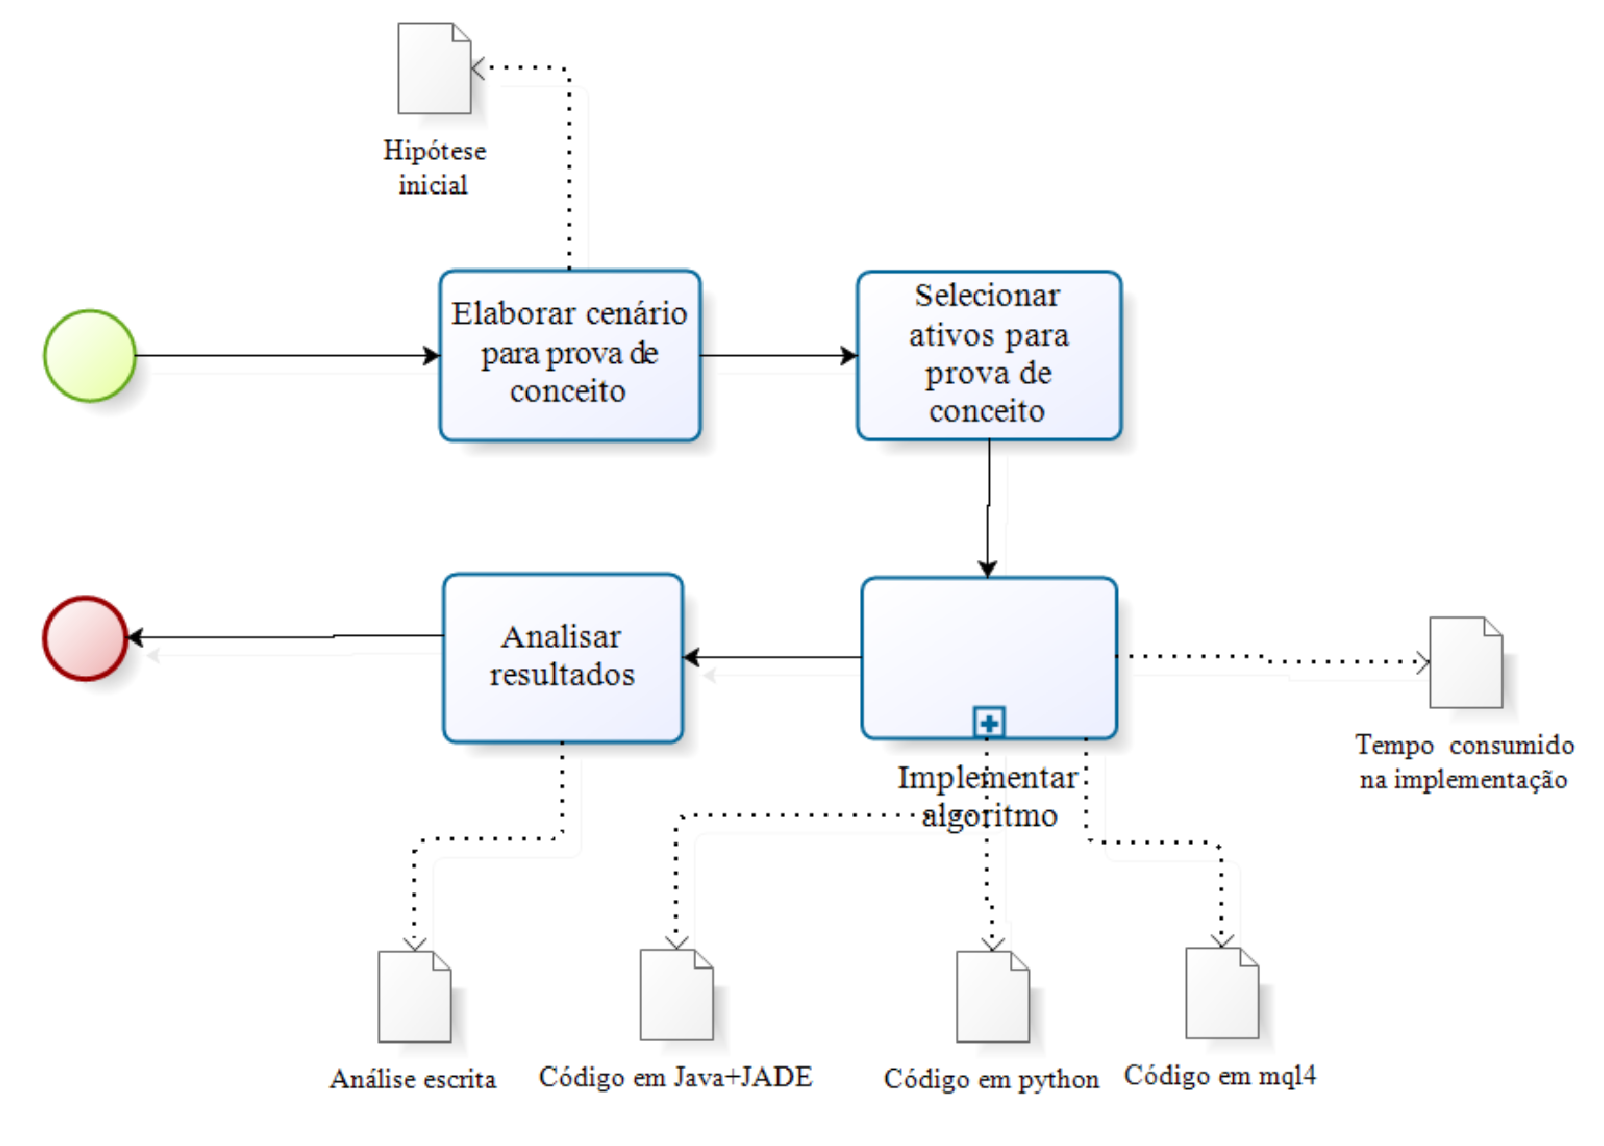
\includegraphics[width=0.9\textwidth]{figuras/f09}
\caption{Processo investigativo }

\end{figure}

\begin{description}
\item [Elaborar Cenário para Prova de Conceito:]
Para nortear as provas de conceito feitas para este estudo, foi elaborado um cenário onde é requerida uma maneira automatizada de se chegar à uma solução. Este cenário é descrito a seguir.

\begin{adjustwidth}{1,5cm}{0cm}
\textit{Uma das maneiras de um investidor acompanhar as movimentações do mercado de capitais, mais especificamente uma Bolsa de Valores, é através de gráficos como: (i) o gráfico de barras ; (ii) o gráfico de linha  e (iii) o gráfico de candlestick\cite[p. 5-6]{matsura2006}. Considerando o último, deseja-se encontrar uma maneira automatizada bem como a formação do padrão de candlestick conhecido como Dark cloud \cite[p.61]{matsura2006}. Padrão este, que poderá compor um plano estratégico de investimento.}

\textit{Uma candlestick é formada por 4 valores: (i) valor de abertura; (ii) valor de máxima; (iii) valor de mínima; e (iv) valor de fechamento. Quando o valor de  fechamento é maior do que o valor de abertura tem-se uma candlestick de alta, quando ocorre o inverso tem-se uma candlestick de baixa. A figura 13 ilustra uma candlestick de alta, que é representada com o preenchimento em branco e uma candlestick de baixa, que é representada com o preenchimento em vermelho. Cada candlestick representa uma periodicidade, a qual pode ser desde um minuto até um ano \cite[p.6]{matsura2006}.}
\end{adjustwidth}

\begin{figure}[h!]
\centering
\label{f13} 
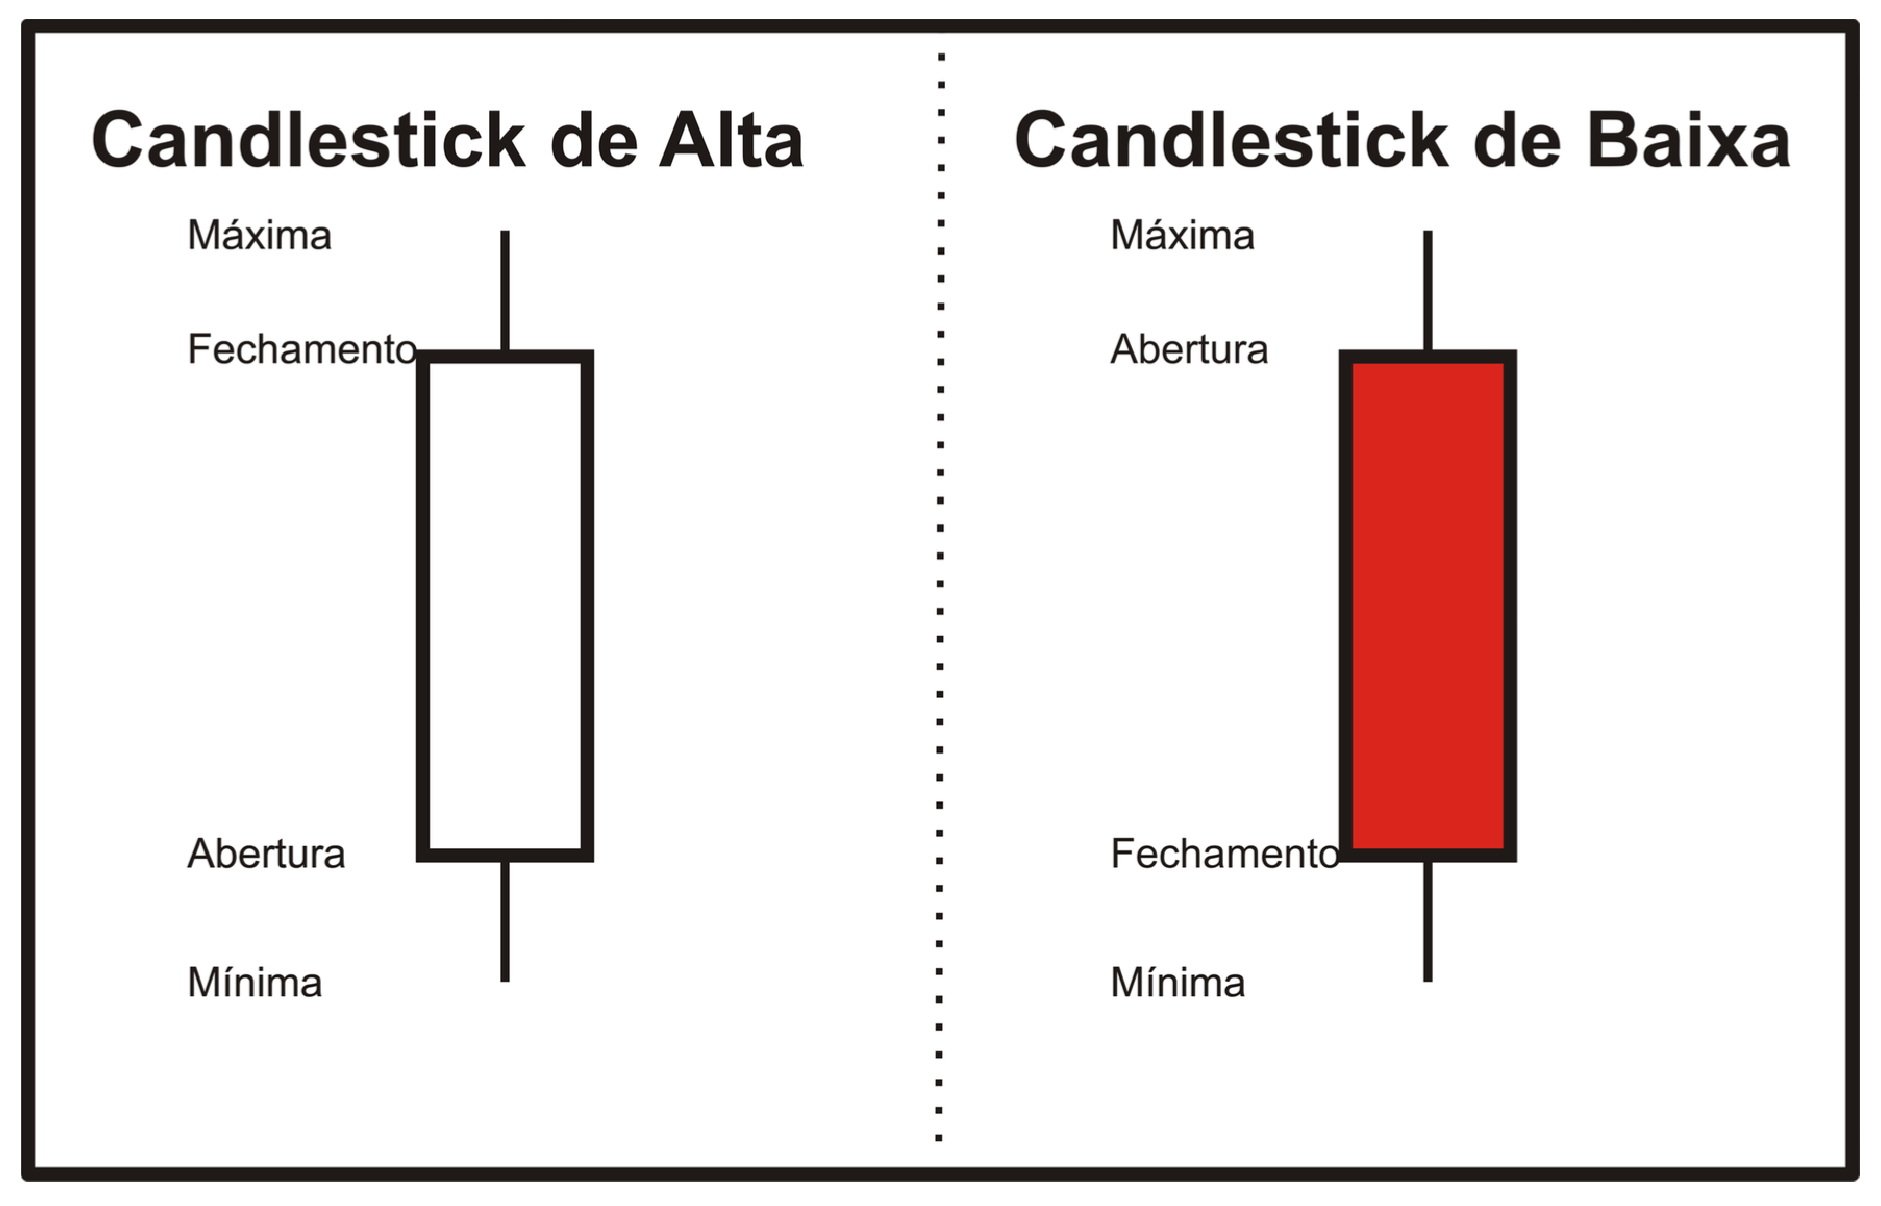
\includegraphics[width=0.8\textwidth]{figuras/f10}
\caption{Candlestick }
\end{figure}

O padrão Darkcloud (figura 14) é formado por duas clandlesticks, sendo a primeira de alta e a segunda de baixa, onde a segunda tem a abertura maior que a máxima da primeira e fechamento maior que a abertura da primeira \cite[p.61]{matsura2006}. Bigalow faz a seguinte interpretação deste padrão.

\begin{citacao}
Após uma forte tendência de alta, a atmosfera está altista. O otimismo está presente. O preço abre com gap para cima. Os vendedores aparecem e empurram os preços de volta para baixo. Finalmente, o preço fecha na ou próximo das mínimas do dia. O fechamento não confirmou a maioria dos ganhos do dia anterior. Os comprados agora estão preocupados. Obviamente observam que a tendência de alta deve se encerrada. Este sinal proporciona uma boa venda a descoberto, com um estope acima da máxima do dia da vela preta (candlestick de baixa) . \newline \cite[p.47]{bigalow2010}

\end{citacao}
\begin{figure}[h]
\centering
\label{f14}
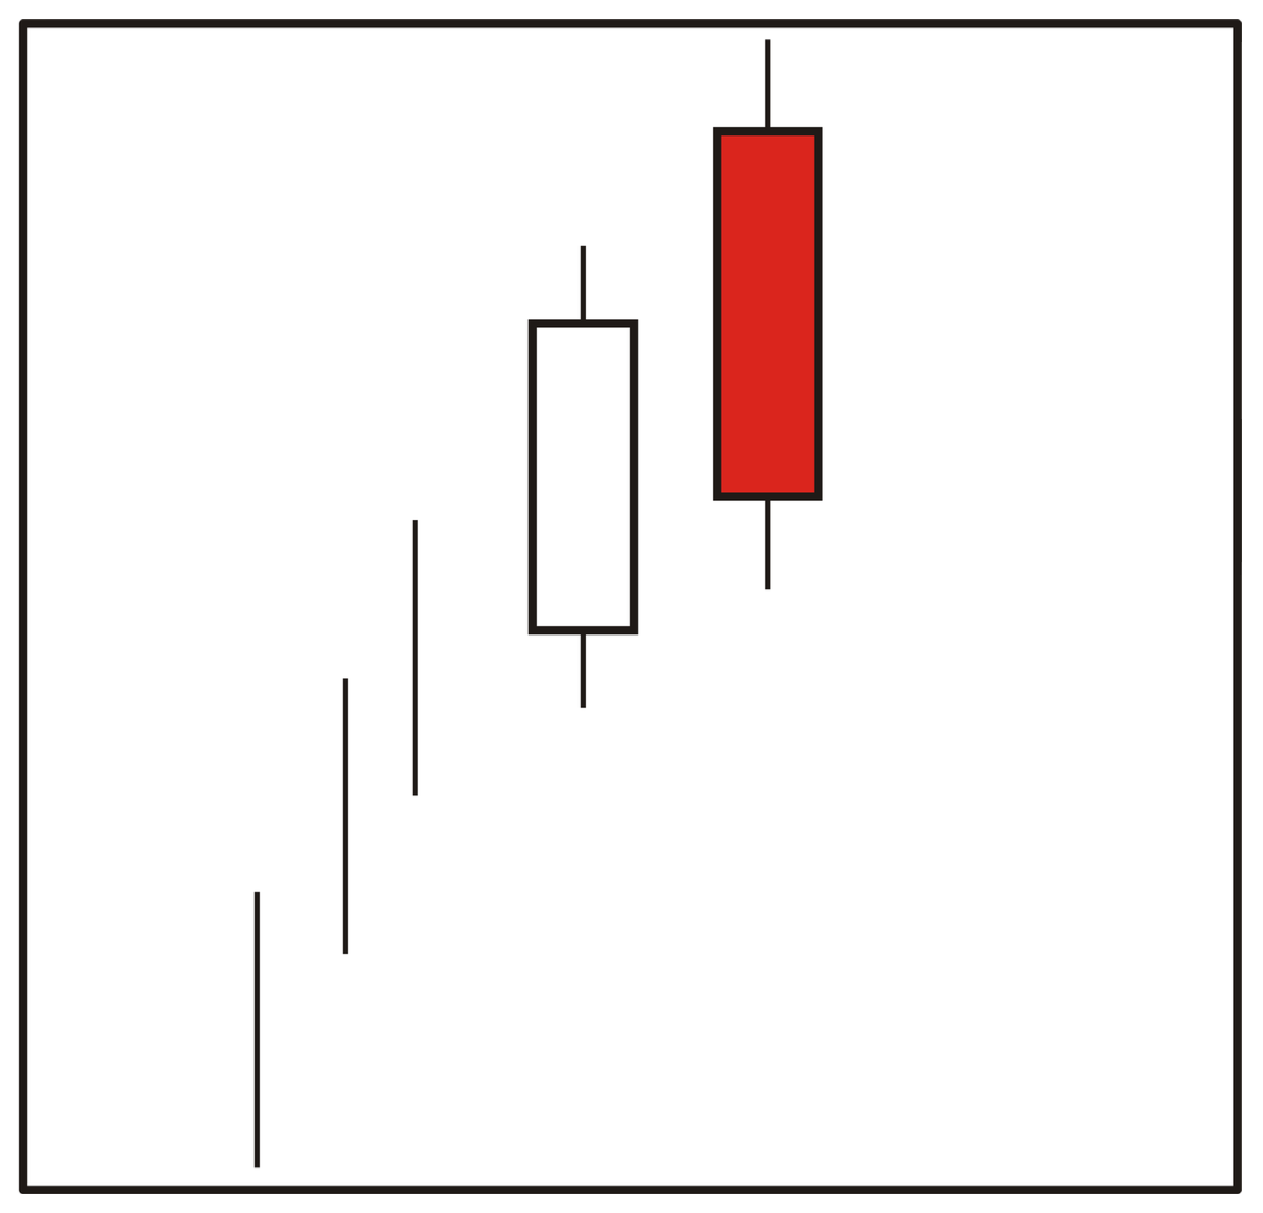
\includegraphics[width=0.5\textwidth]{figuras/f11}
\caption{Padrão DarkCloud}

\end{figure}

Diante deste cenário, criou-se a seguinte hipótese para nortear a atividade: \textit{“A implementação da prova de conceito orientada a Sistemas Multiagentes não será possível ou mesmo demandará muito esforço por parte do desenvolvedor, impossibilitando o seu uso no contexto em estudo neste TCC”}. Iniciaram-se, assim, as outras etapas ilustradas na figura 12.

\item [Selecionar Ativos:]
Nesta etapa, foram obtidos os dados históricos dos ativos (i.e. Ações) das seguintes empresas: (i) Brookfield Incorporações, BISA3.SA; (ii) MVR Engenharia, MRVE3.SA; e (iii) Rossi Residencial S.A., RSID3.SA. Para realizar a atividade com os dados disponíveis aos produtos de Software escritos na linguagem Mql4 \cite{kovalyov2006}, foi feita uma coleta de dados do par de moedas Euro/Dólar americano (EUR/USD). Os códigos Mql4, Java+JADE e Python implementados neste estudo de caso estão disponíveis nos apêndices B, C e D, respectivamente. O período adotado para coleta foi o diário entre fevereiro de 2008 e janeiro de 2014.

\item [Implementar Algoritmo:]
Considere a candlestick de baixa na figura 15 como candlestick 0, e a candlestick de alta como candlestick 1. De acordo com Matsura (\citeyear{matsura2006},p.61), a formação é considerada Darkcloud se:

\begin{itemize}
  \item A candlestick 1 deve ser de alta;
  \item A candlestick 0 deve ser de baixa;
  \item A candlestick 0 deve ter valor de abertura superior ao valor de fechamento da candlestick 1;
  \item A candlestick 0 deve ter seu valor de fechamento entre o valor mediano do corpo da candlestick 1. Deve também ter seu valor de fechamento superior ao valor de abertura da candlestick 1;
  \item A candlestick 0 deve ter um corpo considerável.
\end{itemize}

\begin{figure}[h!]
\centering
\label{f15}
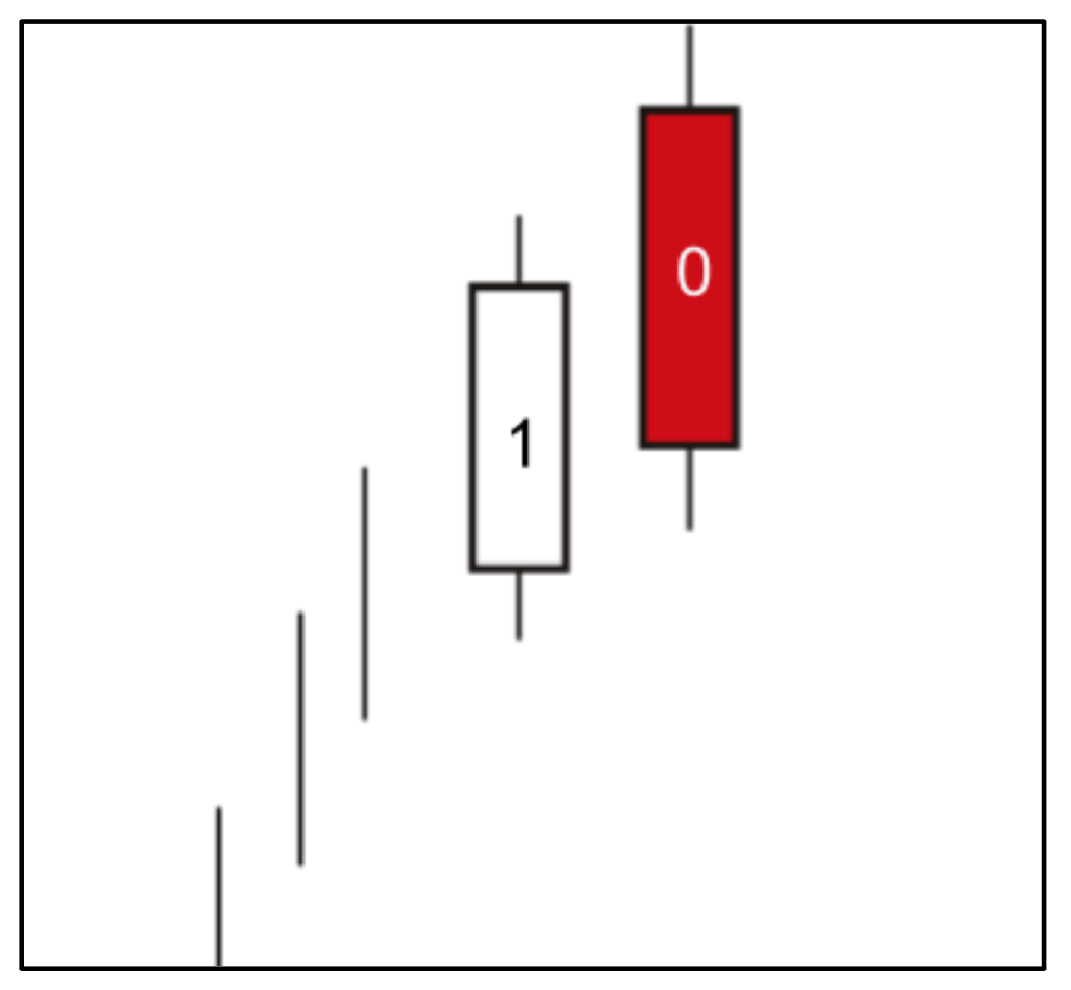
\includegraphics[width=0.5\textwidth]{figuras/f12}
\caption{DarkCloud}
\end{figure}

A Tabela 1  apresenta o tempo gasto para implementar cada algoritmo nas linguagens eleitas para este TCC.

\begin{table}[h]
	\centering
	\label{t01}
	
	\begin{tabular}{ccc}
		\toprule
		\textbf{Linguagem} & \textbf{Tempo médio}\\
		\midrule
		Python & 2 Horas  \\
		Java + JADE & 2 Horas  \\
		MQL4 & 2 Horas  \\
		\bottomrule
	\end{tabular}

	\caption{Tempo médio de implementação do algoritmo}
\end{table}

O algoritmo foi implementado em Java combinado com JADE em um único comportamento, onde o algoritmo concentrado em uma classe é chamado pelo agente. Na linguagem Mql4, o algoritmo implementado retorna uma sinalização visual no gráfico de candlestick, fornecido pela plataforma, alertando a identificação do padrão. Na linguagem Python, o algoritmo implementado retorna uma listagem, contendo informações como datas de ocorrência do padrão, no terminal da IDE utilizada para implementação. Vale ressaltar, que a implementação foi o suficiente para estimar a viabilidade em se implementar a ferramenta proposta no Paradigma de Sistemas Multiagentes.

\item [Analisar Resultado:]
Notou-se que o esforço necessário para implementar o algoritmo nas três linguagens foi aproximadamente o mesmo. Na linguagem Java+JADE e Python, por serem multiplataformas, permitiria desenvolver a ferramenta de forma que a mesma tenha o mesmo comportamento nas plataformas mais populares existentes hoje.

Na ferramenta desenvolvida, um critério de qualidade que merece atenção é a extensibilidade, visando futuras manutenções evolutivas bem como possibilitando trabalhar em mais de um contexto financeiro, como por exemplo, abordar o Mercado de Ações e o Mercado de Renda Fixa simultaneamente. Nesse caso, seria possível trabalhar em um contexto de alto risco de investimento juntamente com um de baixo risco de investimento, obtendo uma melhor gestão de recursos investidos pelo usuário.

Em relação à extensibilidade no contexto financeiro, o Paradigma de Sistemas Multiagentes adequa-se ao estudo, visto que já existe um suporte tecnológico apropriado, um \textit{framework} que atende às necessidades deste TCC. Esse framework oferece um suporte para troca de mensagens entre entidades inteligentes, no contexto abordado neste TCC, entre investidores. Tal suporte baseia-se na comunicação usando protocolos, padrões bem estabelecidos na comunidade de Software para Sistemas Multiagentes e possibilidades de extensibilidade orientadas, por exemplo, a ontologias específicas.

Outro ponto considerado foi que o esforço em se implementar a prova de conceito utilizando a combinação tecnológica linguagem Java e plataforma JADE foi aproximadamente o mesmo em relação às implementações em Python ou Mql4. Portanto, pode-se concluir que a hipótese inicial não se verificou. Assim, a aplicação do Paradigma de Sistemas Multiagentes no contexto financeiro abordado é possível, compreendendo um esforço por parte do desenvolvedor muito próximo aos exigidos nas demais linguagens analisadas.

Finalmente, diante das propriedades do Paradigma de Sistemas Multiagentes, expostas no \textbf{capítulo 2} e a descrição do contexto financeiro exposta no mesmo capítulo, nota-se que existem características comuns entre eles. Nesse cenário, merecem menção as seguintes características:

\begin{enumerate}
\item Autonomia - não há intervenções no processo de decisão de um agente, ele toma decisões sem intervenção de outros agentes ou humanos. Da mesma maneira, um investidor humano também possui autonomia para decidir quando realizar investimentos;

\item Sociabilidade - um agente interage com outros agentes, Software ou humano, através de  algum tipo de linguagem de comunicação. Da mesma maneira, um investidor humano interage com outros atores presentes em uma bolsa de valores, seja para montar grupos, e de maneira conjunta resolver problemas que estão além das suas habilidades individuais, ou apenas para usar serviços disponibilizados por outros atores;

\item Reatividade - um agente fica situado em um ambiente e é capaz de perceber esse ambiente através de seus sensores, é capaz de responder em tempo hábil às mudanças que ocorrem nele. Da mesma maneira, um investidor percebe o ambiente de bolsa de valores no qual está inserido, através de acompanhamentos frequentes de informações que alimentam suas estratégias, e responde às mudanças ocorridas na bolsa de valores de acordo com as informações de saída de suas estratégias;
\item Assincronismo -  um agente, ao receber uma requisição, tem o poder de decidir se irá ou não atender à mesma. Adicionalmente, este agente pode enviar uma requisição a outro agente e continuar suas atividades. Caso não seja atendido, ele tem o poder de enviar a mesma requisição a outros agentes, por exemplo, contornando o problema. Da mesma maneira, um investidor humano pode procurar um ou vários atores presentes na bolsa e escolher aquele que melhor o atende.

\end{enumerate}

Tal fato motivou a exploração do paradigma orientado a agentes no contexto financeiro abordado, cujo objetivo é contribuir com o contexto financeiro através da construção de uma ferramenta de estratégia financeira apoiada por Sistemas Multiagentes Comportamentais, onde não é exigido do usuário conhecimentos relacionados ao Mercado Financeiro. Assim, a ferramenta desenvolvida abstrai a complexidade de cálculos financeiros comumente utilizados na análise técnica e delega ao usuário somente a decisão de comprar ou vender.

\end{description}

\section{Metodologia Adotada no Desenvolvimento da Ferramenta}

A ferramenta resultante deste TCC teve seu desenvolvimento orientando-se de acordo com um modelo de desenvolvimento iterativo e incremental. Para isso, foi escolhida a metodologia ágil  Scrum e foi feita uma adaptação desta, figura 16. As estórias de usuários foram divididas em duas categorias: (i) Produto, são as funcionalidades da ferramenta proposta; e (ii) Pesquisa, são pesquisas realizadas durante as atividades de Engenharia de Software Experimental, principalmente, em relação às provas de conceito. A Tabela 2 apresenta o Product Backlog inicial deste estudo. Vale ressaltar que ele foi modificado durante o desenvolvimento, como previsto no Scrum.

\begin{figure}[h]
\centering
\label{f16}
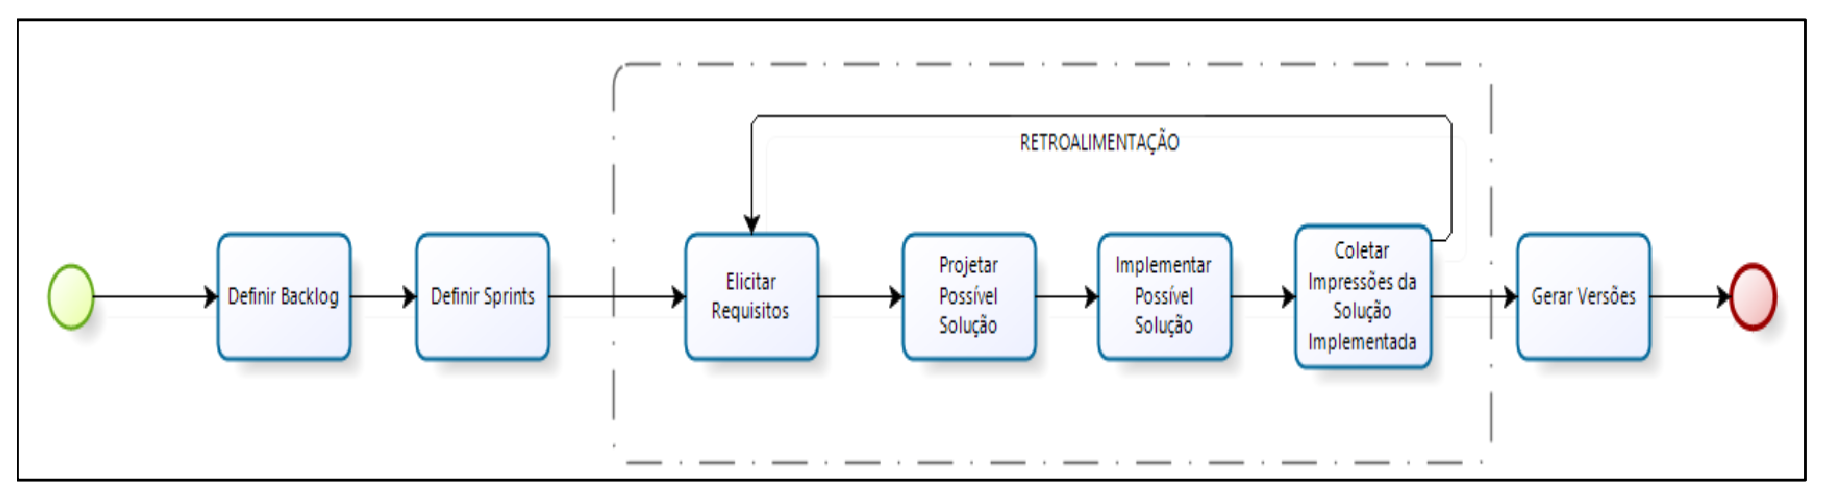
\includegraphics[width=0.9\textwidth]{figuras/f28}
\caption{Scrum adaptado para o TCC}
\end{figure}

\begin{center}
\begin{longtable}{| p{2cm} | p{10cm} |p{3cm} |}
\caption{ProductBacklog inicial} \\
\hline
\textbf{Número} & \textbf{Descrição} & \textbf{Tipo}\\\hline
\endfirsthead
\multicolumn{2}{c}%
{\tablename\ \thetable\ -- \textit{Continuação da página anterior}} \\
\hline
\textbf{Número} & \textbf{Descrição} & \textbf{Tipo}\\\hline
\endhead
\hline \multicolumn{2}{c}{\textit{Continuaçao na próxima página}} \\
\endfoot
\hline
\endlastfoot

	01 & Como engenheiro, quero um agente capaz de montar e gerir uma carteira de ações de acordo com o perfil de investidor escolhido pelo usuário. & Produto\\ \hline
	02 & Como engenheiro, quero um agente capaz de tomar estratégias financeiras de acordo com o perfil de investidor escolhido pelo usuário e valor investido. & Produto\\ \hline
	03 & Como engenheiro, quero um agente capaz de realizar simulações de suas estratégias financeiras no período em que a Bolsa de Valores de São Paulo está fechada. & Produto\\ \hline
	04 & Como engenheiro, quero um agente capaz de realizar buscas contínuas de ações de empresas com presença na Bolsa de Valores de São Paulo e as categorize de acordo com seu setor e retorno diário. & Produto\\ \hline
	05 & Como engenheiro, quero um mecanismo no qual o usuário possa se cadastrar e se vincular a um grupo de agentes. & Produto\\ \hline
	06 & Como engenheiro, quero um código em Python capaz de reconhecer o padrão de \textit{candlestick DarkCloud}, independentemente do ativo analisado para construir estratégias de investimentos mais eficientes. & Pesquisa\\ \hline
	07 & Como engenheiro, desejo definir estratégias de investimentos para servir de apoio aos agentes.. & Pesquisa\\ \hline
	08 & Como engenheiro, quero um código em MQL4 capaz de reconhecer o padrão de \textit{candlestick DarkCloud}, independentemente do ativo analisado para construir estratégias de investimentos mais eficientes . & Pesquisa\\ \hline
	09 & Como engenheiro, quero um código em Java+JADE capaz de reconhecer o padrão de \textit{candlestick DarkCloud}, independentemente do ativo analisado para construir estratégias de investimentos mais eficientes. & Pesquisa

\label{t05}
\end{longtable}
\end{center}


Nas estórias do tipo Produto, foram criadas tarefas que nortearam a implementação das estórias iniciais. Estas foram distribuídas em Sprints de 4 semanas bem como intercaladas com atividades de documentação de TCC. A listagem a seguir apresenta as tarefas por estória de usuário: 

\begin{enumerate}
\item Eu como engenheiro, quero um agente capaz de montar e gerir uma carteira de ações de acordo com o perfil de investidor escolhido pelo usuário.
		\begin{itemize}
		\item Implementar comunicação entre agentes gestores e caçadores;
		\item Implementar comunicação entre agentes gestores e especialistas;
		\item Implementar rotina de cálculo de riscos de carteiras para agentes gestores;
		\item Implementar critério de intervenção em operações que representem risco em desacordo com o perfil escolhido pelo usuário;
		\item Implementar rotina de criação e destruição de agentes especialistas;
		\item Implementar rotina de montagem de carteira de ações;
		\item Implementar rotina de autorização de operações.
		\end{itemize}
\item Eu como engenheiro, quero um agente capaz de tomar estratégias financeiras de acordo com o perfil de investidor escolhido pelo usuário e valor investido.
		\begin{itemize}
		\item Implementar rotinas de acompanhamento de ações de empresas que compõem a carteira de investimentos;
		\item Implementar rotinas de solicitação de autorização de operações.
		\item Implementar estratégia financeira baseada em Médias Móveis;
		\item Implementar estratégia financeira baseada em Padrões de Candlesticks; 
		\end{itemize}
\item Eu como engenheiro, quero um agente capaz de realizar simulações de suas estratégias financeiras no período em que a Bolsa de Valores de São Paulo está fechada;
		\begin{itemize}
		\item Implementar rotina de simulação de estratégias em dados históricos;
		\item Implementar rotina de persistência de resultados obtidos.
		\end{itemize}

\item Eu como engenheiro, quero um agente capaz de realizar buscas contínuas de ações de empresas com presença na Bolsa de Valores de São Paulo e as categorizar de acordo com seu setor e retorno diário.
		\begin{itemize}
		\item Implementar rotinas de busca de ações na Bolsa de Valores de São Paulo;
		\item Implementar rotinas de triagem e persistência de ações;
		\item Implementar rotinas de criação de agentes caçadores.
		\end{itemize}

\item Eu como engenheiro, quero um mecanismo, no qual o usuário possa se cadastrar e se vincular a um grupo de agentes.
		\begin{itemize}
		\item Implementar interface com o usuário e rotina de login;
		\item Implementar rotina de instanciação de agentes gestores.
		\end{itemize}

\end{enumerate}

Como previsto na metodologia Ágil Scrum, durante o desenvolvimento da ferramenta foi necessário modificar o Backlog inical. Dentre estas modificações temos : (i) a divisão da estória 01 em duas; (ii) a remoção da estória 03; e (iii) a criação de uma estória relacionada à comunicação dos usuários com seus respectivos agentes.

Quanto à estória 01 - "Eu como engenheiro, quero um agente capaz de montar e gerir uma carteira de ações de acordo com o perfil de investidor escolhido pelo usuário e valor investido.". Esta foi dividida nas seguintes estórias com suas respectivas tarefas:

\begin{description}
\item[Estória 01:]
Eu como engenheiro, quero um agente capaz de montar uma carteira de ações de acordo com o perfil escolhido pelo usuário.

\begin{itemize}
		\item Implementar comunicação entre agentes gestores e caçadores;
		\item Implementar comunicação entre agentes gestores e especialistas;
		\item Implementar rotina de montagem de carteira de ações;
		

\end{itemize}

\item[Estória 10:]
Eu como engenheiro, quero um agente capaz de gerir uma carteira de ações de acordo com o perfil escolhido pelo usuário.
\begin{itemize}

	\item Implementar rotina de cálculo de riscos de carteiras para agentes gestores;
	\item Implementar critério de intervenção em operações que representem risco em desacordo com o perfil escolhido pelo usuário;
	\item Implementar rotina de criação e destruição de agentes especialistas;
	\item Implementar rotina de autorização de operações.

\end{itemize}
\end{description}

Quanto à estória 03 - "Como engenheiro, quero um agente capaz de realizar simulações de suas estratégias financeiras no período em que a bolsa de valores de São Paulo está fechada.". Esta foi removida do Backlog. Durante o desenvolvimento da ferramenta, verificou-se que a implementação desta estória comprometeria a entrega final. Tal aspecto foi verificado, uma vez que esta estória demanda a criação de uma máquina de aprendizado baseada em inteligência artificial de modo a aproveitar ao máximo os dados obtidos com simulações automáticas. Esta máquina de aprendizado é uma forte candidata à uma futura manutenção evolutiva.

Quanto à estória 11 - "Como engenheiro, quero um agente capaz de prover a comunicação entre os usuários e seus respectivos agentes.". Esta foi criada durante o desenvolvimento da ferramenta, onde verificou-se a necessidade de criar um agente responsável por monitorar novos cadastros de usuários e, assim, criar e vincular um agente. Adicionalmente, verificou-se a necessidade de monitorar ações de \textit{log in} dos usuários. O agente implementado nesta estória é apresentado como Agente Criador no capítulo 5. As tarefas relacionadas a essa estória são apresentadas a seguir.

\begin{description}
\item[Estória 11:]
Como engenheiro, quero um agente capaz de prover a comunicação entre os usuários e seus respectivos agentes.

\begin{itemize}

\item Implementar comportamento de monitoramento de criação de novos usuários;
\item Implementar comportamento de monitoramento de \textit{log in} de usuários;
\item Implementar rotina de criação de agentes gestores;
\item Implementar comunicação entre agentes criadores e gestores;

\end{itemize}

\end{description}

A tabela 3 apresenta o cronograma seguido no desenvolvimento das estórias de usuário, vale ressaltar que as atividades executadas nos meses de abril e maio de 2015 são relacionadas à atividade "Coletar Impressões da ferramenta", descrita brevemente na subsessão 4.3. As tabelas 4, 5 e 6 apresentam  o Backlog final da ferramenta, bem como os percentuais de conclusão das tarefas por estórias e da ferramenta de maneira geral.

\begin{center}
\begin{longtable}{| p{2cm} | p{5cm} |p{3cm} |p{2cm} |}
\caption{Cronograma} \\
\hline
\textbf{Sprint} & \textbf{Atividade} & \textbf{Data início} & \textbf{Data fim}\\ \hline
\endfirsthead
\multicolumn{2}{c}%
{\tablename\ \thetable\ -- \textit{Continuação da página anterior}} \\
\hline
\textbf{Sprint} & \textbf{Atividade} & \textbf{Data início} & \textbf{Data fim}\\ \hline
\endhead
\hline \multicolumn{2}{c}{\textit{Continuaçao na próxima página}} \\
\endfoot
\hline
\endlastfoot

{Sprint 1} & Implementar estórias 06/07/08/09   &03/03/14 &28/03/14 \\ \hline
{Sprint 2} & Implementar estória 05 &04/08/14 &29/08/14 \\ \hline
{Sprint 3} & Implementar estória 11 &01/09/14 &26/09/14 \\ \hline
{Sprint 4} & Implementar estória 01 &01/10/14 &30/10/14 \\ \hline
{Sprint 5} & Implementar estória 02 &03/11/14 &28/11/14 \\ \hline
{Sprint 6} & Implementar estória 04 &01/12/14 &12/12/14 \\ \hline
{Sprint 7} & Implementar estória 10 &02/03/15 &27/03/15 \\ \hline
{Sprint 8} & Coleta de impressões &01/04/14 &30/04/15 \\ \hline
{Sprint 9} & Coleta de impressões &04/05/14 &29/04/15  

\label{t03}
\end{longtable}
\end{center}



\begin{center}
\begin{longtable}{| p{2cm} | p{8cm} |p{2cm} |}
\caption{Backlog final: estórias de produto concluídas} \\
\hline
\textbf{Estória} & \textbf{Tarefa} & \textbf{Percentual}\\ \hline
\endfirsthead
\multicolumn{2}{c}%
{\tablename\ \thetable\ -- \textit{Continuação da página anterior}} \\
\hline
\textbf{Estória} & \textbf{Tarefa} & \textbf{Percentual}\\ \hline
\endhead
\hline \multicolumn{2}{c}{\textit{Continuaçao na próxima página}} \\
\endfoot
\hline
\endlastfoot

	{} & Implementar comunicação entre agentes gestores e caçadores; & 100\% \\ \cline{2-3}
	01 & Implementar comunicação entre agentes gestores e especialistas; & 100\% \\ \cline{2-3}
	{} & Implementar rotina de montagem de carteira de ações; & 100\% \\  \hline
	
	{} & Implementar rotinas de acompanhamento de ações de empresas que compõem a carteira de investimentos; & 100\% \\ \cline{2-3}
	{} & Implementar rotinas de solicitação de autorização de operações; & 100\% \\ \cline{2-3}
	02 & Implementar estratégia financeira baseada em Médias Móveis; & 100\% \\ \cline{2-3}
	{} & Implementar estratégia financeira Padrões de Candlesticks; & 100\% \\ \hline


	{} & Implementar rotinas de busca de ações na Bolsa de Valores São Paulo; & 100\% \\ \cline{2-3}
	04 & Implementar rotinas de triagem e persistência de ações; & 100\% \\ \cline{2-3}
	{} & Implementar rotinas de criação de agentes caçadores; & 100\% \\ \hline

	05 & Implementar interface com o usuário e rotina de login; & 100\% \\ \cline{2-3}
	{} & Implementar rotina de instanciação de agentes gestores; & 100\% \\ \hline

	{} & Implementar rotina de cálculo de riscos de carteiras para agentes gestores; & 100\% \\ \cline{2-3}
	10 & Implementar critério de intervenção em operações que representem risco em desacordo com o perfil escolhido pelo usuário; & 100\% \\ \cline{2-3}
	& Implementar rotina de criação e destruição de agentes especialistas; & 100\% \\ \cline{2-3}
	{} & Implementar rotina de autorização de operações. ; & 100\% \\ \hline

	{} & Implementar comportamento de monitoramento de criação de novos usuários; & 100\% \\ \cline{2-3}
	11 & Implementar comportamento de monitoramento de \textit{log in} de usuários; & 100\% \\ \cline{2-3}
	{} & Implementar comunicação entre agentes criadores e gestores; & 100\% \\ \cline{2-3}
	{} & Implementar rotina de criação de agentes gestores; & 100\% \\ \hline

	{} & Total & 100,00\% 
	
\label{t04}
\end{longtable}
\end{center}


\begin{center}
\begin{longtable}{| p{2cm} | p{8cm} | p{2cm} |}
\caption{Percentual de estórias de pesquisas concluídas} \\
\hline
\textbf{Número} & \textbf{Descrição}  & \textbf{Percentual}\\ \hline
\endfirsthead
\multicolumn{2}{c}%
{
\tablename\ \thetable\ -- \textit{Continuação da página anterior}} \\
\hline
\textbf{Número} & \textbf{Descrição}  & \textbf{Percentual}\\ \hline
\endhead
\hline \multicolumn{2}{c}{\textit{Continuaçao na próxima página}} \\
\endfoot
\hline
\endlastfoot
	06 & Eu, como pesquisador, quero um código em Python capaz de reconhecer o Padrão de Candlestick DarkCloud, independentemente do ativo analisado para construir estratégias de investimentos mais eficientes & 100\% \\ \hline
	07 & Eu, como pesquisador, desejo definir estratégias de investimentos de curto prazo em um agente visando testar sua capacidade em atuar no mercado; & 100\%\\ \hline
	08 & Eu, como pesquisador, quero um código em MQL4 capaz de reconhecer o Padrão de Candlestick DarkCloud, independentemente do ativo analisado para construir estratégias de investimentos mais eficientes; & 100\%\\ \hline
	09 & Eu, como pesquisador, quero um código em Java+ JADE capaz de reconhecer o Padrão de Candlestick DarkCloud, independentemente do ativo analisado para construir estratégias de investimentos mais eficientes. & 100\%\\ \hline
	{} & Total Concluído. & 100\%
\label{t05}
\end{longtable}
\end{center}


\begin{center}
\begin{longtable}{| p{5cm} | p{6cm} |p{5cm} |}
\caption{Percentual geral de conclusão da ferramenta} \\
\hline
\textbf{Item} & \textbf{Percentual do item}  & \textbf{Percentual relativo}\\ \hline
\endfirsthead
\multicolumn{2}{c}%
{\tablename\ \thetable\ -- \textit{Continuação da página anterior}} \\
\hline
\textbf{Item} & \textbf{Percentual do item}  & \textbf{Percentual Relativo}\\ \hline
\endhead
\hline \multicolumn{2}{c}{\textit{Continuaçao na próxima página}} \\
\endfoot
\hline
\endlastfoot
	Estória de Produto & 100\% .& 100\% de 84\%\\ \hline
	Estória de Pesquisa & 100\% & 100\% de 16\%.\\\hline
	{} & Total geral & 100\%
\label{t06}
\end{longtable}
\end{center}



\section{Metodologia Adotada na Análise dos Resultados Obtidos}


O resultado obtido neste TCC foi avaliado de maneira quantitativa e qualitativa. 

Quantitativa através da cobertura de código e métricas de qualidade de código, tais como : (i) Complexidade Ciclomática - CC, adotado para auxiliar no controle dos possíveis caminhos dos algoritmos; (ii)  Coesão e Acoplamento  - SC, adotado para mensurar o grau de reusabilidade dos pacotes projetados; e (iii) Herança - DIT, adotado para mensurar o grau de encapsulamento. Qualitativa através de questionários aplicados em potenciais usuários da ferramenta com intuito de mensurar o grau de aceitação do usuário, bem como verificar os objetivos adotados neste TCC. Outros dados quanto aos resultados obtidos são apresentados detalhadamente no capitulo 6.


\section{Resumo do Capítulo}

Elucidou-se neste capítulo, um breve levantamento acerca das principais metodologias de pesquisa científica encontradas na literatura, tais como: (i) pesquisa descritiva; (ii) pesquisa explicativa; e (iii) pesquisa exploratória. Esta última sendo a que mais se adequou ao tema coberto neste Trabalho de Conclusão de Curso. 

Foi descrita ainda, a metodologia utilizada para condução do Trabalho de Conclusão de Curso como um todo. Adicionalmente, foram descritas as metodologias que conduziram o desenvolvimento da ferramenta em si e a análise dos resultados obtidos.

Na subseção 4.3, foram descritas as atividades que compõem a metodologia utilizada para condução do Trabalho de Conclusão de Curso como um todo. Dentre as atividades descritas, destacou-se a atividade de desenvolvimento de provas de conceito, a qual foi de suma importância para definir o suporte tecnológico adequado ao desenvolvimento da ferramenta.   

Na subseção 4.4, foi apresentada a metodologia que conduziu o desenvolvimento da ferramenta em si. No caso, optou-se por uma adaptação da metodologia ágil Scrum. Foi apresentado ainda nesta subseção, o Product Backlog inicial da ferramenta bem como suas modificações e distribuição no cronograma.

Por fim, na subseção 4.5, foi apresentada a metodologia que orientou a análise dos resultados obtidos. No caso, optou-se por avaliálos de forma quantitativa, através da cobertura de código e de métricas de qualidade de código. Adicionalmente, optou-se por avaliá-los de forma qualitativa, através de questionários aplicados junto aos pontenciais usuários da ferramenta.


\newpage
\chapter[FERRAMENTA FINANCEIRA]{Ferramenta Financeira}

Esse capítulo apresenta em detalhes a ferramenta desenvolvida para o contexto do Mercado Financeiro de Bolsa de Valores usando uma abordagem Multiagentes. O capítulo está organizado em seções. Na primeira seção, serão detalhados os diferentes níveis arquiteturais que compõem a estrutura geral da ferramenta. Salienta-se que o primeiro nível arquitetural corresponde à arquitetura base, a qual orientou a comunicação dos agentes, o ciclo de vida dos mesmos, protocolos de interação, suas criações, registros de serviços prestados e outros detalhes inerentes à programação multiagentes. A arquitetura base utilizada é a da Plataforma JADE. Essa foi apresentada no capítulo de Suporte Tecnológico, seção 3.2.3. Em um segundo momento, será apresentada a arquitetura da ferramenta em si, a qual foi organizada de acordo com o padrão arquitetural Model-View-Controller (MVC). Adicionalmente, será apresentada a arquitetura da máquina de raciocínio dos agentes, onde cada agente será descrito em detalhes bem como suas estratégias de ação no contexto financeiro. Esse último nível arquitetural foi quem mais demandou esforços nesse Trabalho de Conclusão de Curso, por representar a lógica de raciocínio dos agentes, e, portanto, o core da ferramenta. Por fim, é acordada uma abordagem evolutiva, visando facilitar a manutenção bem como a refatoração da ferramenta.

\section{Níveis Arquiteturais da Ferramenta}
A ferramenta compreende três níveis arquiteturais, sendo cada um deles brevemente descrito a seguir:

\begin{description}
\item[Primeiro Nível Arquitetural:]
esse primeiro nível arquitetural corresponde à arquitetura base. Nesse escopo, a ferramenta está orientada pela arquitetura da própria plataforma JADE. Essa arquitetura provê recursos, padronizados pela Foundation for Intelligent Physical Agents (FIPA) \cite{telecon2014}, visando facilitar, dentre outras ações da programação multiagentes: (i) ciclo de vida dos agentes, orientado de acordo com uma máquina de estados desenhada especificamente para sistemas multiagentes comportamentais; (ii) comunicação entre os agentes, garantindo que a interação entre os agentes seja realizada via protocolos e ontologias pré-estabelecidos; (iii) registro dos serviços prestados pelos agentes, facilitando a busca por serviços bem como a localização de um agente em específico; (iv) criação dos agentes, (v) transporte de mensagens, com acompanhamento de troca de mensagens em tempo real, via ferramentas gráficas, e (vi) especificação dos comportamentos, orientando-se pelos tipos de comportamentos estabelecidos na plataforma, sejam eles simples ou compostos.

\item[Segundo Nível Arquitetural:]
esse segundo nível arquitetural corresponde à arquitetura da ferramenta em si, a qual se orienta pelo padrão arquitetural MVC. Esse padrão foi utilizado, pois a ferramenta é disponibilizada via Web. Dessa forma, a estrutura de pacotes da ferramenta está organizada em três camadas: modelo, visão e controle. Detalhes desse nível arquitetural são acordados nesse capítulo, mais especificamente na próxima seção.

\item[Terceiro Nível Arquitetural:]
esse nível arquitetural corresponde à arquitetura da máquina de raciocínio dos agentes. Essa pode ser vista como o core da ferramenta, pois seu escopo corresponde à lógica dos agentes. Essa lógica implementa o \textit{rationale} dos agentes, ou seja, como eles raciocinam e quais ações desempenham. Esse nível arquitetural foi o que demandou maior dedicação ao longo do trabalho aqui apresentado. Visando facilitar o entendimento, a máquina de raciocínio dos agentes pode ser entendida como fazendo parte da camada de controle, quando associada ao modelo MVC. Esse nível arquitetural também é detalhado nesse capítulo, na seção 5.3.

\end{description}

\section{Arquitetura da Ferramenta}

Existem duas características que norteiam o desenvolvimento de um Software na atualidade, manutenabilidade e reusabilidade. Para viabilizar que a ferramenta desenvolvida neste TCC atenda essa visão de desenvolvimento de Software, manutenível bem como reutilizável, aliado ao fato da ferramenta ser Web, o modelo arquitetural escolhido foi o MVC \cite{krasner1988}. Dessa forma, os códigos implementados no Paradigma de Sistemas Multiagentes possuem um alto grau de modularização, baixo acoplamento e alta coesão. Assim, a ferramenta desenvolvida possibilita a realização de  manutenções de maneira mais eficiente, dado que o contexto financeiro compreende regras de negócio de alta mutabilidade. 

Em View ou Visão , figura 17 , concentram-se todos os códigos relacionados à interface com o usuário, esta construída através do Grails versão 2.4.3. Em Controller ou Controle, figura 18, concentraram-se os códigos responsáveis por conectar o usuário com os agentes implementados, representando a máquina de raciocínio dos agentes - o \textit{core} central do Sistema Multiagentes. Em Model ou Modelo, figura 18, concentram-se as entidades do modelo de domínio, representando os agentes de Software, outros modelos conceituais pertinentes (ex. protocolos de comunicação utilizados, regras de negócio do contexto financeiro e outros) e modelo de entidades da camada de persistência.

\begin{figure}[h]
\centering
\label{f17}
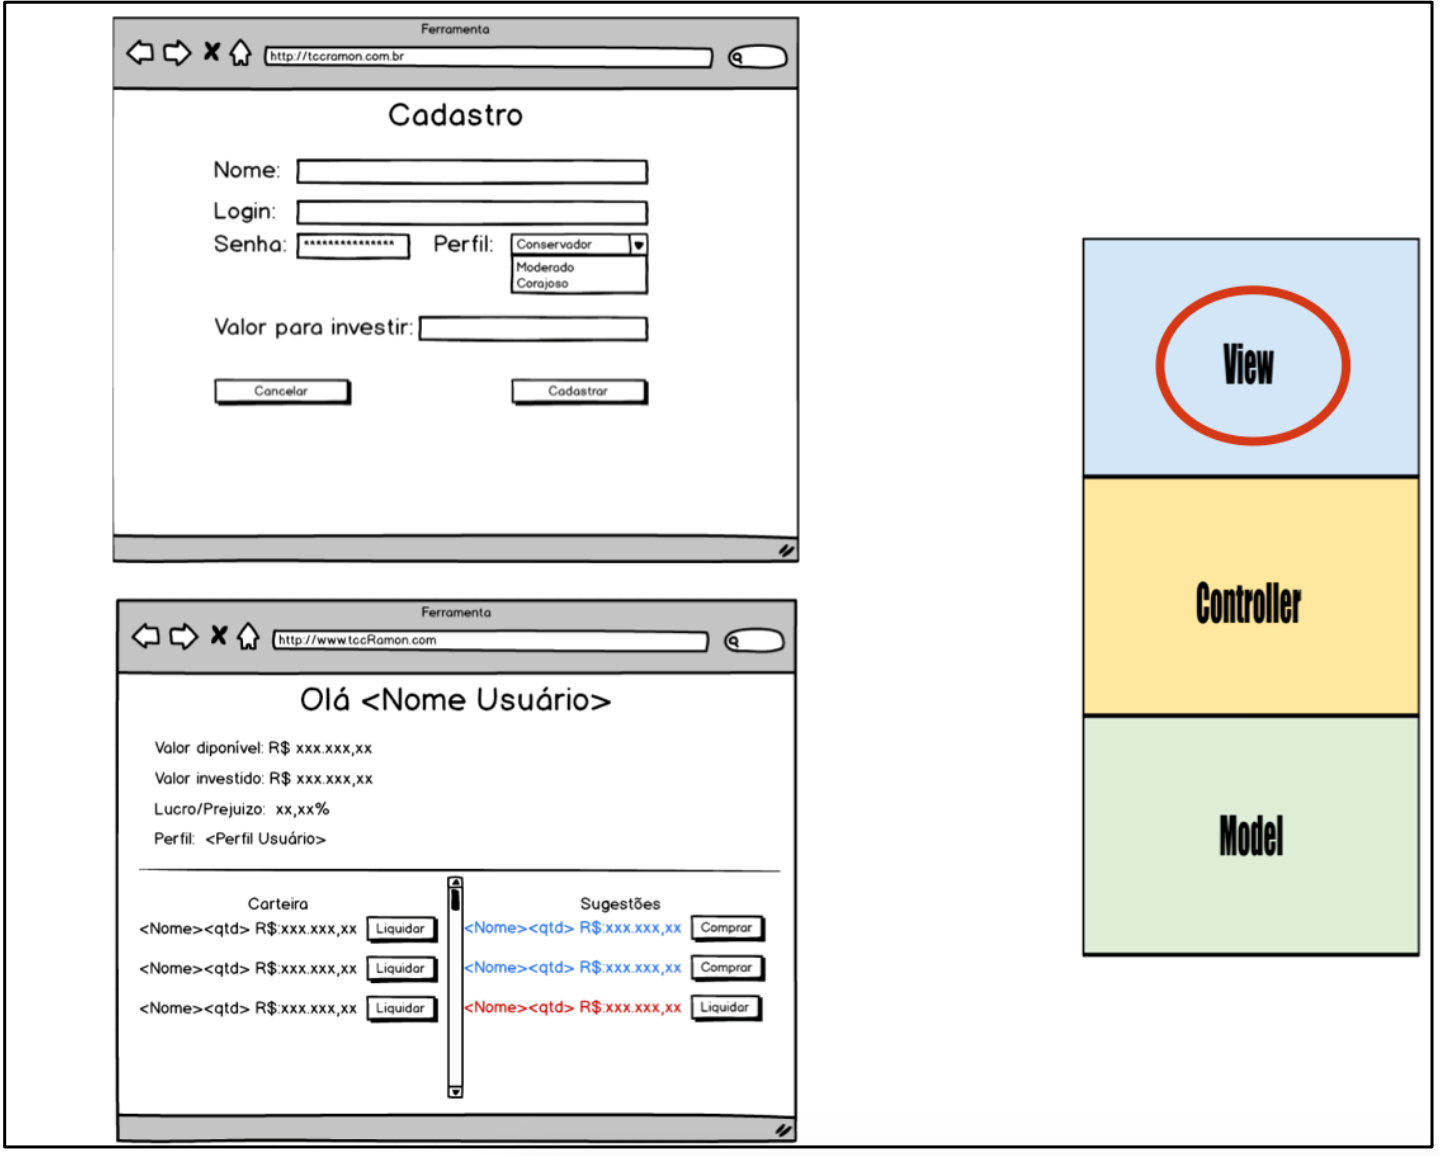
\includegraphics[width=0.9\textwidth]{figuras/f24}
\caption{Camada View}
\end{figure}

\begin{figure}[h]
\centering
\label{f18}
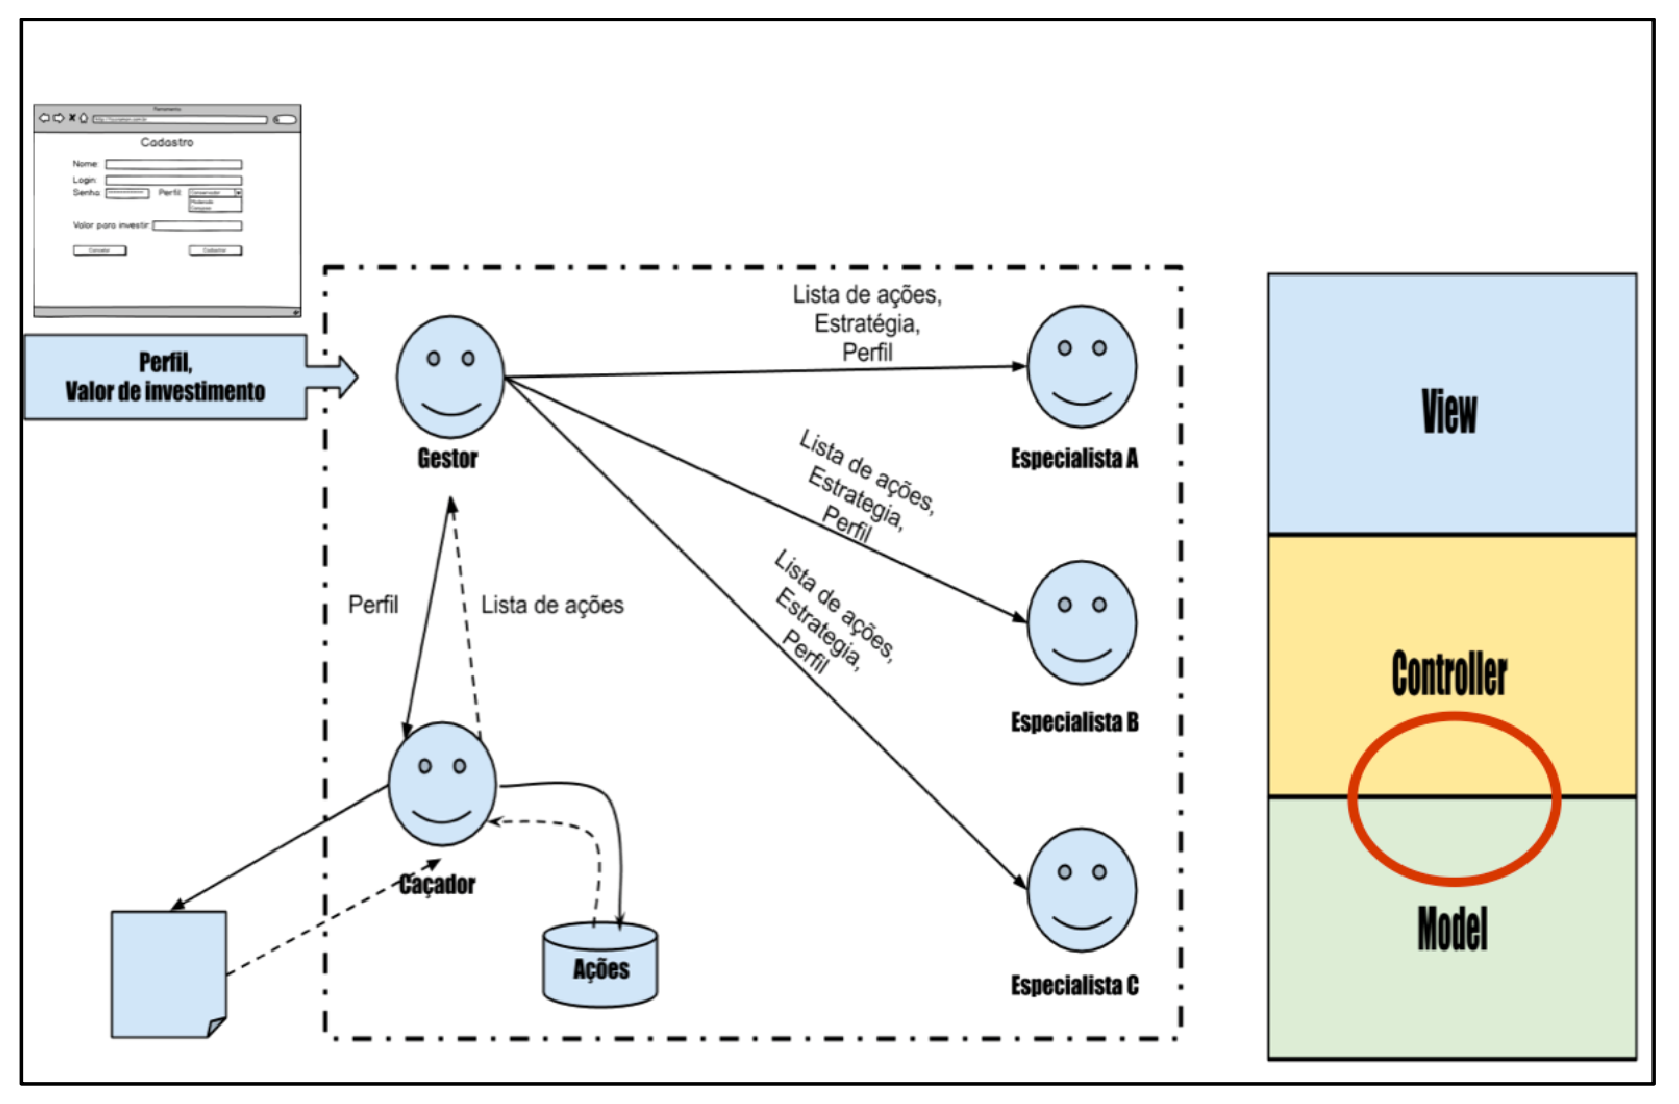
\includegraphics[width=0.9\textwidth]{figuras/f25}
\caption{Controller-Model}
\end{figure}
\FloatBarrier

Vale ressaltar que a Camada de Controle contém o pacote core (figura 19), nele estão concentrados os códigos que implementam os agentes comportamentais e suas classes de suporte. Apresenta-se neste pacote de maneira adicional, uma estrutura proposta para futura refatoração arquitetural da ferramenta (figura 20), no tocante aos comportamentos dos agente.

\begin{figure}[h]
\centering
\label{f19}
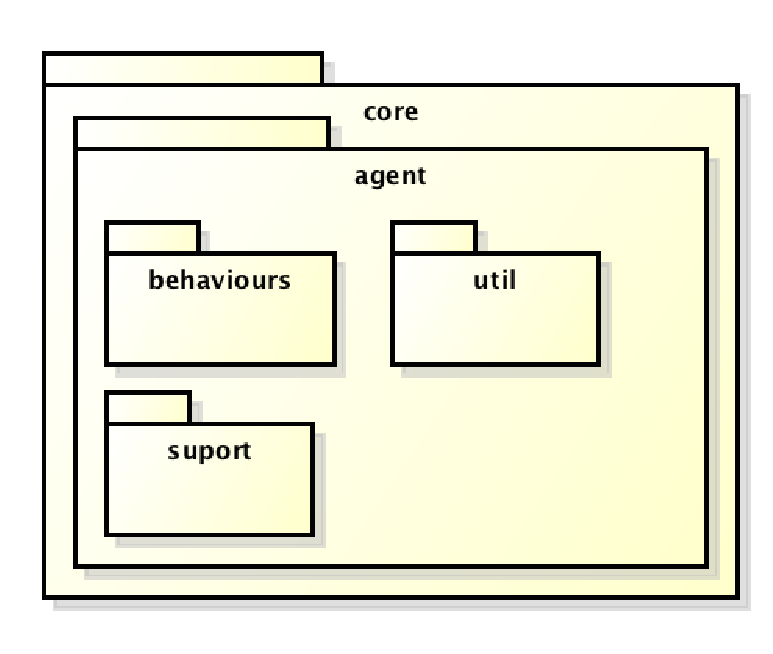
\includegraphics[width=0.6\textwidth]{figuras/pacoteAgents}
\caption{Pacote core}
\end{figure}

\begin{figure}[h]
\centering
\label{f20}
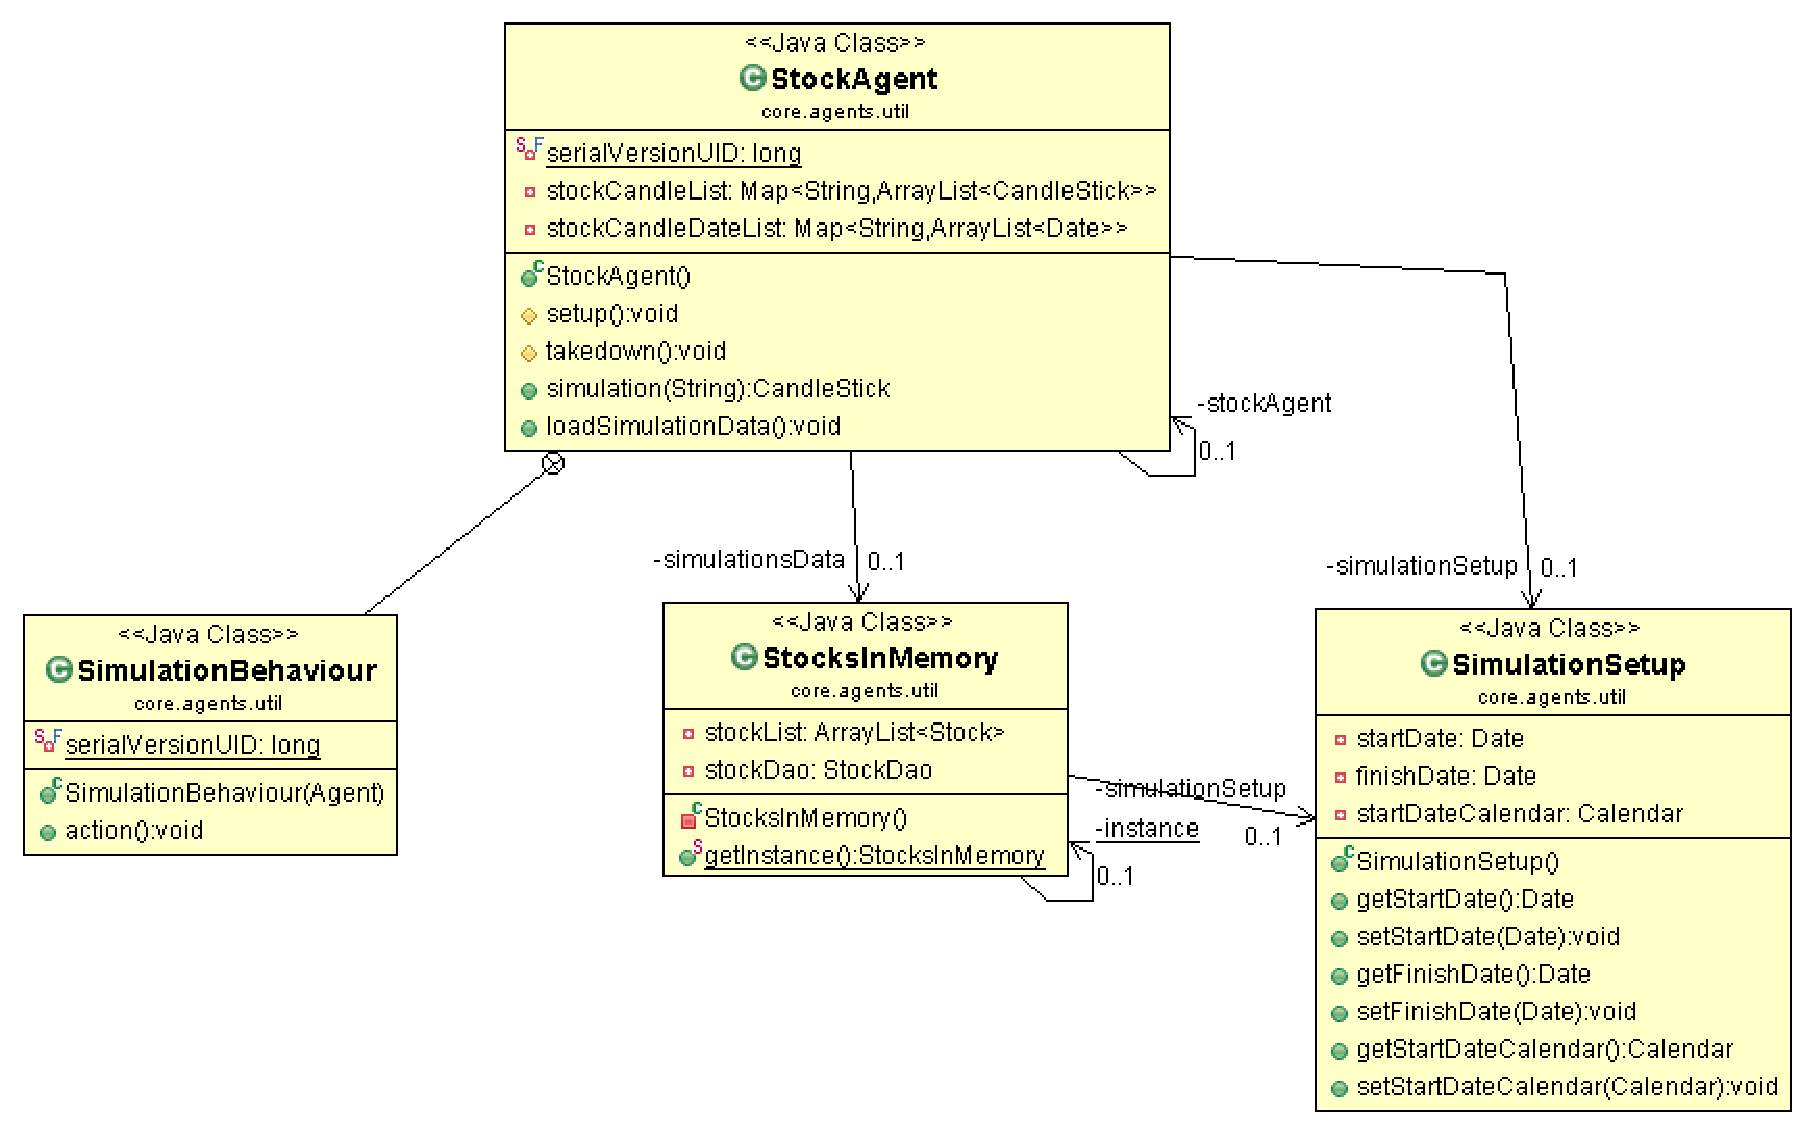
\includegraphics[width=0.8\textwidth]{figuras/classesUtil}
\caption{Estrutura elaborada para execução da Ferramenta em modo offline}
\end{figure}

O Subpacote agent contém os subpacotes: (i) behaviours, comporta classes que implementam comportamentos e estrutura de construção de comportamento proposto pelo autor como refatoração futura; (ii) suport, comporta classes que auxiliam os agentes comportamentais implementados; e (iii) util, comporta classes que compõem a estrutura desenvolvida pelo autor para contornar o problema de ausência de conexão com internet. 

A estrutura desenvolvida para contornar uma possível falha de ausência de conexão com internet é composta por quatro classes (figura 20): (i) StockAgent, classe que implementa um agente responsável por simular as ações do servidor de cotações; (ii) SimulationBehaviour, classe que implementa o comportamento de resposta à uma requisição de cotação; (iii) StocksInMemory, classe utilizada para carregar uma seleção de dados na memória do computador, dados estes que serão enviados aos agentes que solicitarem cotações; e (iv) SimulationSetup, classe que contém dados essenciais para o funcionamento da ferramenta em modo \textit{offline}.

A camada de Modelo comporta classes  essenciais para o funcionamento da ferramenta e dos agentes em si. Estas classes está organizadas no pacote suport (figura 21). O pacote suport contém três subpacotes: (i) financial, contém as classes responsáveis por prover estratégias financeiras a serem utilizadas por agentes especialistas (figura 22); (ii) util, contém classes responsáveis por prover o mecanismo de persistência em banco de dados e responsáveis pela lógica de requisição de dados de cotação de ações; e o subpacote (iii) statistical, contém as classes responsáveis por prover mecanismos de cálculos estatísticos utilizados pelos agentes caçadores, no processo de triagem e ações, e pelos agentes gestores, no processo de controle de risco.   

\begin{figure}[h]
\centering
\label{f21}
\includegraphics[width=0.5\textwidth]{figuras/pacoteSuport}
\caption{Pacote suport}
\end{figure}


\begin{figure}[h]
\centering
\label{f22}
\includegraphics[width=1\textwidth]{figuras/estrategias}
\caption{Estrutura desenvolvida para o uso de estratégias financeiras}
\end{figure}
\FloatBarrier

\section{Arquitetura da Máquina de Raciocínio dos Agentes}

A ferramenta desenvolvida atua considerando três tipos de perfis de investidor, de forma a contribuir na realização do maior lucro possível de acordo com o perfil do usuário, ou seja, sob a perspectiva de investimento cabível para esse usuário. Informações sobre os perfis são simplificadamente providas na Tabela 7.

\begin{center}
\begin{longtable}{| p{8cm} | p{8cm} |}
\caption{Perfis de investidores} \\
\hline
\textbf{Perfil } & \textbf{Descrição} \\ \hline
\endfirsthead
\multicolumn{2}{c}%
{\tablename\ \thetable\ -- \textit{Continuação da página anterior}} \\
\hline
\textbf{Perfil } & \textbf{Descrição} \\ \hline
\endhead
\hline \multicolumn{2}{c}{\textit{Continuaçao na próxima página}} \\
\endfoot
\hline
\endlastfoot
	Corajoso & São pessoas que, dentre os três perfis, assumem o maior risco e estão dispostas a acompanhar com maior frequência a movimentação do Mercado Financeiro.\\ \hline
	Moderado & São pessoas que estão entre os perfis Corajoso e Conservador. Esse perfil adequa-se às pessoas que desejam operar esporadicamente no Mercado Financeiro, mas com um certo nível de risco.\\\hline
	Conservador & São pessoas que desejam gerir seu próprio plano de aposentadoria complementar, utilizando o Mercado Financeiro Brasileiro. Pessoas com este perfil desejam apenas arrecadar um capital suficiente para garantir seu padrão de vida, ou seja, são pessoas que desejam lucros razoáveis com um grau de risco menor do que os demais perfis.
\label{t07}
\end{longtable}
\end{center}
\subsection{Principais agentes}

Foram projetados inicialmente três tipos de agentes comportamentais: (i) agente gestor; (ii) agente especialista, e (iii) agente caçador. No entanto, durante o desenvolvimento da ferramenta verificou-se a necessidade em criar um quarto tipo de agente de Software, o agente criador. Este é responsável por auxiliar na comunicação entre usuários web com seus respectivos agentes de Software, mais internos à lógica da ferramenta. 

\begin{description}
\item[Agente gestor (manager):]
O agente do tipo gestor é o responsável por administrar a carteira de ações dos usuários, ações que por sua vez são acompanhadas por agentes especialistas. Ele autoriza uma compra ou venda de ações analisadas pelos agentes especialistas. Vale ressaltar que essa autorização passa pelo usuário vinculado ao grupo de agentes. O agente gestor, de maneira autônoma, faz o monitoramento de risco envolvido na carteira de ações administrada. Adicionalmente, executa o processo de montagem de carteira de maneira alinhada com o perfil escolhido pelo usuário. Suas responsabilidades são:

\begin{itemize}
\item Criar e excluir um ou mais agentes especialistas:\newline

A quantidade de agentes especialistas criadas pelo agente gestor varia  de acordo com o perfil de usuário. Portanto, podem ser criados: (i) dois agentes especialistas para o perfil Corajoso; (ii) quatro agentes especialistas para o perfil Moderado; e (iii) sete agentes especialistas para o perfil Conservador.

\item Montar carteira de ações:\newline

Após instanciados os agentes para o usuário, o agente gestor verifica qual foi o perfil escolhido pelo usuário em seu cadastro e inicia o processo de montagem de carteira de ações (figura 23). Ele interage com um agente caçador e solicita um número determinado de ações, de acordo com o perfil do usuário. Segundo Pinheiro (\citeyear{pinheiro2008}, p.93), uma carteira com ações de 30 empresas diferentes pode ser considerada como uma carteira conservadora. Com base neste número, foi derivada a quantidade de ações por carteira de cada tipo de perfil. Assim, para o perfil Conservador, a carteira é formada por ações de 30 empresas. Para o perfil Moderado, 13 empresas. Já o perfil Corajoso, 8 empresas. Vale ressaltar que esses números iniciais foram baseados na recomendação do autor Pinheiro (\citeyear{pinheiro2008}, p.93), combinados com os números da sequência de Fibonacci. Essa sequência é bastante aceita no meio financeiro. Adicionalmente, esses valores iniciais poderão ser melhorados em futuras versões da ferramenta, caso seja necessário.

\begin{figure}[H]
\centering
\label{f23}
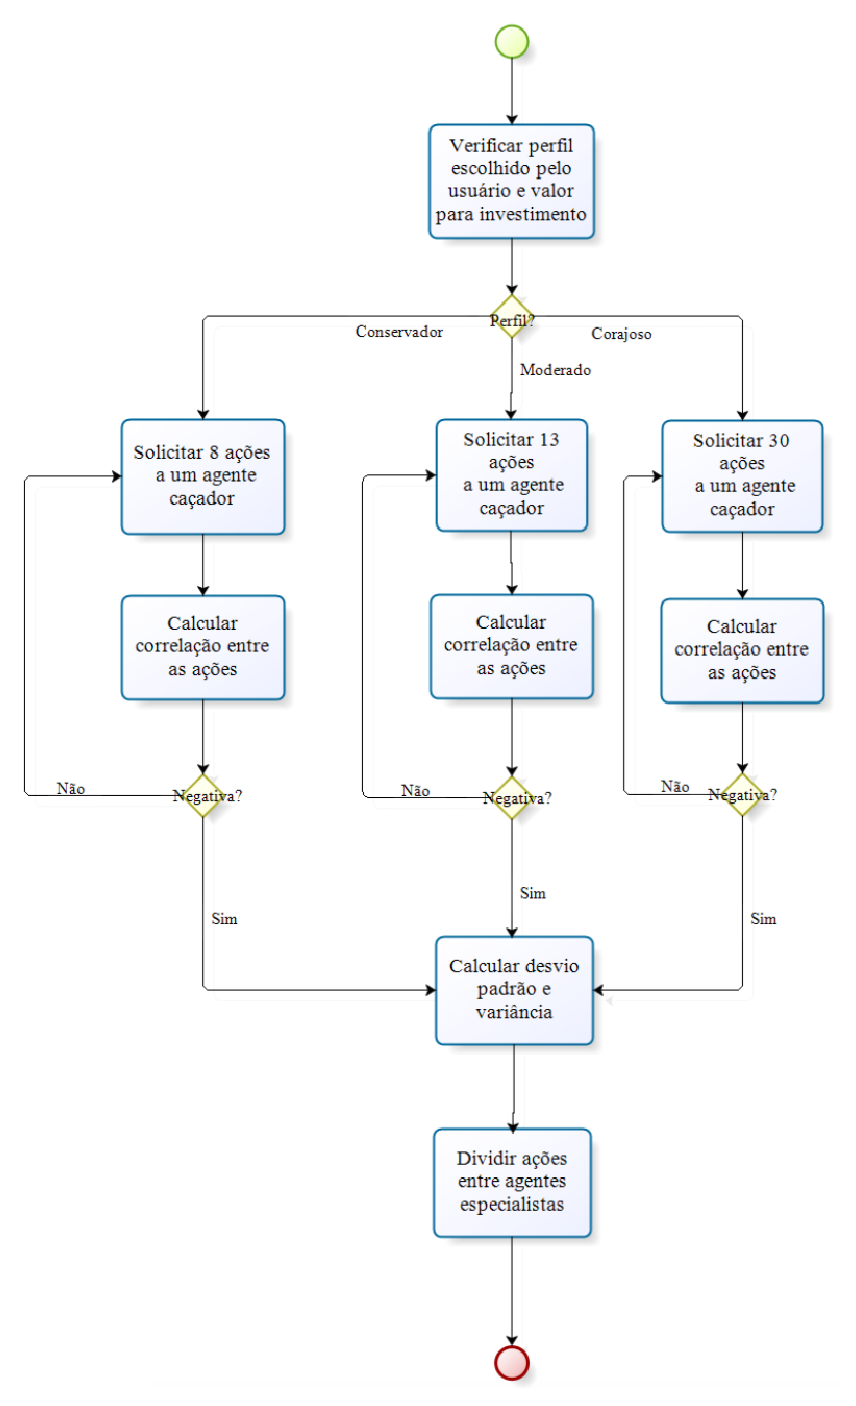
\includegraphics[width=0.8\textwidth]{figuras/f14}
\caption{Processo de montagem de uma carteira}

\end{figure}
\FloatBarrier

Ao receber o grupo de ações solicitadas ao agente caçador, o agente gestor calcula a correlação dos retornos (i.e. percentual de diferença entre o período atual com seu anterior) e as aprova de acordo com o perfil do usuário. Os critérios de aceite de uma ação são mostrados na Tabela 8.

\begin{center}
\begin{longtable}{| p{2cm} | p{3cm} |p{2cm} |p{3cm} |}
\caption{Critérios de aceite de ações} \\
\hline
\textbf{Perfil} & \textbf{Quantidade de empresas} & \textbf{Critério de aceite} & \textbf{Tolerância} \\ \hline
\endfirsthead
\multicolumn{2}{c}%
{\tablename\ \thetable\ -- \textit{Continuação da página anterior}} \\
\hline
\textbf{Perfil} & \textbf{Quantidade de empresas} & \textbf{Critério de aceite} & \textbf{Tolerância}\\ \hline
\endhead
\hline \multicolumn{2}{c}{\textit{Continuaçao na próxima página}} \\
\endfoot
\hline
\endlastfoot
	Corajoso & 8 & Correlação negativa & Dois pares de ações com correlação positiva.\\ \hline
	Moderado & 13 & Correlação negativa & Um par de ações com correlação positiva.\\ \hline
	Conservador & 30 & Correlação negativa & Nenhuma ação.
\label{t08}
\end{longtable}
\end{center}

Após feito cálculo da correlação, o agente gestor calcula o desvio padrão e a variância dos retornos da ação e distribui entre os agentes especialistas que compõem sua equipe.

\item Intermediar compras ou vendas de ações:\newline
Consiste em captar as sugestões de compra ou venda dos agentes especialistas e repassar ao usuário vinculado. Posteriormente, repassar aos agentes especialistas a autorização da compra ou venda de uma ação.

\item Monitorar risco:\newline
O Monitoramento consiste no cálculo constante do desvio padrão e a variância da carteira, bem como das ações individualmente. Vale ressaltar, que o risco é tratado nesta ferramenta de três maneiras combinadas. A primeira consiste no processo de montagem da carteira, onde são escolhidas ações de acordo com o perfil de usuário escolhido. A segunda consiste no \textit{Stop Loss} presente nas estratégias utilizadas pelos agentes especialistas. E a terceira consiste no cálculo do desvio padrão e da variância realizado pelo agente gestor, como apresentado na figura 24.

\begin{figure}[H]
\centering
\label{f24}
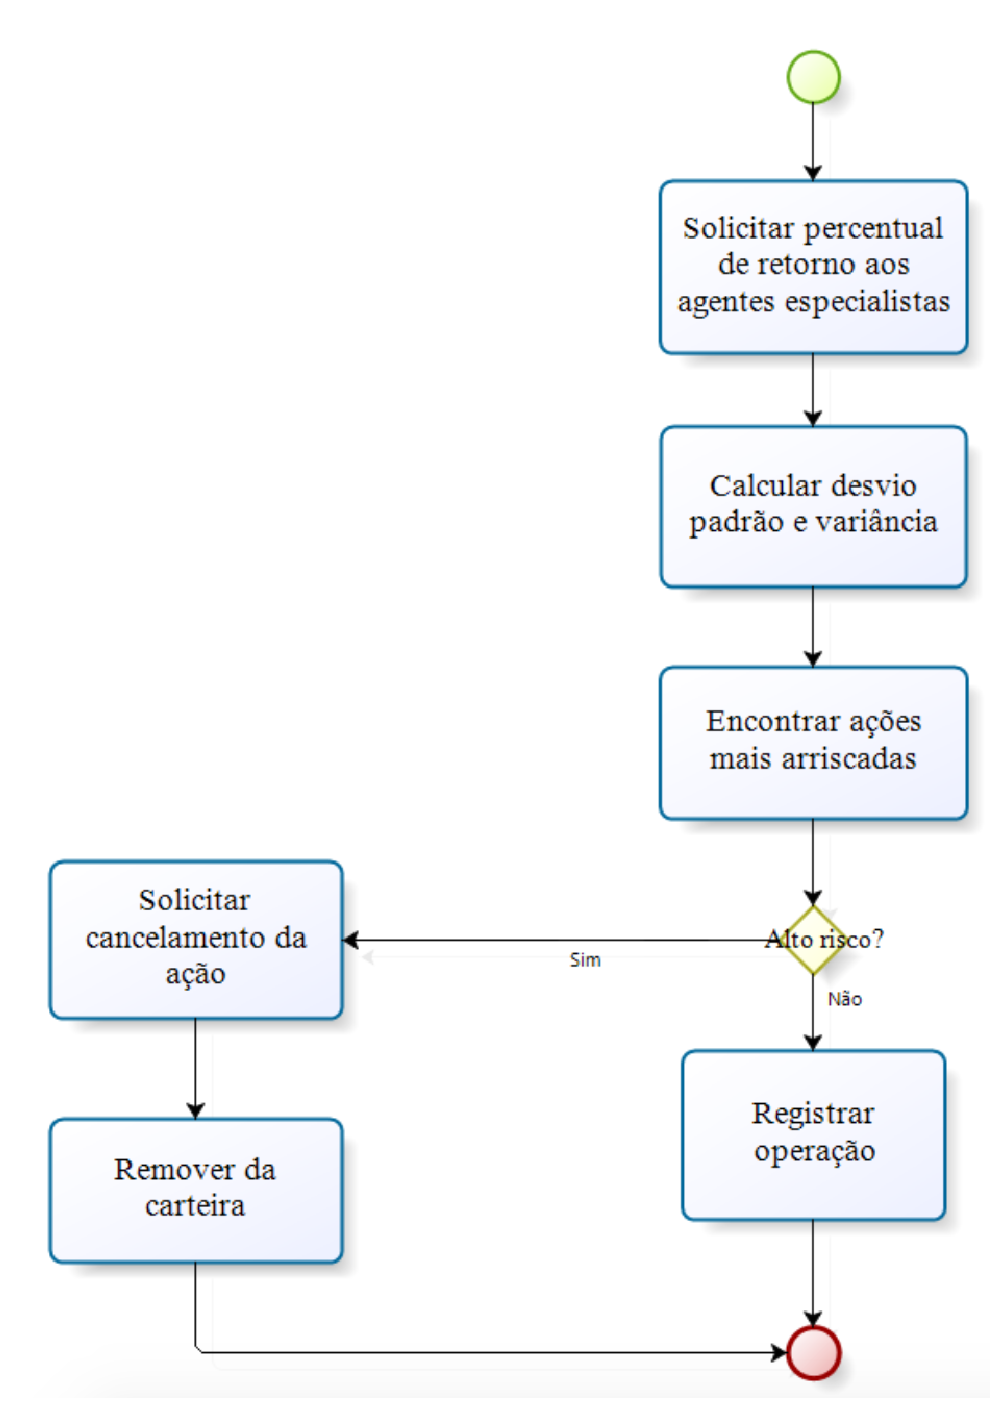
\includegraphics[width=0.7\textwidth]{figuras/f15}
\caption{Processo de monitoramento de risco}
\end{figure}
\FloatBarrier

\end{itemize}

\item[Agente especialista (expert):]
O agente especialista é o agente responsável por realizar leituras constantes do mercado de valores em busca de novas cotações das ações sob sua responsabilidade. Ele é criado pelo seu agente gestor e executa estratégias compatíveis com o perfil escolhido pelo usuário. Recebe ainda um grupo de ações, ficando responsável pelas cotações das mesmas. Durante o desenvolvimento, verificou-se a necessidade de transferir a responsabilidade de mensurar riscos para o seu agente gestor. Suas responsabilidades são:

\begin{itemize}
\item Executar estratégias financeiras:\newline

Consiste no uso das estratégias financeiras implementadas para esta ferramenta. É através de uma estratégia financeira que um agente especialista age na Bolsa de Valores de São Paulo, ela é seu mecanismo de raciocínio. As estratégias financeiras adotadas para a ferramenta desenvolvida são compostas pelos seguintes indicadores financeiros: 

\begin{enumerate}
\item Média Móvel Simples (MMS) e Médias Móveis Exponeciais (MME):\newline

Médias móveis são médias de preços que se deslocam no tempo, ou seja, para um novo valor de entrada, há a saída de um valor antigo do cálculo. Com as médias móveis é possível suavizar a movimentação do mercado e, dessa forma, identificar tendências \cite[p.68]{matsura2006}. Ao se calcular uma média móvel, é escolhida, primeiramente, qual a quantidade de valores que será utilizada no cálculo. Se utilizamos 5 valores, tem-se, então, uma média de 5 períodos, e assim por diante. Depois, define-se o tipo da média móvel. Para esta ferramenta, são as médias móveis simples e exponenciais.

A Média Móvel Simples (figura 25) é uma média com tempo de reação mais lento dentre as médias. Ela é bastante utilizada para identificar tendências de alta ou de baixa no Mercado Financeiro. Quanto maior a sua periodicidade, mais lenta ela será. Médias de alta periodicidade, normalmente, são utilizadas em estratégias de longo prazo \cite[p. 69]{matsura2006}.

\begin{figure}[h]
\centering
\label{f25}
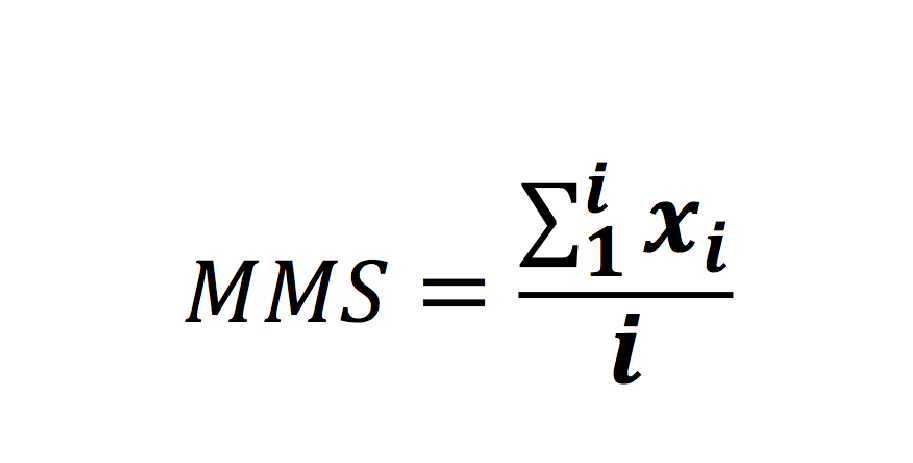
\includegraphics[width=0.5\textwidth]{figuras/f22}
\caption{Média Móvel Simples}
\end{figure}

A Média Móvel Exponencial (figura 26) é mais ágil em relação à média simples. Ela confere peso maior aos valores mais recentes, e com isso se torna uma média mais sensível às oscilações do Mercado Financeiro. Na figura 27, a variável \textbf{F} representa o valor de fechamento de uma ação, \textbf{N} representa o número de períodos da média, e \textbf{K} representa a constante calculada.

\begin{figure}[h]
\centering
\label{f26}
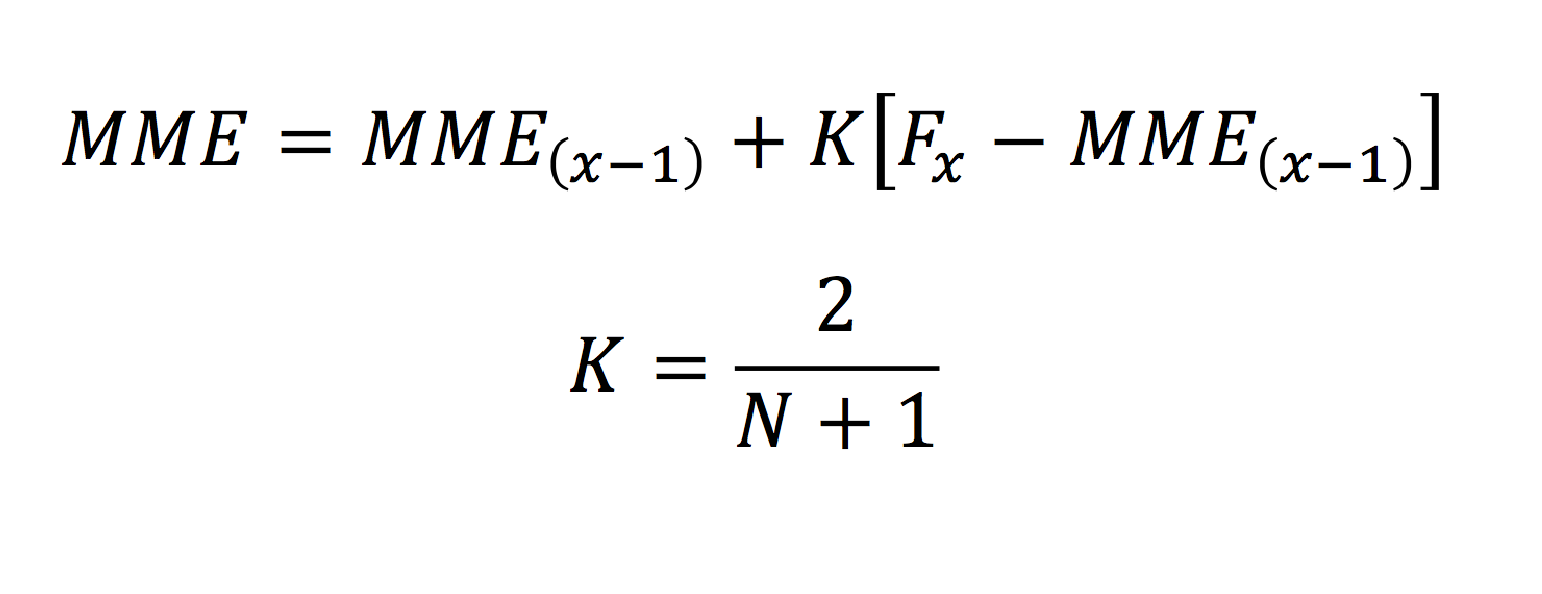
\includegraphics[width=0.5\textwidth]{figuras/f23}
\caption{Média Móvel Exponencial}
\end{figure}
\FloatBarrier

\item Darkcloud:\newline
O padrão de formação Dark cloud (figura 27) é composto por duas candlesticks, a primeira de alta, em branco, e a segunda de baixa, em vermelho. Elas são precedidas de uma tendência de alta confirmada da ação. A segunda candlestick tem valor de abertura superior ao valor de fechamento da primeira, e tem valor de fechamento superior ao valor de abertura da primeira candlestick. Este padrão de formação indica reversão da tendência de alta para baixa \cite[p.61]{matsura2006}. Tal fato será utilizado para sinalizar oportunidades de venda de ações.

\begin{figure}[H]
\centering
\label{f27}
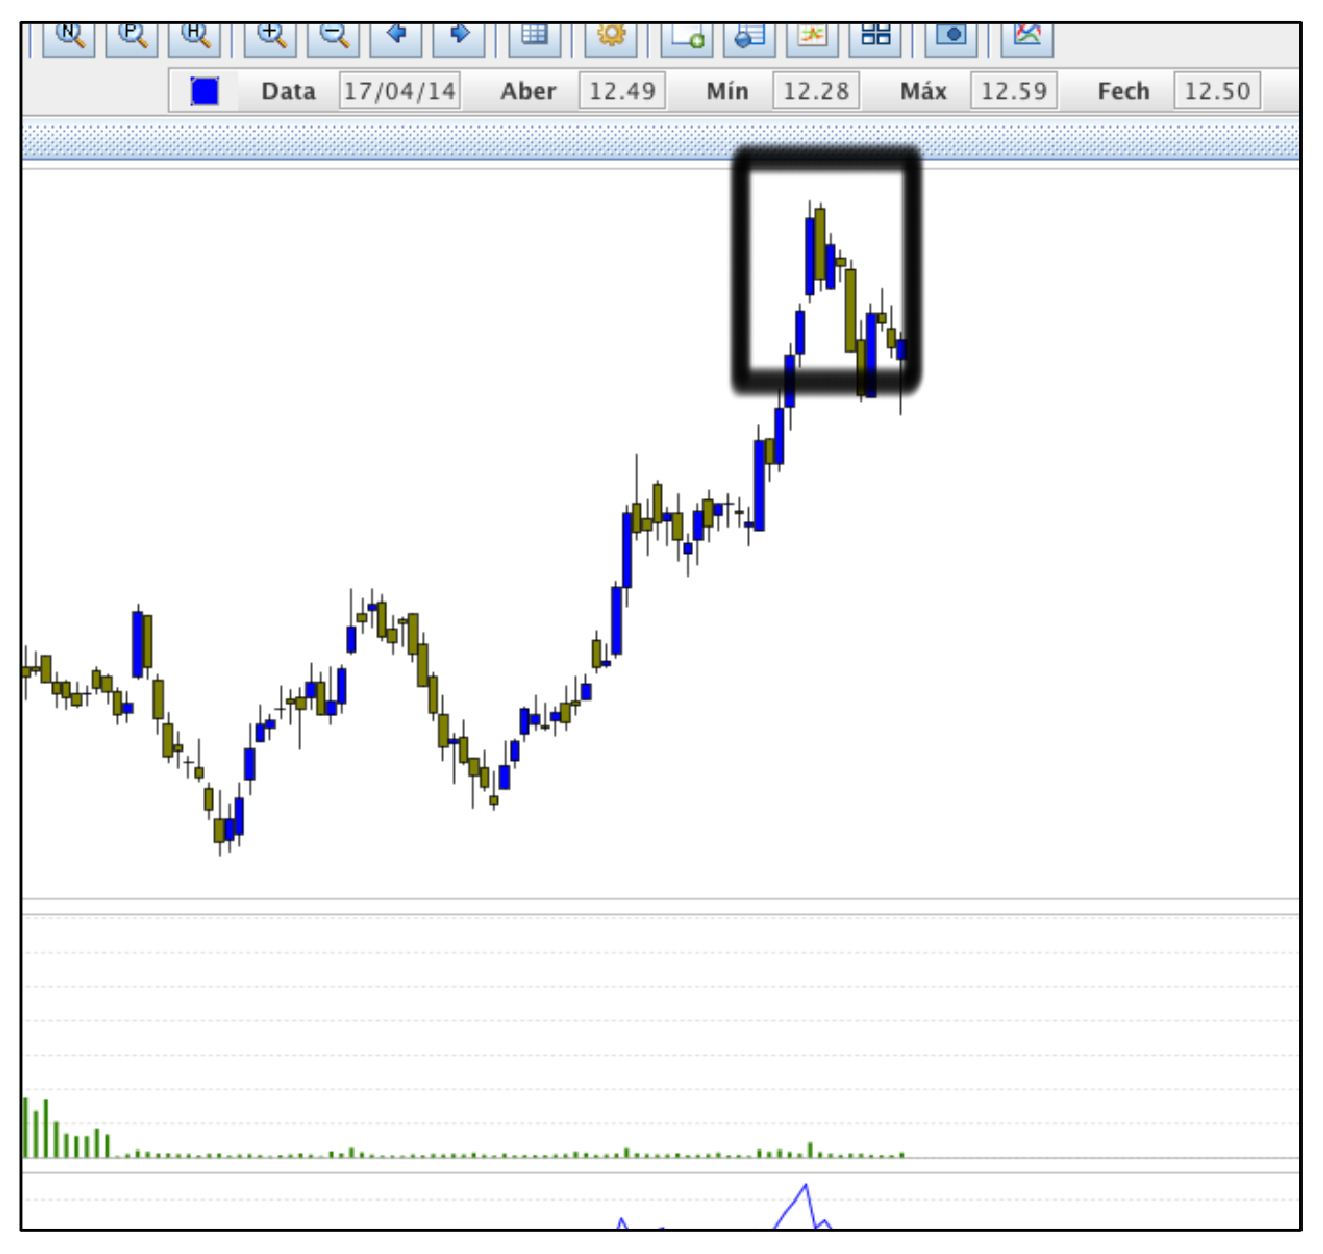
\includegraphics[width=0.9\textwidth]{figuras/f19}
\caption{Padrão DarkCloud}
\end{figure}
\FloatBarrier
\item Bearish Engulfing:\newline
O padrão de formação Bearish Engulfing (figura 28), assim como o Darkcloud, sinaliza a reversão de um tendência de alta de uma ação. No entanto, este padrão difere-se por sua segunda candlestick ter valor de fechamento inferior ao valor de abertura da primeira \cite[p. 38]{bigalow2010}.

\begin{figure}[H]
\centering
\label{f28}
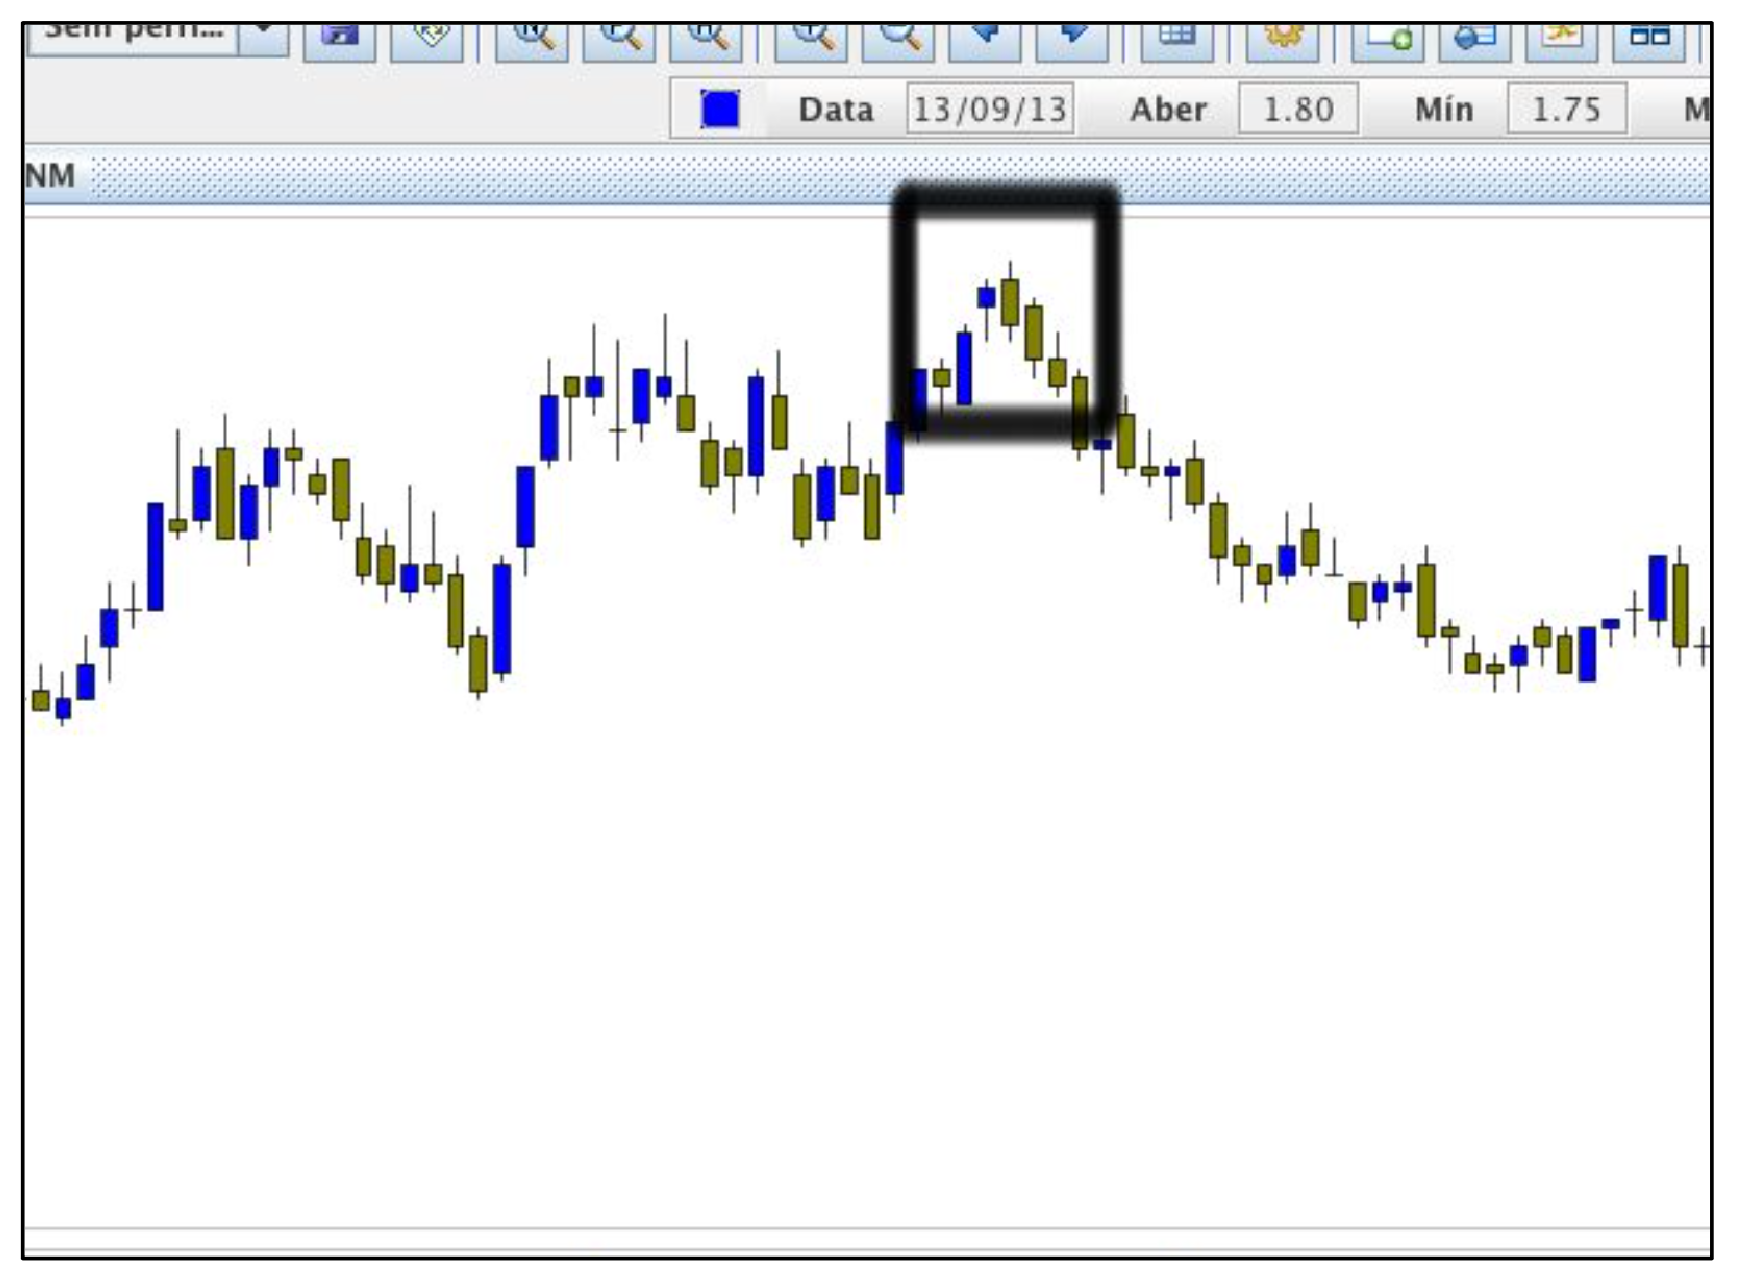
\includegraphics[width=0.9\textwidth]{figuras/f21}
\caption{Padrão Bearish Engulfing}
\end{figure}

\item Bullish Engulfing:\newline

O padrão de formação Bullish Engulfing (figura 29) é um padrão de reversão de tendência similar ao Bearish Engulfing. Este padrão é precedido de uma tendência de baixa, e sinaliza oportunidade de compra de ações. É composto por duas candlesticks, a primeira de baixa fecha de acordo com a tendência (i.e. uma candlestick de baixa). A segunda tem seu valor de abertura inferior ao valor de fechamento da primeira, e seu valor de fechamento maior do que o valor de abertura da primeira \cite[p. 36]{bigalow2010}.

\begin{figure}[H]
\centering
\label{f29}
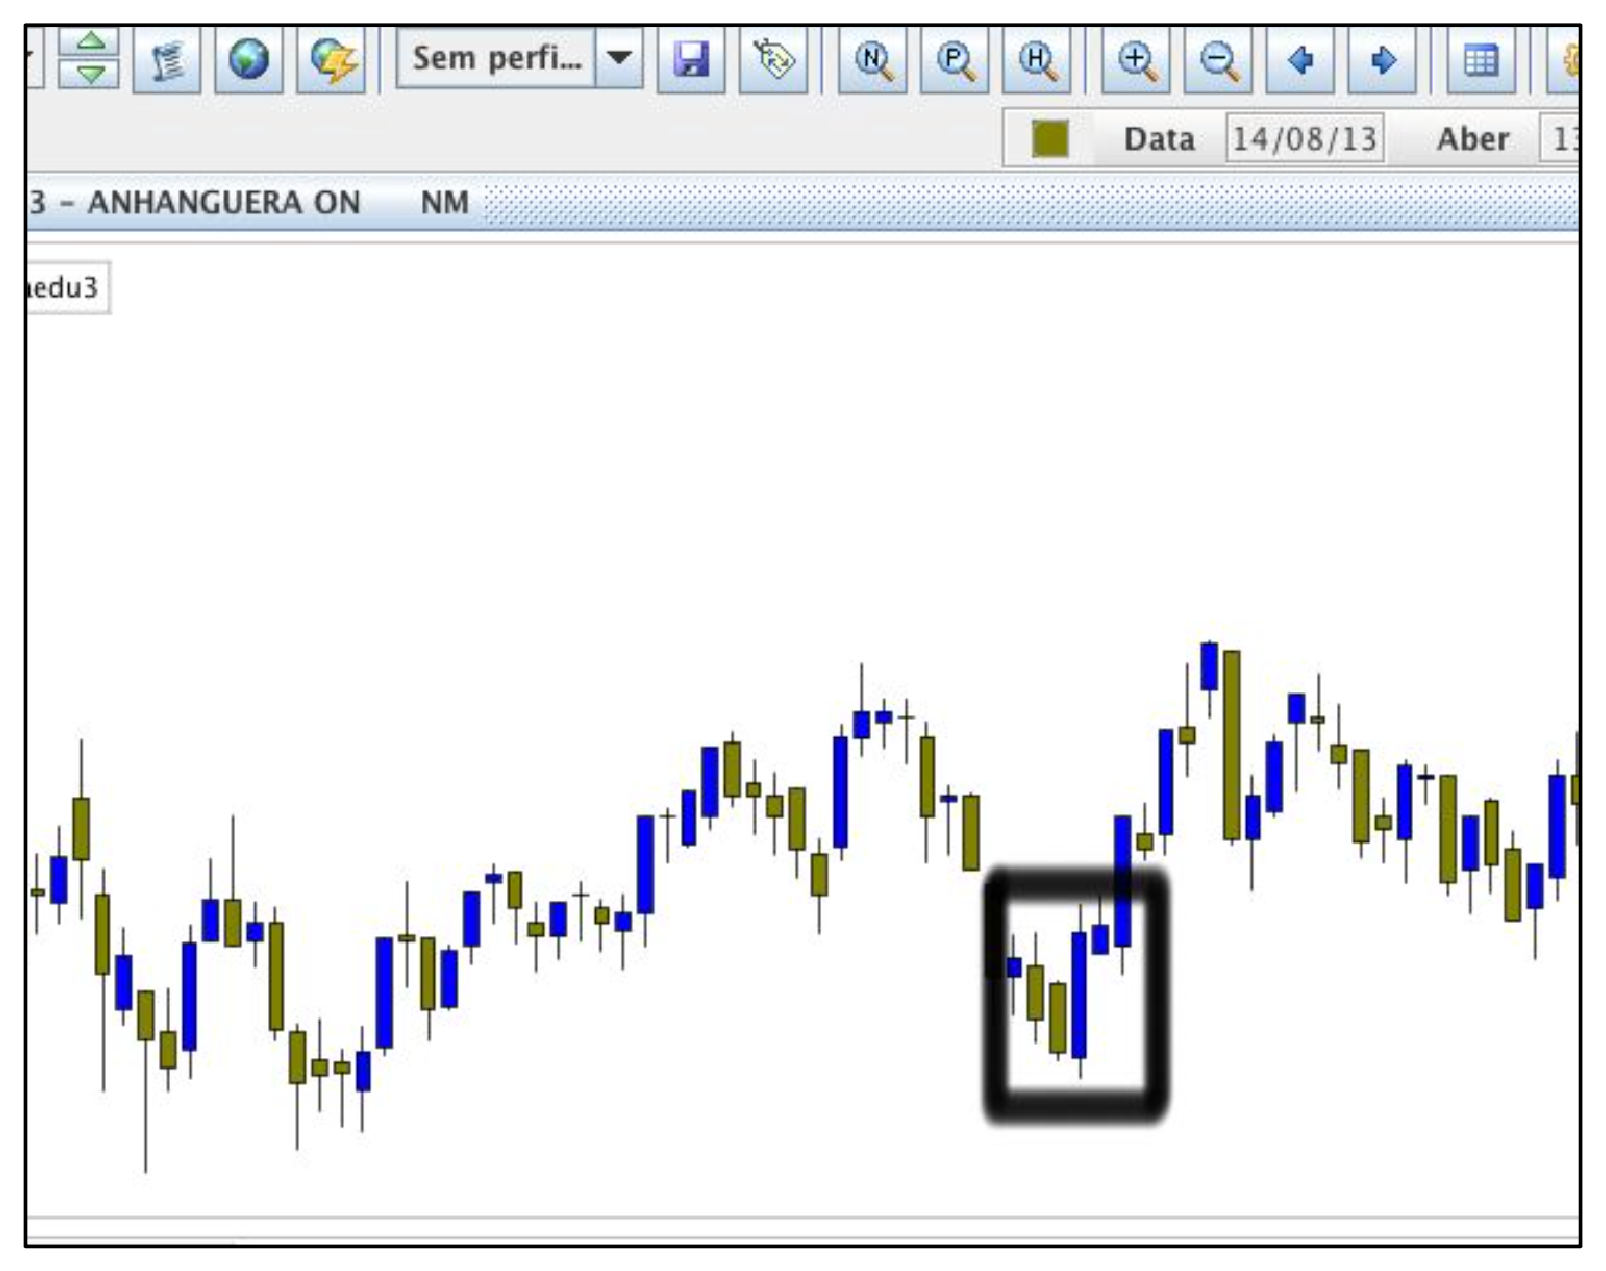
\includegraphics[width=0.9\textwidth]{figuras/f20}
\caption{Padrão Bullish Engulfing}
\end{figure}
\FloatBarrier

\end{enumerate}


Adicionalmente, foram implementadas classes que representam  estratégias financeiras que fazem uso de combinações destes indicadores, como apresentado na Tabela 9.

\begin{center}
\begin{longtable}{| p{2cm} | p{2cm} |p{3cm} |p{3cm} |}
\caption{Estratégias por perfil} \\
\hline
\textbf{Perfil} & \textbf{Estratégia 1} & \textbf{Estratégia 2}& \textbf{Estratégia 3}\\\hline
\endfirsthead
\multicolumn{2}{c}%
{\tablename\ \thetable\ -- \textit{Continuação da página anterior}} \\\hline
\textbf{Perfil} & \textbf{Estratégia 1} & \textbf{Estratégia 2} & \textbf{Estratégia 3} \\ \hline
\endhead
\hline \multicolumn{2}{c}{\textit{Continuaçao na próxima página}} \\
\endfoot
\hline
\endlastfoot
	Corajoso & MME (13/21) & Dark Clould + Bullish Engulfing. & Bearish Engulfing + Bullish Engulfing\\ \hline
	Moderado & MMS(13/21) & MME(13/21) & MME(13/21) \\\hline
	Conservador & MMS(13/21) & MMS(21/34)& MME(21/34)
\label{t09}
\end{longtable}
\end{center}


\item Solicitar autorização para realizar compra ou venda de ações:\newline
Consiste na interação com o agente gestor quando há algum sinal de compra ou venda de ações. Quando o agente especialista detecta, através de sua estratégia financeira, um sinal de compra ou venda, este solicita ao agente gestor a autorização, que por sua vez envia para o usuário na forma de sugestão quando o mesmo realizar o \textit{log in} na ferramenta.

\end{itemize}
 

\item[Agente caçador (hunter):]
O agente caçador é responsável por fazer buscas constantes de cotações de ações presentes na Bolsa de Valores e trabalhadas pela ferramenta. Suas responsabilidades são: 

\begin{itemize}
\item Baixar e atualizar o banco de dados:\newline
Consiste em realizar \textit{downloads} de cotações de ações continuamente e atualizar os dados estatísticos no banco da dados. 
\item Categorizar ações utlizando critérios estatísticos:\newline
Consiste em realizar uma categorização de ações através de valores estatísticos, tais como: (i) retorno médio diário; (ii) retorno médio 15 e 30 dias; (iii) variância média diária; e (iv) variância média 15 e 30 dias. Através destes valores, o agente caçador seleciona grupos de ações compatíveis com os perfis informados por agentes gestores no procedimento de montagem de carteira.
\item Selecionar grupo de ações de acordo com o perfil de usuário:\newline
Consiste em selecionar um grupo de ações usando como critério de seleção a variância combinada ao perfil de usuário.
\end{itemize}

\item[Agente criador (criator):]
 O agente criador é responsável por auxiliar a comunicação entre os usuários e seus respectivos grupos de agentes. Suas responsabilidades são: 

\item Monitorar a criação de novas contas:\newline

Consiste em monitorar o casdastro de usuários. Quando uma conta é criada, o agente criador captura as informações repassadas pelo usuário e instancia um agente gestor para este usuário. Em sequência, informa a esse agente gestor, através de uma mensagem com informações do usuário, tais como: nome, o valor investido e perfil escolhido.

\item Monitorar \textit{Log In} de usuários:\newline
Consiste em monitorar a autenticação de usuários na interface web. Quando um usuário autentica-se na ferramenta, o agente criador informa ao seu agente gestor para que o mesmo se comunique com seu usuário. A comunicação entre o agente gestor e seu respectivo usuário é demonstrado na figura 30, bem como o funcionamento geral da ferramenta.

\end{description}

\begin{figure}[h]
\centering
\label{f30}
\includegraphics[width=1\textwidth]{figuras/visaoGeralFerramenta}
\caption{Visão geral da ferramenta}
\end{figure}
\FloatBarrier


\section{Abordagem para Manutenção Evolutiva da Ferramenta}

A Ferramenta de Software desenvolvida foi desenhada de maneira a facilitar sua evolução. A figura 23 apresenta de maneira sucinta o uso de programação baseada em interfaces. O uso de interfaces, como orientado pelo padrão de projeto Strategy, permite a criação de novas estratégias financeiras, sejam estratégias baseadas em análise técnica ou análise fundamentalista. Este é um ponto importante para manutenções evolutivas no tocante ao contexto financeiro.

No tocante a Sistemas Multiagentes, durante o desenvolvimento da Ferramenta proposta e após seguir as práticas adotadas pelas literaturas relacionadas à implementação de agentes com o JADE, o desenvolvedor elaborou uma estrutura baseada em interfaces de maneira a reduzir o acoplamento de classes que implementam agentes comportamentais, bem como facilitar futuras manutenções. Esta estrutura contém uma interface denominada ProcedureBehaviour e uma classe concreta denominada CommunicationBehaviour, e é uma sugestão de refatoração para a Ferramenta de Software, figura 31.

\begin{figure}[h]
\centering
\label{f31}
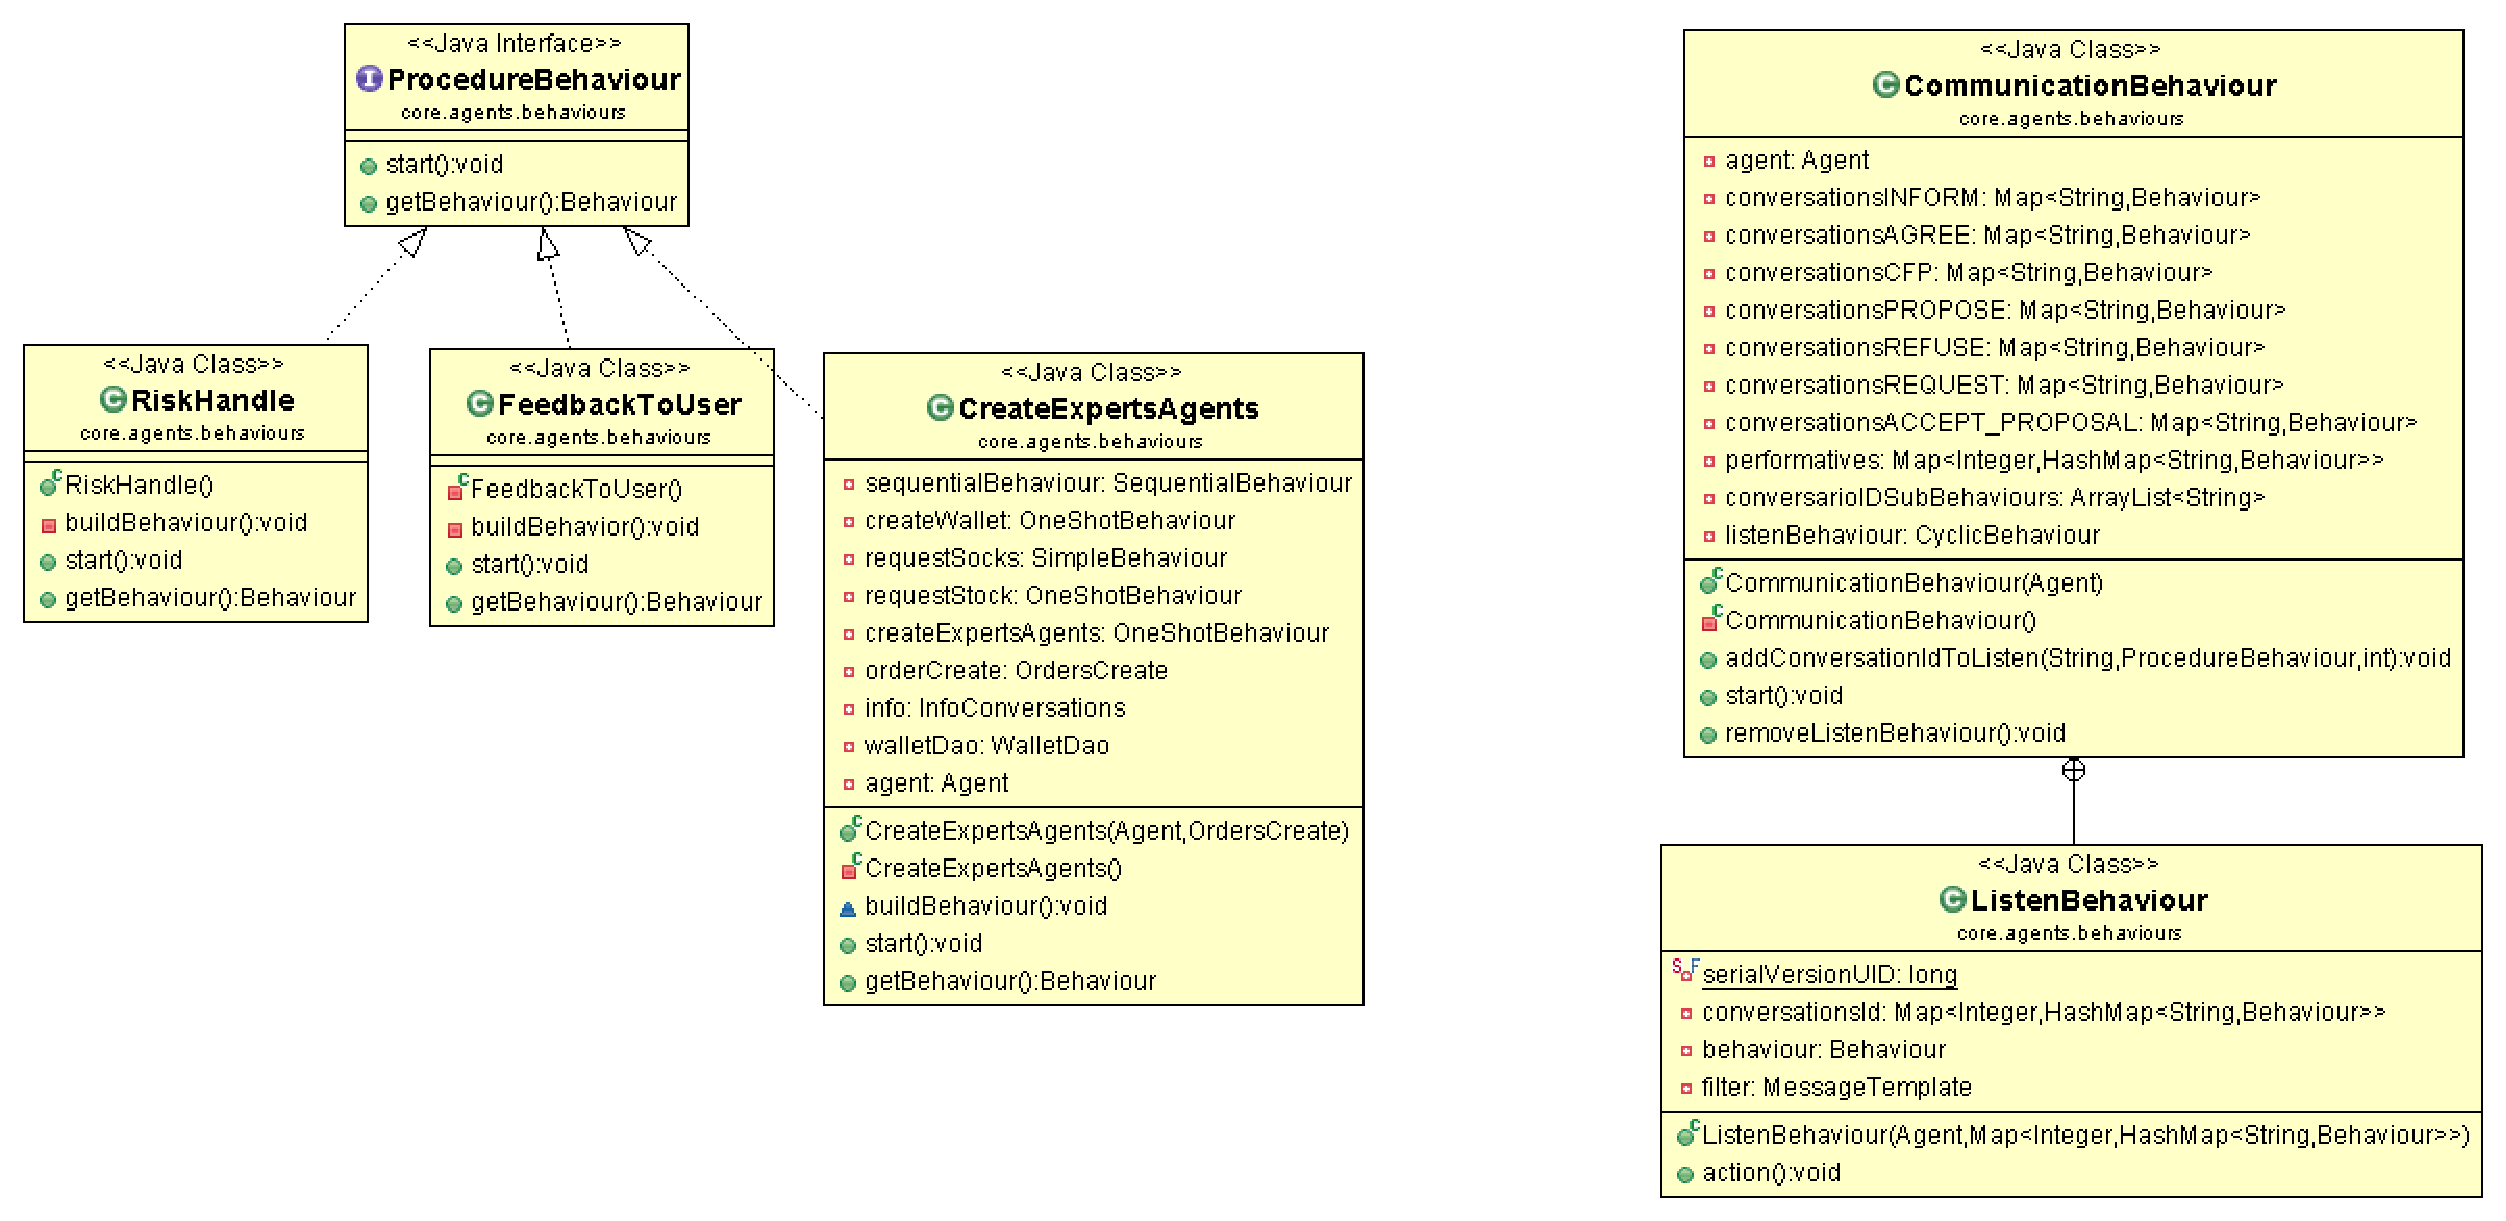
\includegraphics[width=1\textwidth]{figuras/pacoteBehaviours}
\caption{Estrutura sugerida para refatoração}
\end{figure}
\FloatBarrier

A Classe CommunicationBehaviour implementa o comportamento em comum entre os agentes comportamentais, o qual consiste em receber mensagens de outros agentes e responder estas mensagens através da execução de um comportamento. Esta classe dispõe de um mecanismo de adição de comportamentos, no qual, para que essa adição seja feita, é necessário informar a classe, os atributos ConversationID e uma classe concreta ProcedureBehaviour. Esta classe agente pode utilizar a agregação para aplicar o seu conjunto de comportamentos, assim reduzindo o acoplamento da classe e aumentando sua coesão.

\section{Resumo do Capítulo}

Elucidou-se neste capítulo o detalhamento da arquitetura desenhada para a ferramenta. Essa arquitetura orientou-se de acordo com o padrão arquitetural Model-View-Controller (MVC). Adicionalmente, foi apresentada a arquitetura da máquina de raciocínio dos agentes implementados, esta composta por quatro tipos de agentes: (i) agente gestor, responsável por administrar uma carteira de ações; (ii) agente especialista, responsável identificar sinais de compra e venda de ações através de estratégia financeira; (iii) agente caçador,  responsável por baixar cotações e persistir dados estatísticos de ações; e (iv) agente criador, responsável por auxiliar a comunicação entre os usuários e seus respectivos agentes gestores.
Adicionalmente, foi apresentada uma estrutura baseada em interfaces sugerida para facilitar a manutenção bem como a refatoração da ferramenta.  


\newpage
\chapter[RESULTADOS]{Resultados}

Nesse capítulo, serão apresentados os principais resultados obtidos usando uma abordagem híbrida quantitativa e qualitativa, conduzida com pesquisa-ação combinada a cenários de uso. A parte quantitativa está apoiada em simulações realizadas na ferramenta. Já a parte qualitativa está apoiada em feedbacks dos usuários que participaram dos testes realizados na ferrramenta. A cada iteração da pesquisa-ação, foram coletadas as respectivas impressões quanto aos testes realizados.

\section{Análise Quantitativa}
\subsection{Teste Unitários e Coberturas de Código}

Foram adotadas as ferramentas JUnit e Eclemma para a realização dos testes nos códigos referentes ao suporte, tais como: (i) os códigos que implementam a camada de persisitência da ferramenta; (ii) os códigos que implementam algoritmos estatísticos utilizados pelos agentes caçadores e gestores; (iii) os códigos que implementam as estratégias financeiras utilizadas pelos agentes especialistas; e (iv) os códigos que implementam as classes de suporte a comportamentos utilizadas pelos agentes gestores e especialista. O propósito do uso dos teste unitários foi validar os algoritmos de suporte, este essenciais para o funcionamento da ferramenta. Assim, foi estabelecida a meta de 90\% de cobertura de testes.

Quanto aos códigos que implementam os agentes comportamentais, estes não possuem, até o presente momento, uma ferramenta de validação comportamental adequada. Diante disto, foram migradas todas as rotinas utilizadas por comportamentos dos agentes, para classes que podem ser testadas através da ferramenta JUnit. A figura 32 apresenta a cobertura obtida da ferramenta em si. Vale ressaltar, que o JUnit não é a ferramenta mais adequada para o teste de classes que possuem comportamentos utilizados por agentes. Assim, a meta de cobertura de testes unitários estabelecida para este Trabalho de Conclusão de Curso se aplica somente para as classes contidas no pacote rcs.suport.

\begin{figure}[h]
\centering
\label{f22}
\includegraphics[width=0.8\textwidth]{figuras/junit2}
\caption{Cobertura de testes unitários}

\end{figure}
\FloatBarrier


\subsection{Métricas de Qualidade de Código}

Segundo Filho (\citeyear{filho2013}, p.1), medir e monitorar a qualidade do software é fundamental, independentemente da metodologia de desenvolmento adotada. Ele afirma ainda que muitos fatores que compõem um bom software podem ser percebidos no código fonte. E mesmo que se possua uma ótima suite de testes, esta não é capaz de produzir informações acerca de itens de qualidade, tais como : (i) manutenabilidade; (ii) modularidade; (iii) flexibilidade e (iv) simplicidade. Assim, não é recomendado negligenciar as métricas de código em relação a outras abordagens de monitoramento da qualidade. Diante disso, as duas características fundamentais que nortearam o desenvolvimento da ferramenta resultado deste Trabalho de Conclusão de Curso foram, a manutenabilidade e a reusabilidade. Estas consideradas importantes pelo autor por contribuirem em termos de facilidade de evolução da ferramenta. 

Assim, para verificar o grau de qualidade da ferramenta, no ponto de vista da qualidade de código, foram adotadas as seguintes métricas: (i) Complexidade Ciclomática - CC; (ii)  Coesão e Acoplamento  - SC; e (iii) Herança - DIT. Os valores de cada métrica foram obtidos com o auxílio da ferramenta Analizo. Esses valores são apresentados na tabela 10 e são classificados de acordo com os intervalos apresentados na figura 33.

\begin{figure}[h]
\centering
\label{f25}
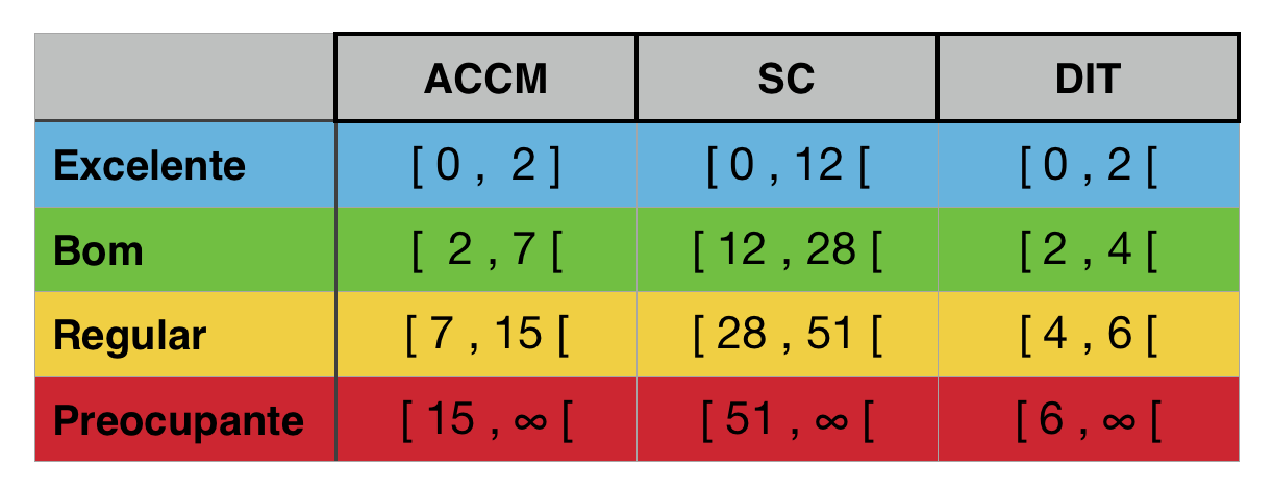
\includegraphics[width=0.9\textwidth]{figuras/metricas}
\caption{Intervalo para interpretação das métricas.\newline Fonte:\cite{filho2013}}
\end{figure}

\begin{center}
\begin{longtable}{| p{2cm} | p{2cm} |p{4cm} |}
\caption{Métricas de código fonte} \\
\hline
\textbf{Nome} & \textbf{Valor} & \textbf{Classificação} \\ \hline
\endfirsthead
\multicolumn{2}{c}%
{\tablename\ \thetable\ -- \textit{Continuação da página anterior}} \\
\hline
\textbf{Nome} & \textbf{Valor} & \textbf{Classificação} \\ \hline
\endhead
\hline \multicolumn{2}{c}{\textit{Continuaçao na próxima página}} \\
\endfoot
\hline
\endlastfoot

	CC/ACCM & 3.97 & Bom \\ \hline
	SC & 12.07 & Bom \\ \hline
	DIT & 0.36 & Excelente
	
\label{t10}
\end{longtable}
\end{center} 

Por fim, diante dos dados apresentados na tabela 10, pode-se concluir que a ferramenta desenvolvida neste Trabalho de Conclusão de Curso possui uma arquitetura que contribui com a manutenibilidade e a reusabilidade. 

\section{Análise Qualitativa}

\subsection{Pesquisa - Ação}
Segundo Rocha, pesquisa-ação pode ser considerada "independente" e "objetiva". E de acordo com Thiollent \apud{thiollent1986} {rocha2012}, caracteriza-se pesquisa-ação como:
\begin{citacao}
Um tipo de pesquisa social com base empírica, concebida e realizada em estreita associação com uma ação ou com a resolução de um problema coletivo no qual os pesquisadores e os participantes, representativos da situação e/ou do problema, estão envolvidos de forma cooperativa e participativa \apud[p. 3]{thiollent1986} {rocha2012}.
\end{citacao}

\newpage
A pesquisa-ação é um processo cíclico e contínuo, onde se planeja, implementa, descreve e avalia uma mudança para a melhoria de sua prática. Desta forma, há um aprendizado maior por parte do pesquisador durante o processo. Neste trabalho, o processo de pesquisa-ação foi utilizado para verificar o objetivo específico, sob o ponto de vista da interface com usuário, no caso: "Abstrair a complexidade de cálculos financeiros comumente utilizados na Análise Técnica. Assim, essa complexidade não é sentida pelo usuário, deixando a mesma a cargo da ferramenta.". O cenário de uso bem como os resultados obtidos são apresentados nos tópicos seguintes. Em resumo, serão apresentadas as principais etapas para condução da coleta de impressões com os potenciais usuários da ferramenta. Posteriormente, serão descritos, na ordem: os objetivos dessa coleta, o público alvo avaliado, as observações coletadas e as ações tomadas.

\subsection{Coleta de Impressões: Usuários}



A coleta de dados foi organizada de acordo com as seguintes etapas: 
\begin{itemize}
\item Planejamento:\\
Nesta etapa foram levantadas questões a serem respondidas pelos potenciais usuários de maneira a avaliar a interface gráfica da ferramenta;

\item Implementação:\\
Nesta etapa foi elaborado um questionário (figura 34 e 35) a ser respondido pelos usuários, e foi disponibilizado ainda um cenário tecnológico onde a ferramenta apresentou dados em um período histórico de cotações da BM\&FBovespa;

\begin{figure}[h]
\centering
\label{f34}
\includegraphics[width=0.7\textwidth]{figuras/questionario_1}
\caption{Questionário aplicado.}
\end{figure}

\begin{figure}[h]
\centering
\label{f34}
\includegraphics[width=0.7\textwidth]{figuras/questionario_2}
\caption{Questionário aplicado.}
\end{figure}
\FloatBarrier

\item Descrição:\\
Nesta etapa, concentra-se a descrição do cenário de uso da ferramenta. Quanto à descrição do cenário de uso, tem-se que o mesmo é apresentado a seguir:

\begin{adjustwidth}{1,5cm}{0cm}
 \textit{A Ferramenta foi apresentada aos potenciais usuários em modo de simulação no período de 1 de março de 2013 a 1 de março de 2014, a versão do JADE utilizado é a 4.3.3 de 10 de dezembro de 2014, a versão do Grails foi a 2.4.3 e a versão do java foi a 1.7.0\_79. A ferramenta foi simulada ainda em um notebook da marca Apple modelo MacBook Pro (Retina, 13-inch, Late 2013) com processador 2.6 GHz Intel Core i5, com 8 GB 1600 MHz DDR3 de Memória RAM e com o Sistema operacional OS X Yosemite versão 10.10.3.} 
\end{adjustwidth}

\item Avaliação e Ação:\\
Nesta etapa foram coletados os \textit{feedbacks} dos potenciais usuários da ferramentas em primeiro momento; no segundo momento, foram tomadas ações de ajustes da interface da ferramenta, sendo apresentada novamente aos usuários. Dentre os \textit{feedbacks} recebidos, destacou-se a sugestão de um usuário que se identificou com o perfil Corajoso, onde ele sugeriu usar outro indicador no lugar do indicador Média Móvel. As informações coletadas são expostas de maneira sucinta neste tópico e na íntegra no Apêndice E.
\end{itemize}
\begin{description}

\item[Objetivos:]
Esta coleta de dados com potenciais usuários teve como principal propósito verificar o objetivo específico: “Abstrair a complexidade de cálculos financeiros comumente utilizados na Análise Técnica. Assim, essa complexidade não é sentida pelo usuário, deixando a mesma a cargo da ferramenta”. Vale ressaltar que essa avaliação teve como foco a interface gráfica da ferramenta com os usuários, onde cada usuário recebeu um formulário com questões objetivas e um campo livre para sugestões. O comportamento dos agentes bem como os resultados das estratégias abordadas foram avaliados através de simulações.

\item[Público alvo avaliado:]

A avaliação ocorreu em maio de 2014 e participaram da avaliação seis pessoas, onde: 1 se classifica no perfil Corajoso; 1 se classifica no perfil Moderado e 4 se classificam no perfil Conservador. O teste funcional da ferramenta foi feito com uso de dados históricos no período entre 1 de março de 2014 e 3 de março de 2015. A inteface gráfica da ferramenta foi o foco dessa primeira análise.

\item[Observações coletadas:]
Quando questionados sobre as cores adotadas na ferramenta, 5 pessoas consideraram boas e 1 pessoa considerou ótima. Quando questionados sobre a facilidade de compreensão da ferramenta, 3 pessoas consideraram como bom, 1 pessoa considerou razoável, 1 pessoa considerou como ruim e 1 se absteve. Quando solicitadas observações gerais para melhoria da ferramenta, destacaram-se: (i) feedback indicando o carregamento e o processo da ferramenta; (ii) atualização da página principal automaticamente; (iii) disponibilidade de um canal de dúvidas; (iv) não adoção de estratégias baseadas em Médias Móveis; (v) utilização de javascript na interface; (vi) execução da ferramenta em duas máquinas, e (vii) disponibilidade de informações sobre estratégias e uso da ferramenta.

As sugestões apresentadas pelos usuários demandaram melhorias na interface gráfica, como esperado, e uma demanda na melhoria das estratégias adotadas. Para atender a demanda de melhorias na interface gráfica, foi necessário realizar pequenas capacitações em tecnologias front-end, tais como: javaScript e jQuery. Para atender a demanda de melhorias nas estratégias, foi necessário criar novas estratégias baseadas em outros indicadores financeiros e simular novamente a estratégia.

\item[Ações Tomadas:]

Foram feitos ajustes na interface, dentre eles: (i) a criação um canal de comunicação por onde os usuários podem enviar dúvidas, sugestões entre outros; (ii) a criação de uma página com informações importantes da ferramenta; e (iii) a inserção de um mecanismo de requisição automática na página principal. Após as melhorias, a ferramenta foi apresentada novamente aos usuários e verificou-se que as melhorias foram aceitas e novos feedbacks foram coletados.Ao final do ciclo pesquisa-ação, foram registradas algumas demandas de manutenção evolutiva da ferramenta, tais como a inserção de estratégias baseadas em outros indicadores financeiros. Neste caso, optou-se pelo uso de padrões de projeto, como o Strategy, visando facilidades orientadas à manutenção, reutilização e extensibilidade. Detalhes sobre a abordagem de manutenção evolutiva utilizada encontram-se no capítulo 5, sobre a ferramenta. 

\end{description}

\subsection{Coleta de Impressões: Simulações de Estratégias}

Esta coleta de dados foi organizada de acordo com as seguintes etapas:
\begin{itemize}
\item Planejamento:\\
Nesta etapa, foi definido um intervalo de tempo para simular as estratégias financeiras;
\item Execução:\\
Nesta etapa, foram feitas simulações utilizando os três perfis de usuários;
\item Avaliação:\\
Nesta etapa, foram feitas interpretações dos dados coletados em primeiro momento; Em segundo momento, foram feitos ajustes nas estratégias que apresentaram resultados não satisfatórios.
\end{itemize}

\begin{description}
\item[Objetivos:]
Esta coleta de impressões com potenciais usuários teve como principal propósito verificar  o objetivo específico: \textit{“Abstrair a complexidade de cálculos financeiros comumente utilizados na Análise Técnica. Assim, essa complexidade não é sentida pelo usuário, deixando a mesma a cargo da ferramenta”}. Vale ressaltar que essa avaliação teve como foco as estratégias adotadas na ferramenta.

As estratégias foram simuladas no período no período de 1 de janeiro de 2012 a 1 de março de 2015, a versão do JADE utilizada é a 4.3.3 de 10 de dezembro de 2014, a versão do Grails foi a 2.4.3 e a versão do java foi a 1.7.0\_79. A ferramenta foi simulada ainda em um notebook da marca Apple modelo MacBook Pro (Retina, 13-inch, Late 2013) com processador 2.6 GHz Intel Core i5, com 8 GB 1600 MHz DDR3 de Memória RAM e com o Sistema operacional OS X Yosemite versão 10.10.3.

\item[Observações coletadas:]

O processo de coleta de impressões foi iniciado simulando o perfil Corajoso. Ao final, as estratégias se mostraram ineficientes. No periodo simulado, as estratégias apresentaram -18,08\% de ganho, ou seja, houve uma perda de capital considerável e tal fato motivou um ajuste nas estratégias. Ao simular o perfil Moderado, as estratégias adotadas apresentaram 11,60\% de ganho. Durante a simulação percebeu-se uma oportunidade de melhoria nas estratégias adotadas. Ao simular o perfil perfil Conservador, as estratégias adotadas para este perfil apresentaram 7,8\% de ganho. Apesar do ganho, outras melhorias nas estratégias foram motivadas. As tabelas 11, 12 e 13 apresentam os resultados para os perfis Conservador, Moderado e Corajoso.

\begin{center}
\begin{longtable}{| p{2cm} | p{10cm} |p{2cm} |}
\caption{Estratégias Perfil Conservador e Resultados} \\
\hline
\textbf{Agente} & \textbf{Estratégia} & \textbf{Percentual de Ganho} \\ \hline
\endfirsthead
\multicolumn{2}{c}%
{\tablename\ \thetable\ -- \textit{Continuação da página anterior}} \\
\hline
\textbf{Agente} & \textbf{Estratégia} & \textbf{Percentual de Ganho} \\ \hline
\endhead
\hline \multicolumn{2}{c}{\textit{Continuaçao na próxima página}} \\
\endfoot
\hline
\endlastfoot

	A1 & Média Móvel Simples 13/21 & -29,06\% \\ \hline
	A2 & Media Móvel Simples 21/34 & -31,74\% \\ \hline
	A3 & Media Móvel Exponencial 21/34 & 34,96\% \\ \hline
	A4 & Media Móvel Simples  13/21 & 4,93\% \\ \hline
	A5 & Media Móvel Simples 21/34. & -60,41\% \\ \hline
	A6 & Media Móvel Exponencial 21/34. & 8,26\% \\ \hline
	A7 & Media Móvel Simples  13/21. & 59,91\% \\ \hline
	{} & \textbf{TOTAL GERAL} & \textbf{7,8\%} 
	
\label{t09}
\end{longtable}
\end{center} 


\begin{center}
\begin{longtable}{| p{2cm} | p{10cm} |p{2cm} |}
\caption{Estratégias Perfil Moderado e Resultados} \\
\hline
\textbf{Agente} & \textbf{Estratégia} & \textbf{Percentual de Ganho} \\ \hline
\endfirsthead
\multicolumn{2}{c}%
{\tablename\ \thetable\ -- \textit{Continuação da página anterior}} \\
\hline
\textbf{Agente} & \textbf{stratégia} & \textbf{Percentual de Ganho} \\ \hline
\endhead
\hline \multicolumn{2}{c}{\textit{Continuaçao na próxima página}} \\
\endfoot
\hline
\endlastfoot

	A1 & Media Móvel Exponencial 13/21 & 9,7\% \\ \hline
	A2 & Media Móvel Simples 13/21 & -24,36\% \\ \hline
	A3 & Media Móvel Exponencial 13/21 &41,89\% \\ \hline
	{} & \textbf{TOTAL GERAL} & \textbf{11,60\%} 
	

\label{t10}
\end{longtable}
\end{center} 

\begin{center}
\begin{longtable}{| p{2cm} | p{10cm} |p{2cm} |}
\caption{Estratégias Perfil Corajoso e Resultados} \\
\hline
\textbf{Agente} & \textbf{Estratégia} & \textbf{Percentual de Ganho} \\ \hline
\endfirsthead
\multicolumn{2}{c}%
{\tablename\ \thetable\ -- \textit{Continuação da página anterior}} \\
\hline
\textbf{Agente} & \textbf{Estratégia} & \textbf{Percentual de Ganho} \\ \hline
\endhead
\hline \multicolumn{2}{c}{\textit{Continuaçao na próxima página}} \\
\endfoot
\hline
\endlastfoot

	A1 & Bearish - Bullish & -34,71\% \\ \hline
	A2 & Dark Cloud - Bullish Engulf & -6,45\% \\ \hline
	{} & \textbf{TOTAL GERAL} & -\textbf{18,08\%} 
	
\label{t10}
\end{longtable}
\end{center} 

\item[Ações tomadas]

As estratégias financeiras do perfil Corajoso, associadas aos agentes especialistas foram substituídas por estratégias baseadas em Médias Moveis Exponenciais com uso de \textit{Stop Loss}. Para esta versão da Ferramenta de Software, não serão utilizadas as estratégias baseadas em padrões de Candlestick. Verificou-se, nesse caso, que para desenvolver um código capaz de identificar variações de um padrão de Candlestick, bem como validar os sinais, se falsos ou não, seria mais adequado usar uma abordagem de inteligência artificial orientada a mecanimos de aprendizagem. Tal mecanismo não é escopo deste trabalho, entretanto, trata-se de uma sugestão de melhoria para a ferramenta. Essa melhoria poderá usufruir da abordagem evolutiva adotada no desenvolvimento dessa ferramenta, ampliando ainda mais a capacidade de atuação dos agentes.


\begin{center}
\begin{longtable}{| p{2cm} | p{10cm} |p{2cm} |}
\caption{Estratégias Perfil Corajoso e Resultados} \\
\hline
\textbf{Agente} & \textbf{Estratégia} & \textbf{Percentual de Ganho} \\ \hline
\endfirsthead
\multicolumn{2}{c}%
{\tablename\ \thetable\ -- \textit{Continuação da página anterior}} \\
\hline
\textbf{Agente} & \textbf{Estratégia} & \textbf{Percentual de Ganho} \\ \hline
\endhead
\hline \multicolumn{2}{c}{\textit{Continuaçao na próxima página}} \\
\endfoot
\hline
\endlastfoot

	A1 & Media Móvel Exponencial 13/21 & 33,00\% \\ \hline
	A2 & Média Móvel Exponencial 13/21 & 72,47\% \\ \hline
	{} & \textbf{TOTAL GERAL} & \textbf{60,27\%} 
	
\label{t12}
\end{longtable}
\end{center} 

A tabela 14 apresenta os novos resultados da simulação do perfil Corajoso no mesmo período da simulação anterior. O valor do \textit{Stop Loss} foi ajustado empiricamente, e percebeu-se que 5\% é o valor ideal. Este valor de \textit{Stop Loss} foi adotado para os três perfis existentes na Ferramenta. As tabelas 15 e 16 apresentam os resultados da simulação dos perfis Conservador e Moderado com suas respectivas estratégias ajustadas. 

\begin{center}
\begin{longtable}{| p{2cm} | p{10cm} |p{2cm} |}
\caption{Estratégias Perfil Moderado e Resultados} \\
\hline
\textbf{Agente} & \textbf{Estratégia} & \textbf{Percentual de Ganho} \\ \hline
\endfirsthead
\multicolumn{2}{c}%
{\tablename\ \thetable\ -- \textit{Continuação da página anterior}} \\
\hline
\textbf{Agente} & \textbf{Estratégia} & \textbf{Percentual de Ganho} \\ \hline
\endhead
\hline \multicolumn{2}{c}{\textit{Continuaçao na próxima página}} \\
\endfoot
\hline
\endlastfoot

	A1 & Media Móvel Exponencial 13/21 & 13,80\% \\ \hline
	A2 & Media Móvel Simples 13/21 & -3,85\% \\ \hline
	A3 & Media Móvel Exponencial 13/21 & 82,45\% \\ \hline
	{} & \textbf{TOTAL GERAL} & \textbf{34,77\%} 
	
\label{t12}
\end{longtable}
\end{center} 


\begin{center}
\begin{longtable}{| p{2cm} | p{10cm} |p{2cm} |}
\caption{Estratégias Perfil Conservador e Resultados} \\
\hline
\textbf{Agente} & \textbf{Estratégia} & \textbf{Percentual de Ganho} \\ \hline
\endfirsthead
\multicolumn{2}{c}%
{\tablename\ \thetable\ -- \textit{Continuação da página anterior}} \\
\hline
\textbf{Agente} & \textbf{stratégia} & \textbf{Percentual de Ganho} \\ \hline
\endhead
\hline \multicolumn{2}{c}{\textit{Continuaçao na próxima página}} \\
\endfoot
\hline
\endlastfoot

	A1 & Média Móvel Simples 13/21 & -4,28\% \\ \hline
	A2 & Media Móvel Simples 21/34 & -8,75\% \\ \hline
	A3 & Media Móvel Exponencial 21/34 & 64,81\% \\ \hline
	A4 & Media Móvel Simples  13/21 & 50,33\% \\ \hline
	A5 & Media Móvel Simples 21/34. & 8,17\% \\ \hline
	A6 & Media Móvel Exponencial 21/34. & 25,91\% \\ \hline
	A7 & Media Móvel Simples  13/21. & 116,76\% \\ \hline
	{} & \textbf{TOTAL GERAL} & \textbf{38,58\%} 
	
\label{t11}
\end{longtable}
\end{center} 
\end{description}

\section{Resumo do capítulo}

Este capítulo elucidou as análises dos resultados obtidos com os testes realizados na ferramenta, sejam eles: (i) baseados na satisfação dos usuários ao utilizar a ferramenta, coleta qualitativa de dados, ou (ii) baseados em simulações, coleta quantitativa de dados. Quanto a análise quantitativa, foi estabelecida uma meta de cobertura de teste unitário em 90\%. Vale ressaltar que essa meta se aplicou somente às classes contidas no pacote \textit{suport}. 

Quanto à análise qualitativa, utilizou-se uma abordagem iterativa-evolutiva baseada em pesquisa-ação combinada a cenários de uso, cujo objetivo foi verificar a conformidade da ferramenta com os objtivos deste Trabalho de Conclusão de Curso.


\newpage
\chapter[CONSIDERAÇÕES FINAIS]{Considerações Finais}

Esse capítulo procura resgatar as principais contribuições oriundas desse Trabalho de Conclusão de Curso. Adicionalmente, são apresentados possíveis pontos de extensibilidade da ferramenta, os quais poderão acordar evoluções e trabalhos futuros.

\section{Principais Contribuições}

A Ferramenta de Software desenvolvida neste TCC é capaz de auxiliar cidadãos brasileiros a realizarem investimentos em bolsa de valores. Sua primeira versão faz uso de estratégias comumente referenciadas por investidores, Medias Móveis.  Entretanto, sua arquitetura foi desenhada de modo a suportar a adição de novas estratégias sem a necessidade de fazer alterações nos códigos fontes dos agentes comportamentais. Isto contribui para a manutenção evolutiva da ferramenta.

Ao usuário, não é requerido um prévio conhecimento relacionado ao contexto financeiro, a Ferramenta é capaz de abstrair a complexidade de cálculos financeiro, deixando-os a cargo dos agentes. A ferramenta, por ser Web, foi estruturada de acordo com o padrão arquitetural MVC, com a aplicação adicional de padrões de projeto. Em particular, o padrão Strategy destaca-se dentre os padrões de projeto adotados, uma vez que confere à ferramenta facilidades em termos de manutenção, refatoração, extensibilidade, e reusabilidade de código fonte.

Ressalta-se que os objetivos geral e específicos desse trabalho foram alcançados, de acordo com a análise dos resultados obtidos. Portanto, construiu-se, em atendimento ao objetivo geral, uma ferramenta de estratégia financeira apoiada por Sistemas Multiagentes Comportamentais, cuja máquina de raciocínio foi descrita em detalhes no capítulo 5 desse documento. Procurou-se, em atendimento ao primeiro objetivo específico, trabalhar estratégias visando abstrair a complexidade dos cálculos financeiros comumente utilizados na análise técnica, deixando essa complexidade aos agentes e não aos usuários finais da ferramenta. Por fim, em atendimento ao segundo e último objetivo específico, explorou-se o Paradigma de Sistemas Multiagentes Comportamentais no contexto financeiro, usando provas de conceito pontuais e pesquisa-ação combinada a cenários de uso, conforme apresentado em detalhes no capítulo 6 desse documento.


\section{Sugestões de Trabalhos Futuros}

Lembrando que a arquitetura adotada no desenvolvimento da ferramenta colabora com a manutenção evolutiva da mesma, poderão ser adicionados agentes capazes de atuar em outros contextos comumente encontrados na BM\&FBovespa, tais como: (i) Mercado de Opções; (i) Mercado de Mercadorias e Contratos Futuros; (iii) Renda Fixa, dentre outros. Adicionalmente, poderão ser incorporados agentes capazes de atuar em outras bolsas de valores em âmbito mundial, expandindo a capacidade cognitiva dos agentes com novas estratégias, novos indicadores financeiros e novas propostas de implementação (ex. implementação orientada ao Paradigma de Sistemas Multiagentes Intencionais, apoiado no Modelo BDI (\textit{Belief-Desire-Intention})).

Outro ponto de extensibilidade da ferramenta desenvolvida é a criação de uma interface \textit{mobile} com o usuário, através do desenvolvimento de aplicativos para Smartphones e Tablets. Estes, podem ser desenvolvidos para iOS, Android ou Windows Phone. Lembrando que a interface gráfica da ferramenta desenvolvida, em sua versão atual, pode ser visualizada, via browser, em diferentes dispositivos móveis. Isso é possível, pois a mesma foi construída com base no framework Grails. Esse framework já confere, às aplicações desenvolvidas com base em sua arquitetura padrão, responsividade em diferentes dispositivos móveis. Entretanto, seria interessante desenvolver a ferramenta como uma aplicação nativa, específica para dispositivos móveis.

